% REMEMBER: You must not plagiarise anything in your report. Be extremely careful.

\documentclass{l4proj}

    
%
% put any additional packages here
%
\usepackage{pdfpages}


\begin{document}

%==============================================================================
%% METADATA
\title{Level 4 Project - Virtual Turing Tumble}
\author{Luke Gall, 2298070g}
\date{March 1, 2021}

\maketitle

%==============================================================================
%% ABSTRACT
\begin{abstract}
    Turing Tumble is a Turing complete marble based game used to teach children and adults the power of small logical components and how they can be combined to create interesting computational results. Existing Turing Tumble simulators were found to be impressive but lacking the main external motivator of puzzles. We have built an accurate Turing Tumble simulator accessible on the web with puzzle playing and creation built in. Our evaluation shows that the program simulates a Turing Tumble correctly, is easy to use, and that puzzles can be successfully created and played. Future work would focus on adding features to match the functionality of other Turing Tumble simulators while more evaluation could be carried out on the learning opportunities present within the simulator.
\end{abstract}

%==============================================================================

% EDUCATION REUSE CONSENT FORM
% If you consent to your project being shown to future students for educational purposes
% then insert your name and the date below to  sign the education use form that appears in the front of the document. 
% You must explicitly give consent if you wish to do so.
% If you sign, your project may be included in the Hall of Fame if it scores particularly highly.
%
% Please note that you are under no obligation to sign 
% this declaration, but doing so would help future students.
%
\def\consentname {Luke Gall} % your full name
\def\consentdate {12 February 2021} % the date you agree
%
\educationalconsent


%==============================================================================
\tableofcontents

%==============================================================================
%% Notes on formatting
%==============================================================================
% The first page, abstract and table of contents are numbered using Roman numerals and are not
% included in the page count. 
%
% From now on pages are numbered
% using Arabic numerals. Therefore, immediately after the first call to \chapter we need the call
% \pagenumbering{arabic} and this should be called once only in the document. 
%
% Do not alter the bibliography style.
%
% The first Chapter should then be on page 1. You are allowed 40 pages for a 40 credit project and 30 pages for a 
% 20 credit report. This includes everything numbered in Arabic numerals (excluding front matter) up
% to but excluding the appendices and bibliography.
%
% You must not alter text size (it is currently 10pt) or alter margins or spacing.
%
%
%==================================================================================================================================
%
% IMPORTANT
% The chapter headings here are **suggestions**. You don't have to follow this model if
% it doesn't fit your project. Every project should have an introduction and conclusion,
% however. 
%
%==================================================================================================================================
\chapter{Introduction}

% reset page numbering. Don't remove this!
\pagenumbering{arabic}

\section{Motivation}
Turing Tumble is a marble based game where users build marble-powered mechanical computers to solve logical puzzles. The vertical board consists of various slots where different logical components are placed to direct red or blue marbles to the bottom, releasing the next coloured marble and storing the output pattern. Users can place a variety of these components to solve different puzzles with an aim to produce an expected marble pattern e.g. red,blue,red etc. The outputs can also capture different computational results including addition, storing state, and counting in binary. The game uses puzzles to provide an fun and captivating environment for users to play the game while learning how small, simple components can be combined to produce powerful results. 

The game, primarily focused on being a fun educational game for children, is also interesting enough to warrant the attention of adults and students. It is designed to be Turing complete, allowing users to build mechanical computers with the same computational expressiveness as a modern day computer. With this computational expressiveness contained within simple marbles, mechanical pieces, and a vertical board the game can be of interest to students wanting to explore a fun and unique way to compose computationally powerful configurations.  

A simulator of Turing Tumble can help open it up to a wider range of players that may initially be put off by the large and fairly expensive physical version. This project focuses on the creation of program that includes an accurate Turing Tumble simulator that captures the functionality of the physical board. The main aim was creating an easy to use tool for users unfamiliar with the physical game rather than adding new complex features. This allows new users to learn and play the game using the simulator while avoiding unnecessary complexity. 


\section{Goals}
\textbf{Simulate a Turing Tumble board} The main goal of the program is to provide an accurate Turing Tumble simulation. This includes correctly simulating all mechanical computer configurations that are possible within the physical version. This is required to allow users to use this program as a replacement for the physical version, without losing any accuracy or computational power. It is also important that the simulator can model a marble going down the board via a path of components while also recording the output of the mechanical computer. This will allow users to learn how a combination of small logical pieces can lead to complex results. It was decided that the board simulated in the program should follow the exact size and specifications of the physical version to be a faithful simulation while avoiding unnecessary complexity for new users to the game.

\textbf{Allow users to build their own Turing Tumble configuration} Users must be able to select and place the 6 logical components onto the various slots of a Turing Tumble board. This will allow users to create and then simulate different mechanical computer configurations. It was decided that the users should be able to place components using an on screen board to provide an easy and efficient way to create new configurations. While a text file could be used to create the different configurations, this was seen as time consuming for the user and would lead to extra complexity required to validated this input. 

\textbf{Increase learning via puzzles} Users should be able to view and play puzzles from a selection included with the official Turing Tumble game guide. The game, whilst interesting in its own right as a method of building complex configurations using simple components, can be made more of a learning opportunity for new users, by providing a set of challenging puzzles. The user should have a clear set of puzzles they can work through with different difficulty levels to keep motivation high and the challenge steady to improve the users learning experience. The puzzles can be used to teach how a Turing Tumble works as well as improve logical problem solving skills.    

\textbf{Should be easy to use and understand} The target audience of this program is Computer Science students interested in the game and school pupils that could use this program as a replacement for the physical version. This means that the program should be easy to use and understand for users unfamiliar with Turing Tumble. It is important that users can focus on how the board works and what they can learn from it rather than getting confused or disinterested because the program is hard to understand or follow. 

\textbf{Puzzle environment} To increase the likelihood that users are encouraged to use the site more than once it should be possible for users to create their own puzzles and upload them to the site. By allowing users to create their own puzzles they will learn more about creating logical challenges while also encouraging other users to play these puzzles. This environment can ensure that the user has multiple reasons to continue using the site after completing the original set of puzzles. This is important as it would encourage more time spent with the game, increasing the likelihood of users learning with the simulator. 

%==================================================================================================================================
\chapter{Background}
\section{Turing Tumble}
\label{section:background}
Turing Tumble is a marble based game designed to teach children the power of small simple components and how they can be connected together to produce mechanical computers. Fig. \ref{fig:ttboard} shows a photograph of Turing Tumble.

\subsection{Board}
Two marble dispensers are located in the top two corners of the board, one for blue and another for red marbles, each dispenser can have multiple marbles of that colour. Each marble represents 'electricity' in the computer metaphor in the game. A marble travels down the board interacting with various components that change the direction the marble will travel. At the bottom of the board it will land on a blue or red flipper which will release another marble of that colour. The marble is also stored and displayed at the bottom. The main objective of the game is to place a combination of components to create a mechanical computer that will output a certain marble pattern.



\subsection{Pieces}
\label{section:background-pieces}
There are six component types (henceforth "pieces") that represent different computer components as shown in fig. \ref{fig:physicalPieces}. Each piece is an instance of one of the component types and there are 61 pieces that can be placed. The board is filled with a criss cross pattern of Pins and Component Slots, all six types of pieces fit in \emph{Component Slots}, while only the \emph{Gear} piece fits in \emph{Pins}. Each piece has its own logic that will change the direction of a marble going down the board. The 6 pieces are described below.

\textbf{Ramp}
The Ramp (shown in fig. \ref{fig:phyRamp}) is the simplest piece and acts as a 'wire' in the computer metaphor that persists throughout the game. The Ramp sends a marble either right or left depending on the direction the curved end is facing. As the marbles aren't allowed to drop freely until they reach the end, the ramp is the most common way to direct the marbles to the desired location.

\textbf{Crossover}
The Crossover (shown in fig. \ref{fig:phyCrossover}) is a non reversible piece that continues the direction a marble is travelling into the piece and allows the marbles to enter from either side.This piece is metaphorically equivalent to wires crossing over in chips, it allows paths created using ramps and other pieces to cross over each other.

\textbf{Bit}
The Bit piece (shown in fig. \ref{fig:phyBit}) acts as a metaphorical switch that will change the direction the next marble will travel based on if it is 'on' (pointing to the right) or 'off' (pointing to the left). It sends marbles in the opposite direction it is facing. When a marble passes through a Bit it changes the direction of the piece. These pieces can be used to represent registers that store binary represented values.

\textbf{Interceptor}
The Interceptor piece (shown in fig. \ref{fig:phyInterceptor}) catches a marble and stops the execution of Turing Tumble as the marble will no longer be able to reach the end of the board and release another marble. This piece is similar to a shutoff switch inside a regular computer. 

\textbf{Gear}
Gears are the only pieces that can be placed on Pins on the board and act as connections between a number of Gear Bits. They turn either 90° left or right. 

\textbf{Gear Bit}
This piece is a like a Bit in that it stores state by pointing left or right and will send a marble in the opposite direction it is facing and then change direction. A Gear Bit not connected to a Gear will act and behave exactly like a normal Bit piece. When a Gear Bit changes direction it will also turn any connecting Gears which in turn will change the direction of any other Gear Bits and so on. The combination of this piece and the Gear is claimed to make the game 'Turing Complete'. One rule of Turing Tumble, is that all Gear Bits face the same direction to ensure that one Gear Bit turing doesn't make another Gear Bit face the wrong direction.

% Using a combination of Gear and Gear Bits it is possible to make new logical components like latches, fixed position switches, set switches, and flip flops.

\subsection{Puzzles}
\label{section:puzzle-background}
Puzzles are the main way to play Turing Tumble. The objective of a puzzle is to create a computer configuration, using a set of available pieces, that will output a desired marble pattern. The user can only trigger a marble once, meaning the output is produced by the board itself, not the user triggering multiple marbles. An example of a puzzle can be seen in fig. \ref{fig:puzzleExample}.  

The puzzle contains different attributes to describe the constraints and objectives.
\begin{itemize}
    \item Title - The name given to the puzzle.
    \item Description (Objective) - The description of a puzzle contains a one or two lines detailing the puzzles objective.
    \item Difficulty Rating - The puzzle difficulty using a 5 star scale.
    \item Starting Setup - The starting set up displays a board with the starting pieces which cannot be replaced by the user. It also includes the number of coloured marbles in each dispenser. These pieces constrain the puzzle and the way the user must meet the objective.
    \item Available Parts - The challenge of Turing Tumble puzzles come with the restriction of pieces available to match the expected output of the puzzle. This restriction ensures users follow a set configuration to meet the expected output.
    \item Required output - This displays the marble pattern that the board should output to complete the puzzle.
\end{itemize}

Details about Turing Tumble were adapted form their website \citep{turing_tumble_site}.

\begin{figure}
    \centering
    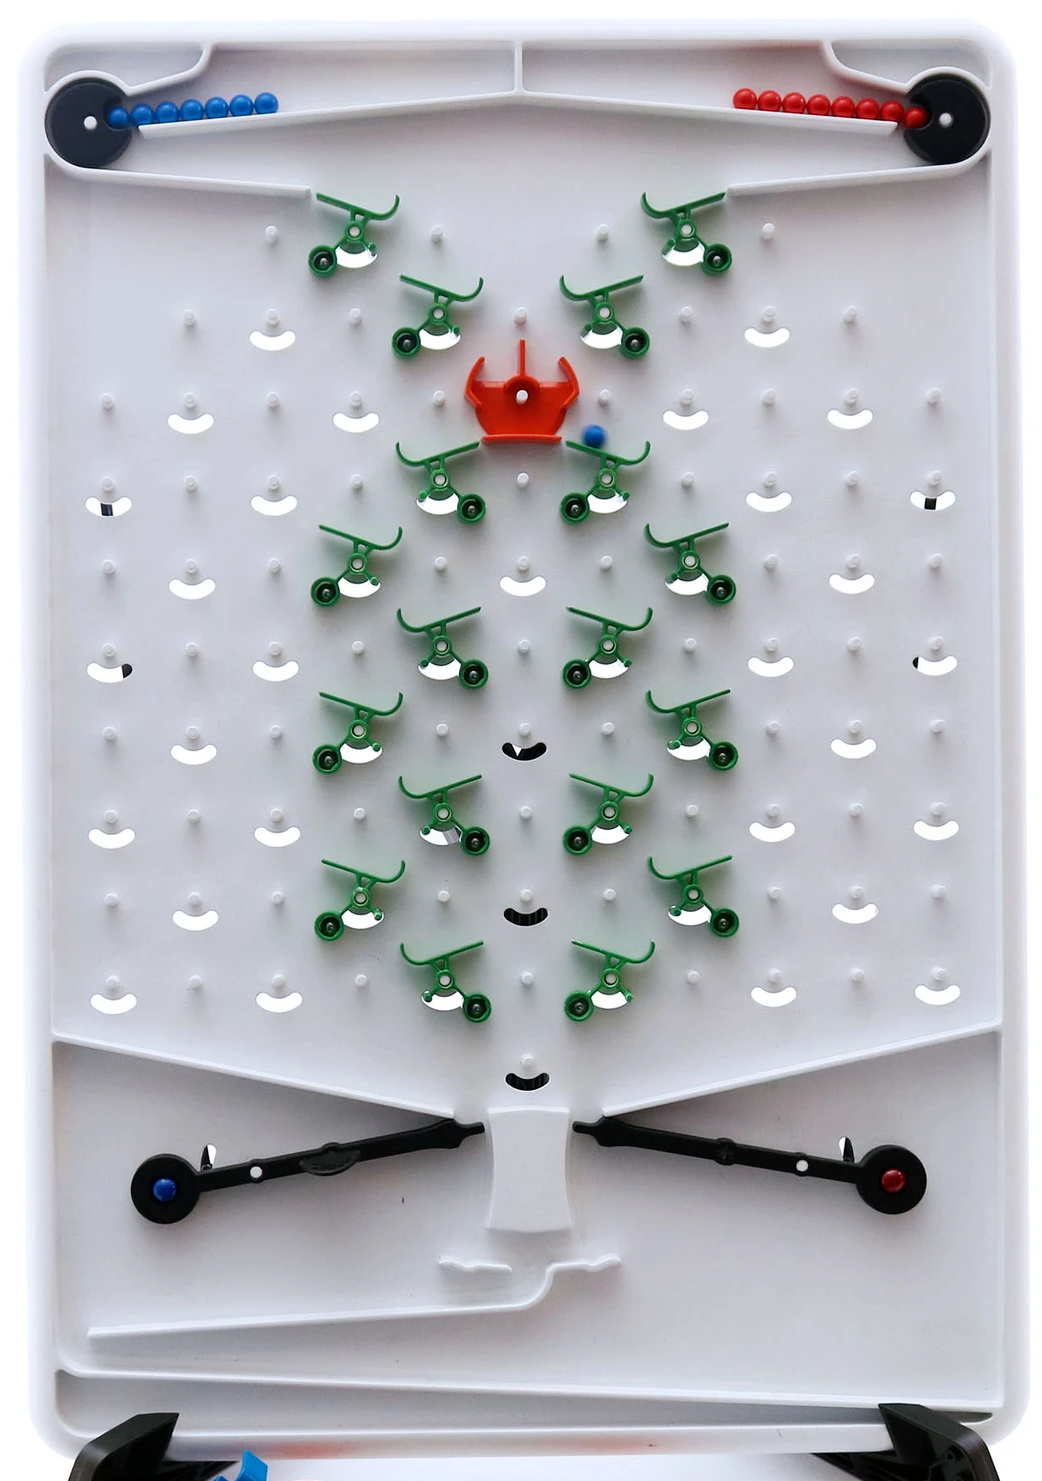
\includegraphics[width=0.6\linewidth]{images/turingTumbleBoard.png}
    \caption{A physical Turing Tumble board with pieces placed onto the board. The marble dispensers are at the top left and right corners with the flippers at the bottom. The board is 34.62cm wide and 47.63cm tall. The boards design is implemented in this program. This image was obtained from \cite{turing_tumble_picture}.}
    \label{fig:ttboard}
\end{figure}

\begin{figure}
    \centering
    \begin{subfigure}[b]{0.20\textwidth}
        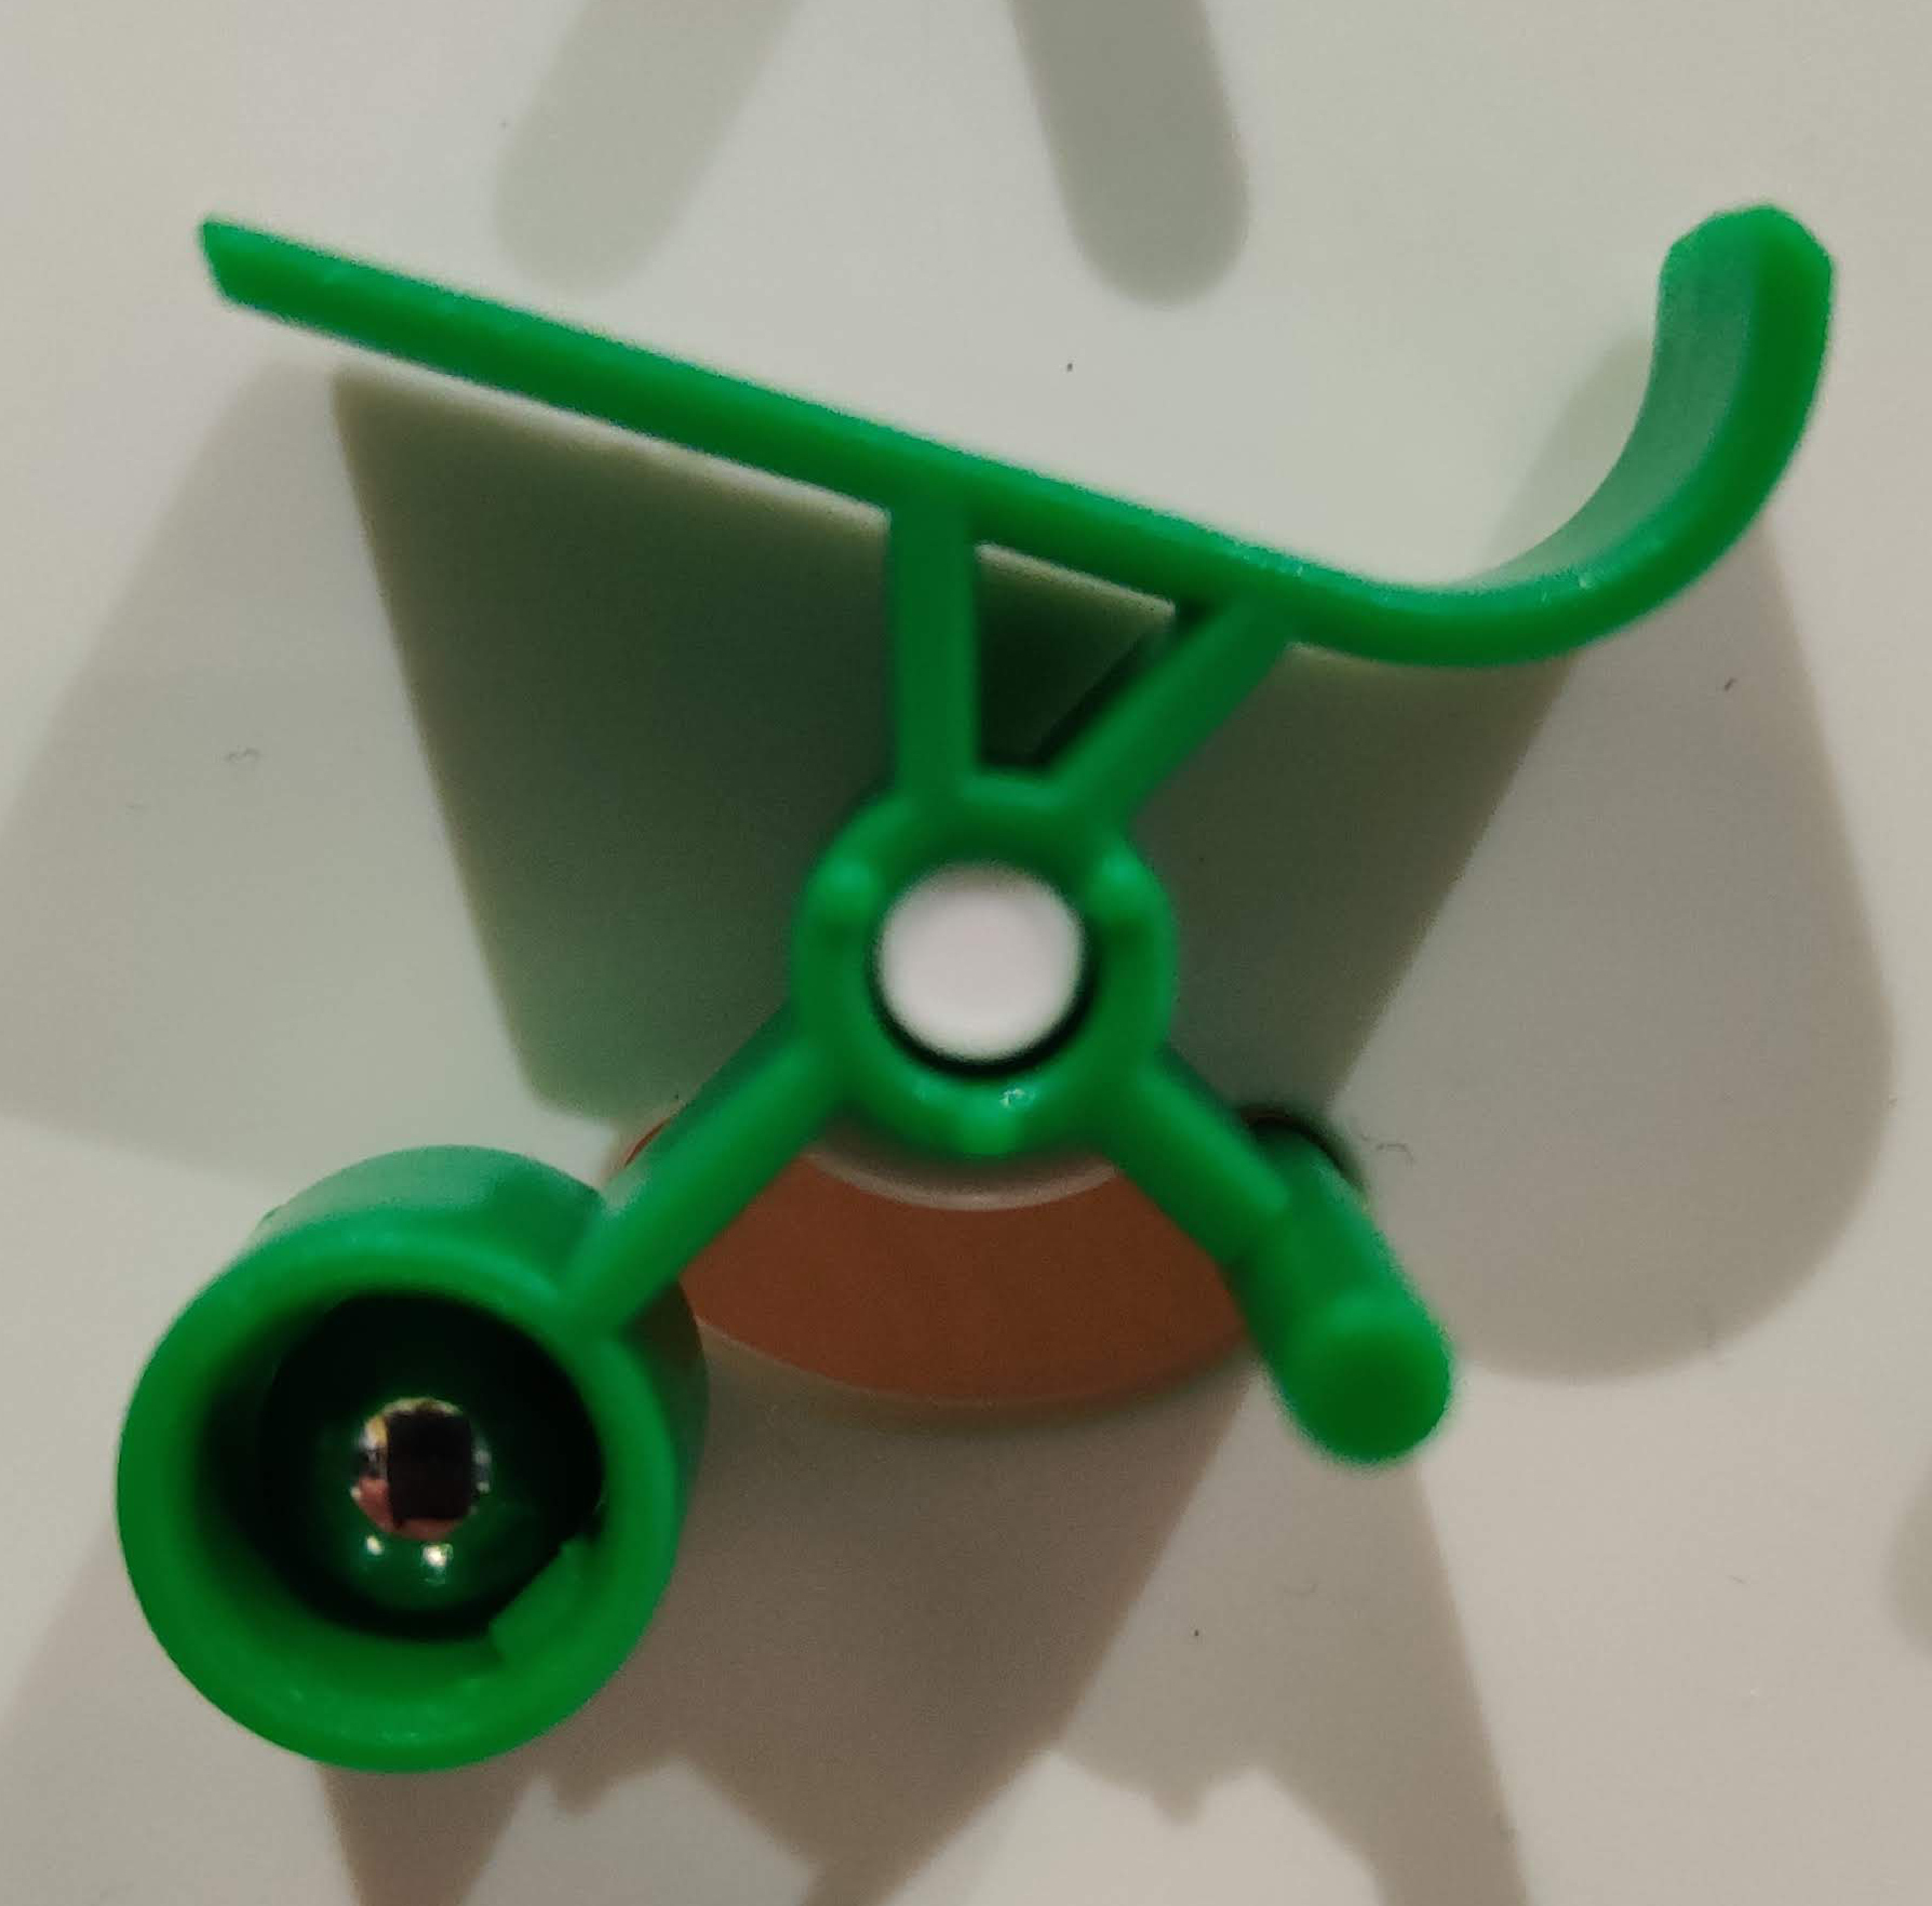
\includegraphics[width=\textwidth]{images/ramp.pdf}
        \caption{A Ramp piece \\}
        \label{fig:phyRamp}
    \end{subfigure}
    \begin{subfigure}[b]{0.20\textwidth}
        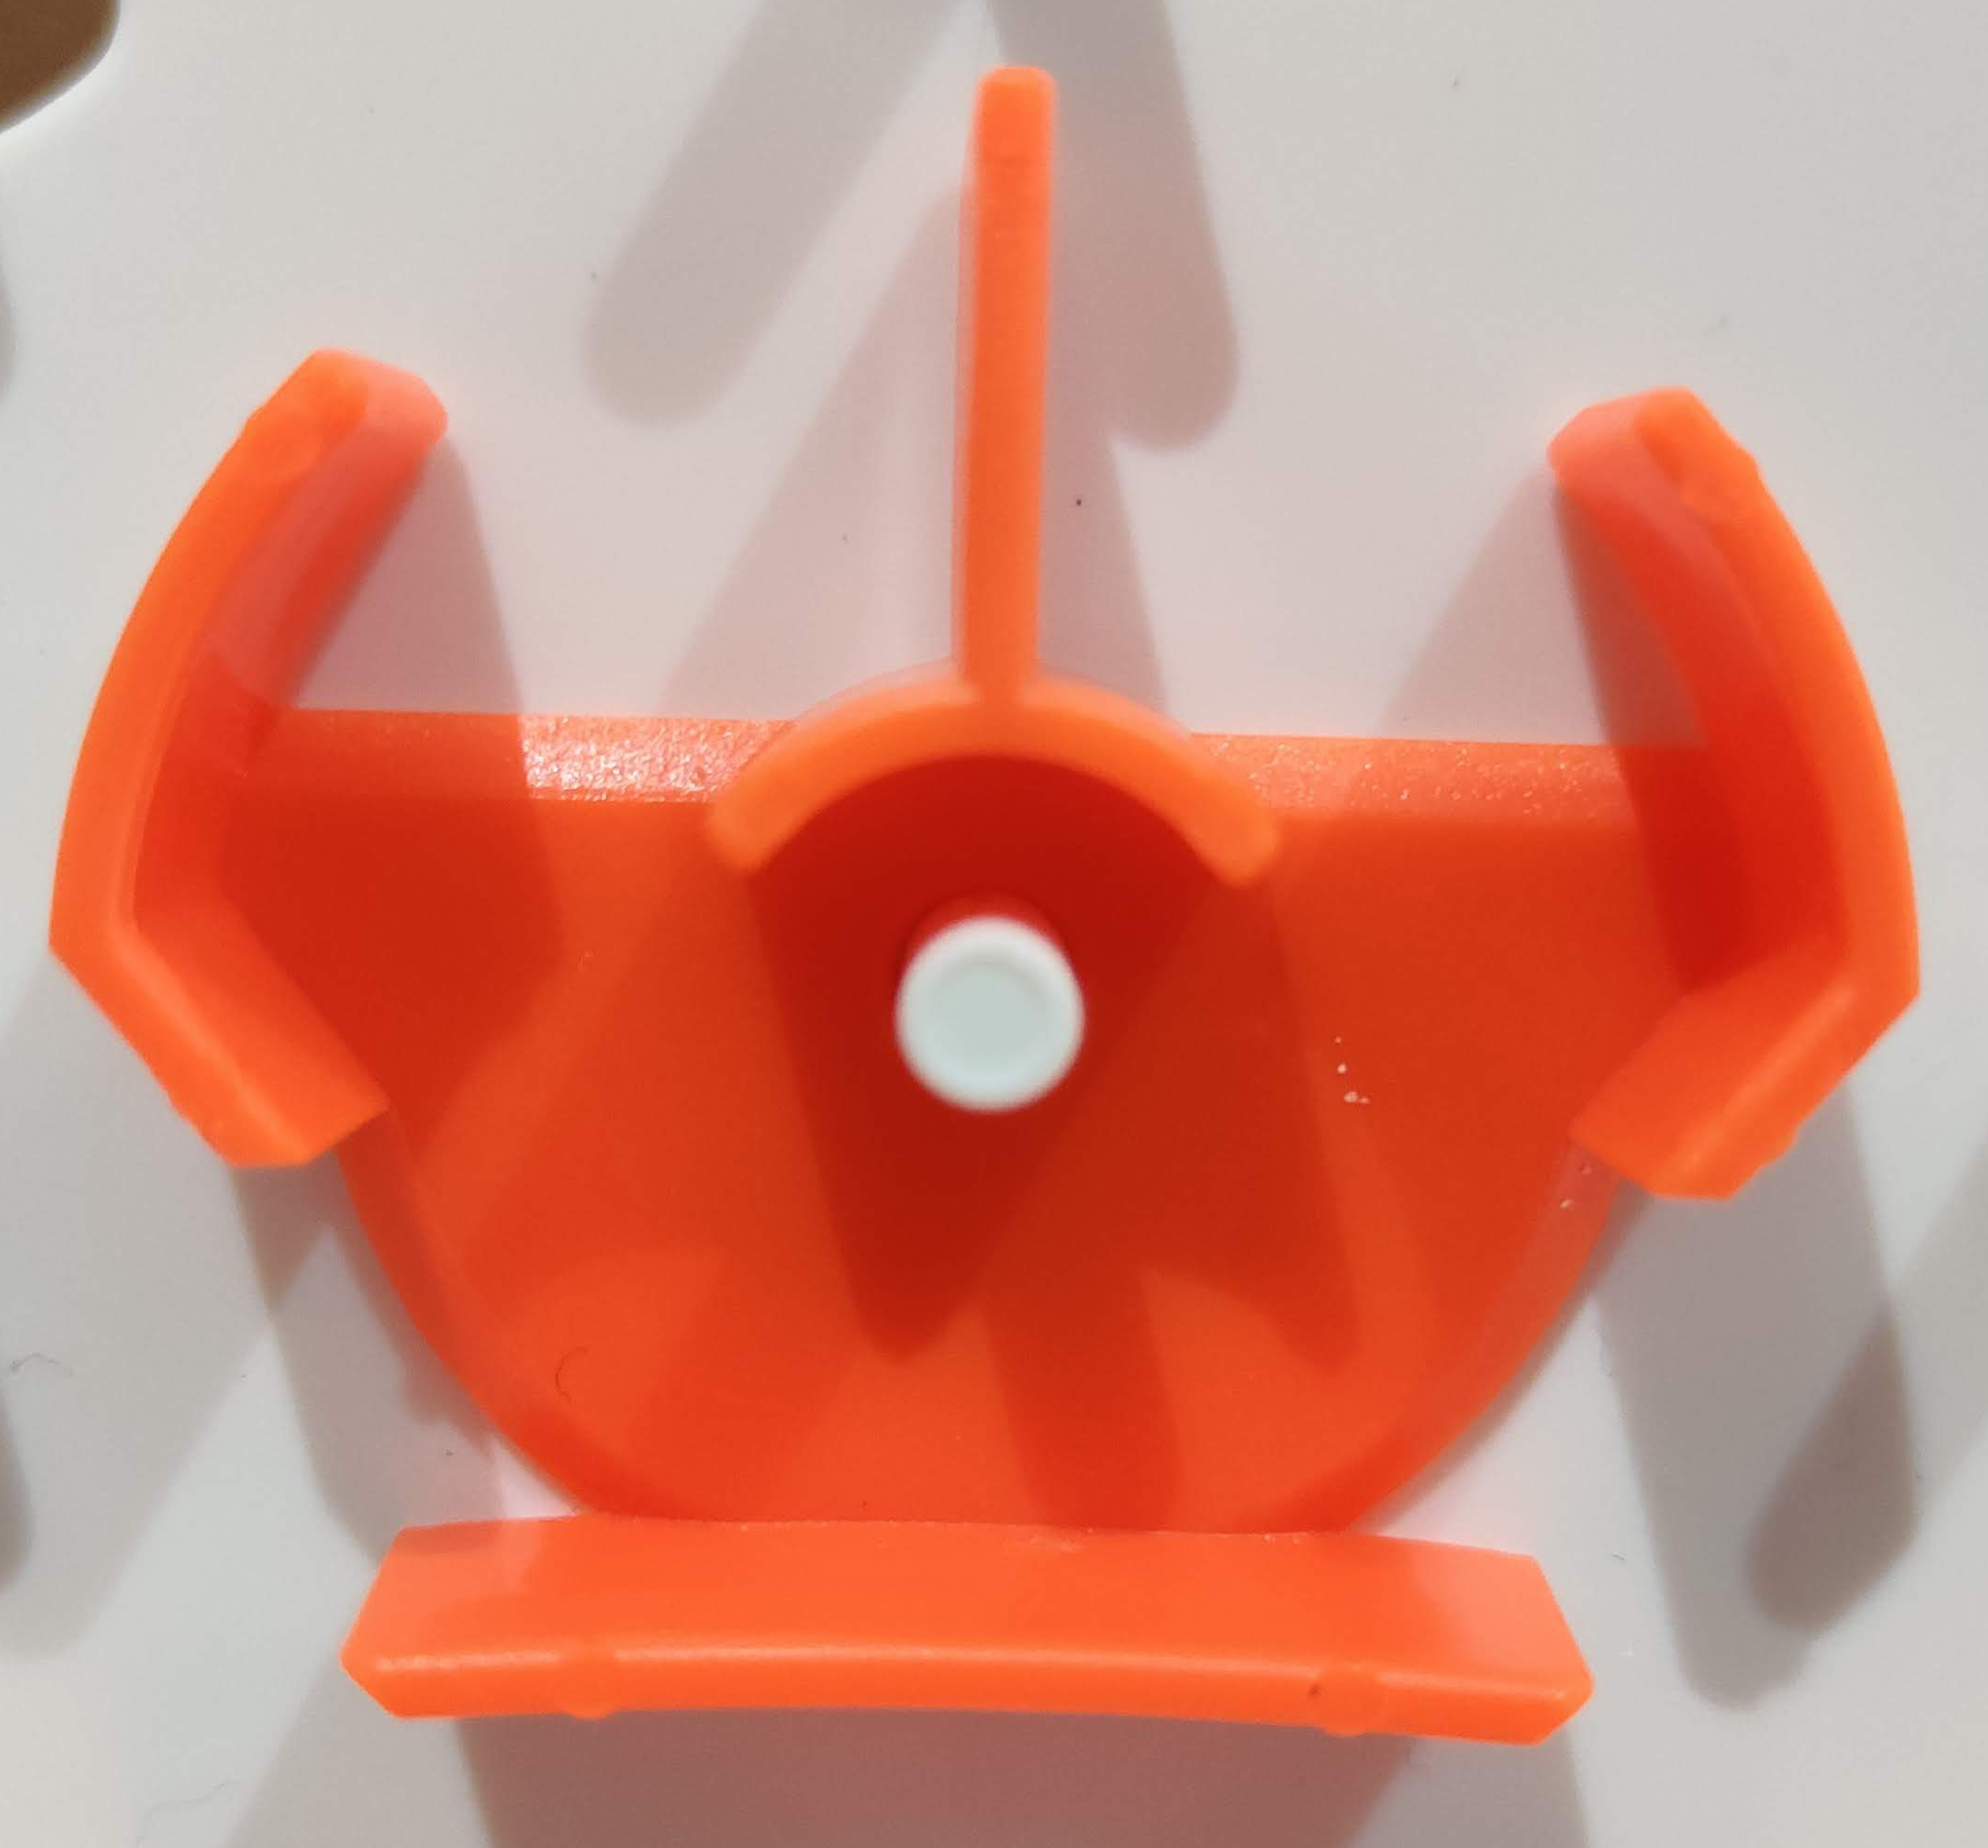
\includegraphics[width=\textwidth]{images/crossover.pdf}
        \caption{A Crossover piece \\}
        \label{fig:phyCrossover}
    \end{subfigure}
    \begin{subfigure}[b]{0.20\textwidth}
        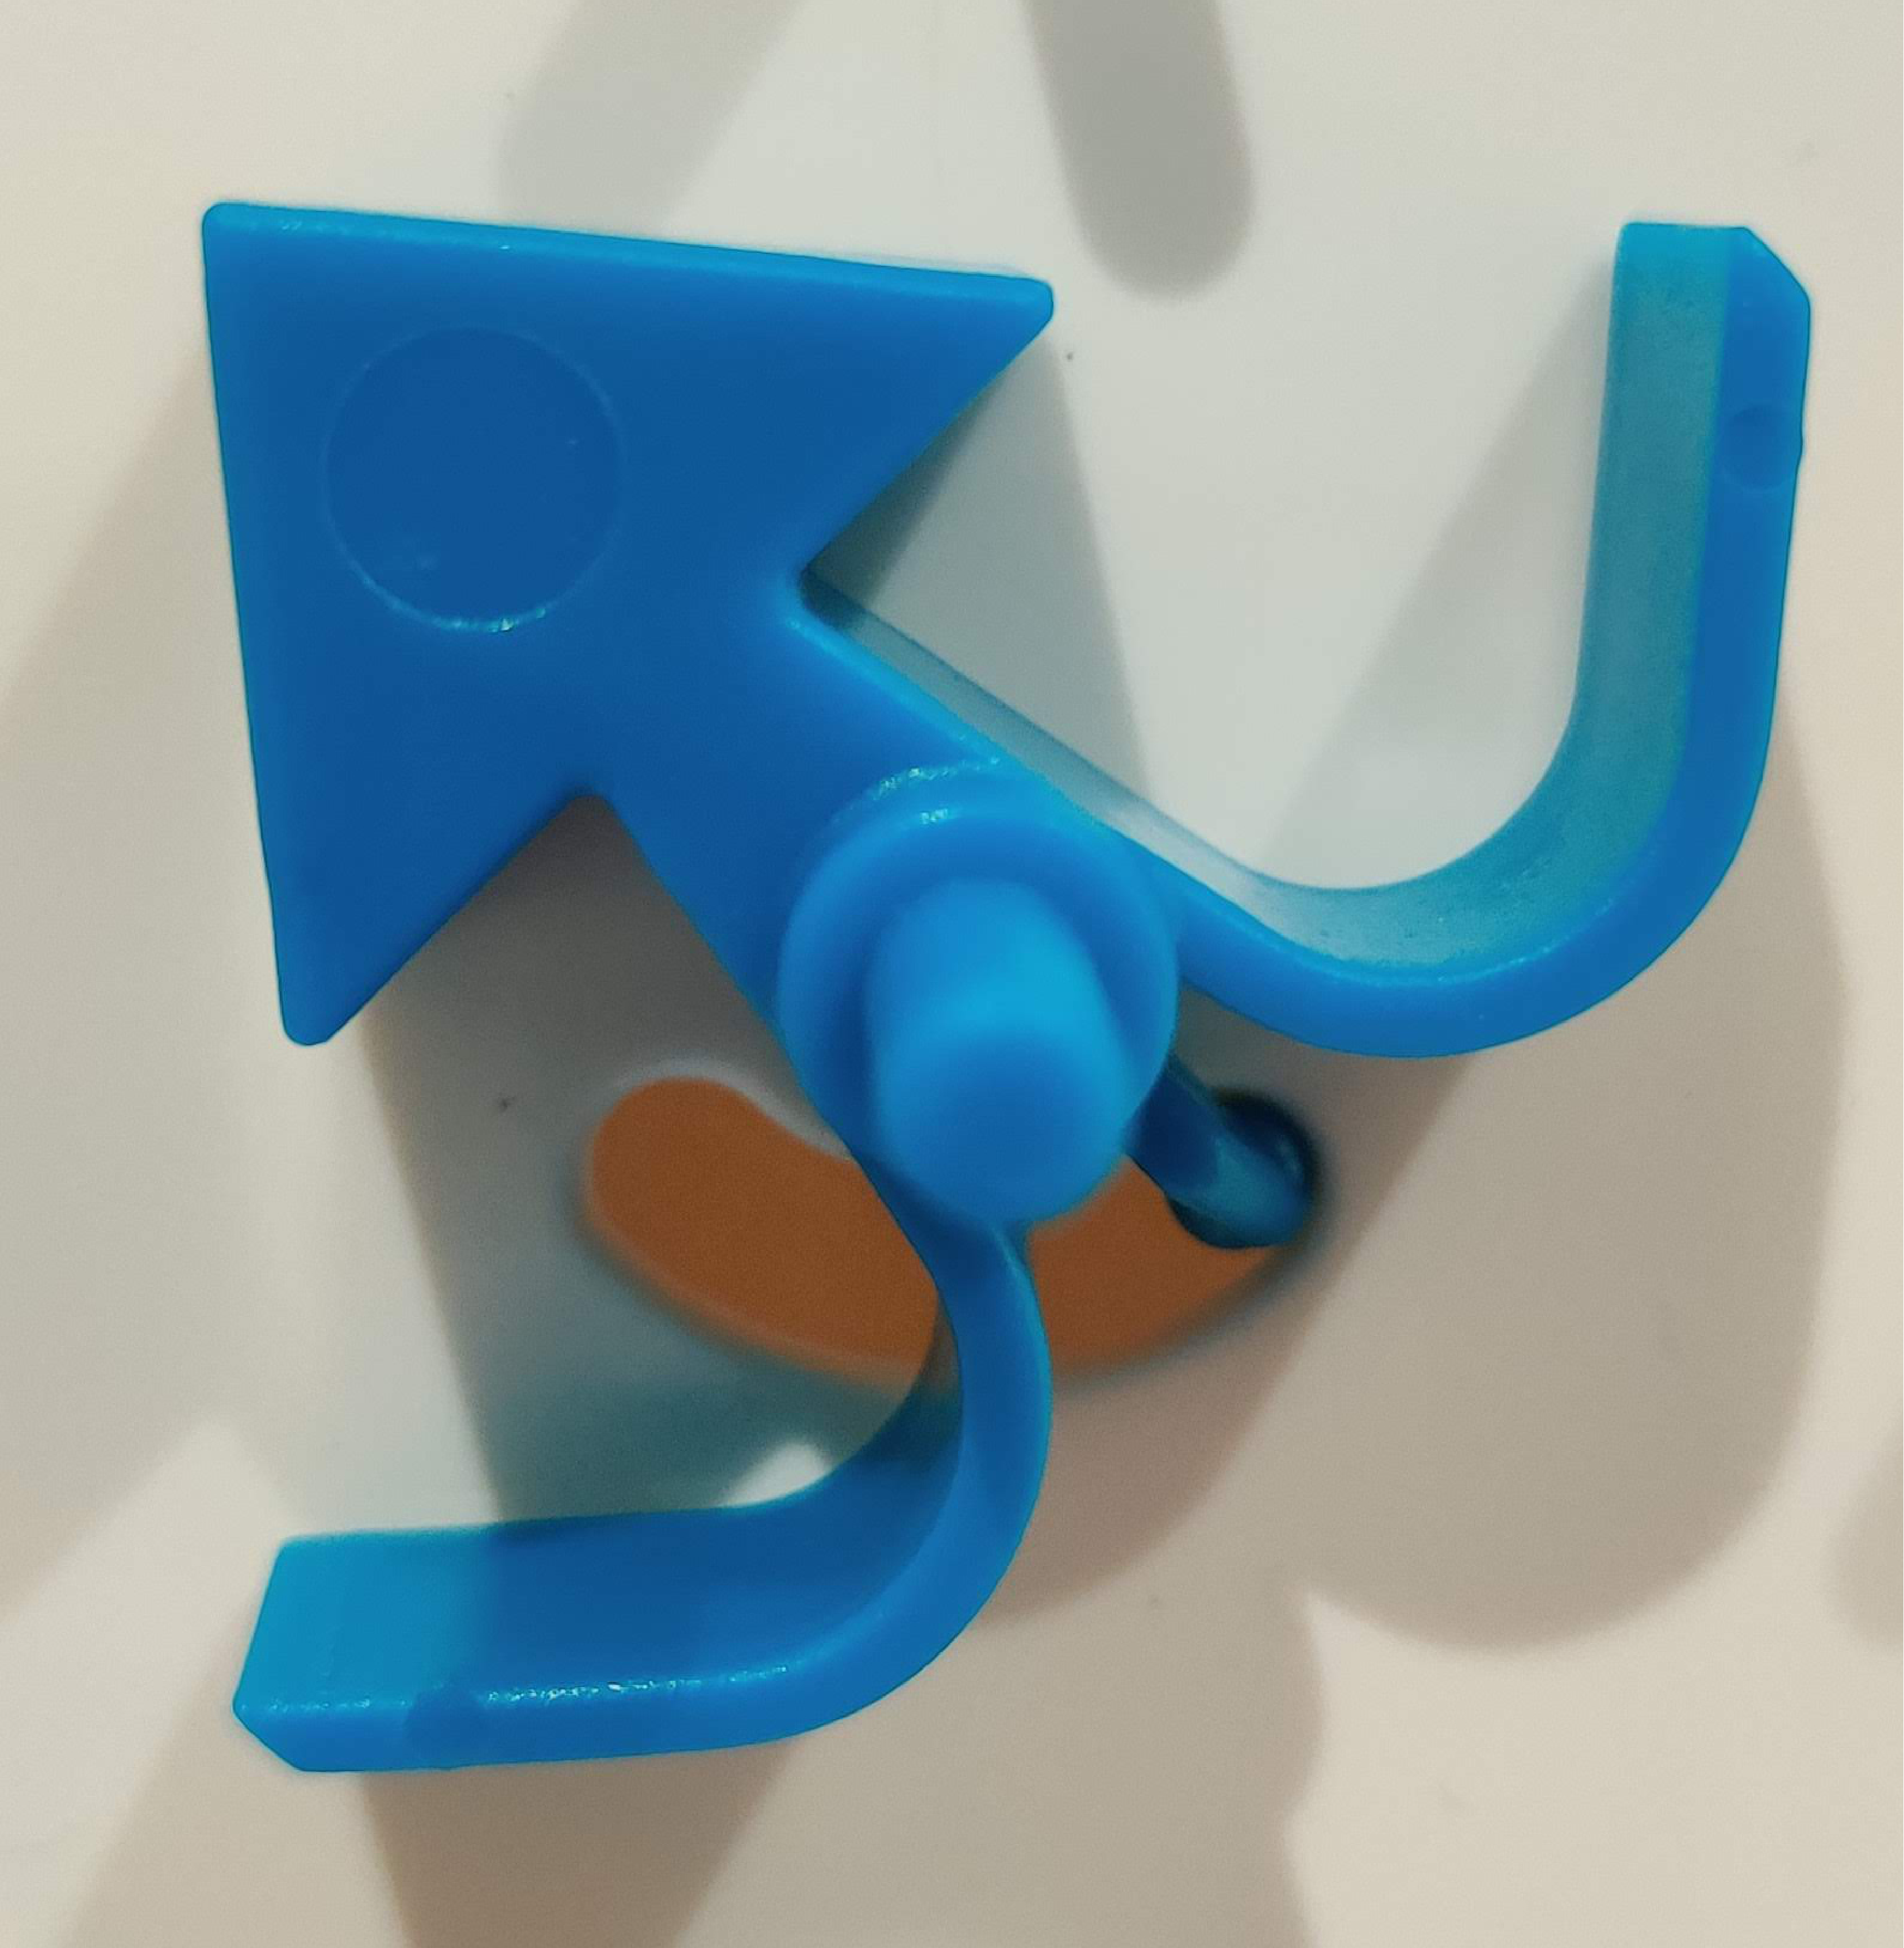
\includegraphics[width=\textwidth]{images/bit.pdf}
        \caption{A Bit piece \\}
        \label{fig:phyBit}
    \end{subfigure}
    \begin{subfigure}[b]{0.20\textwidth}
        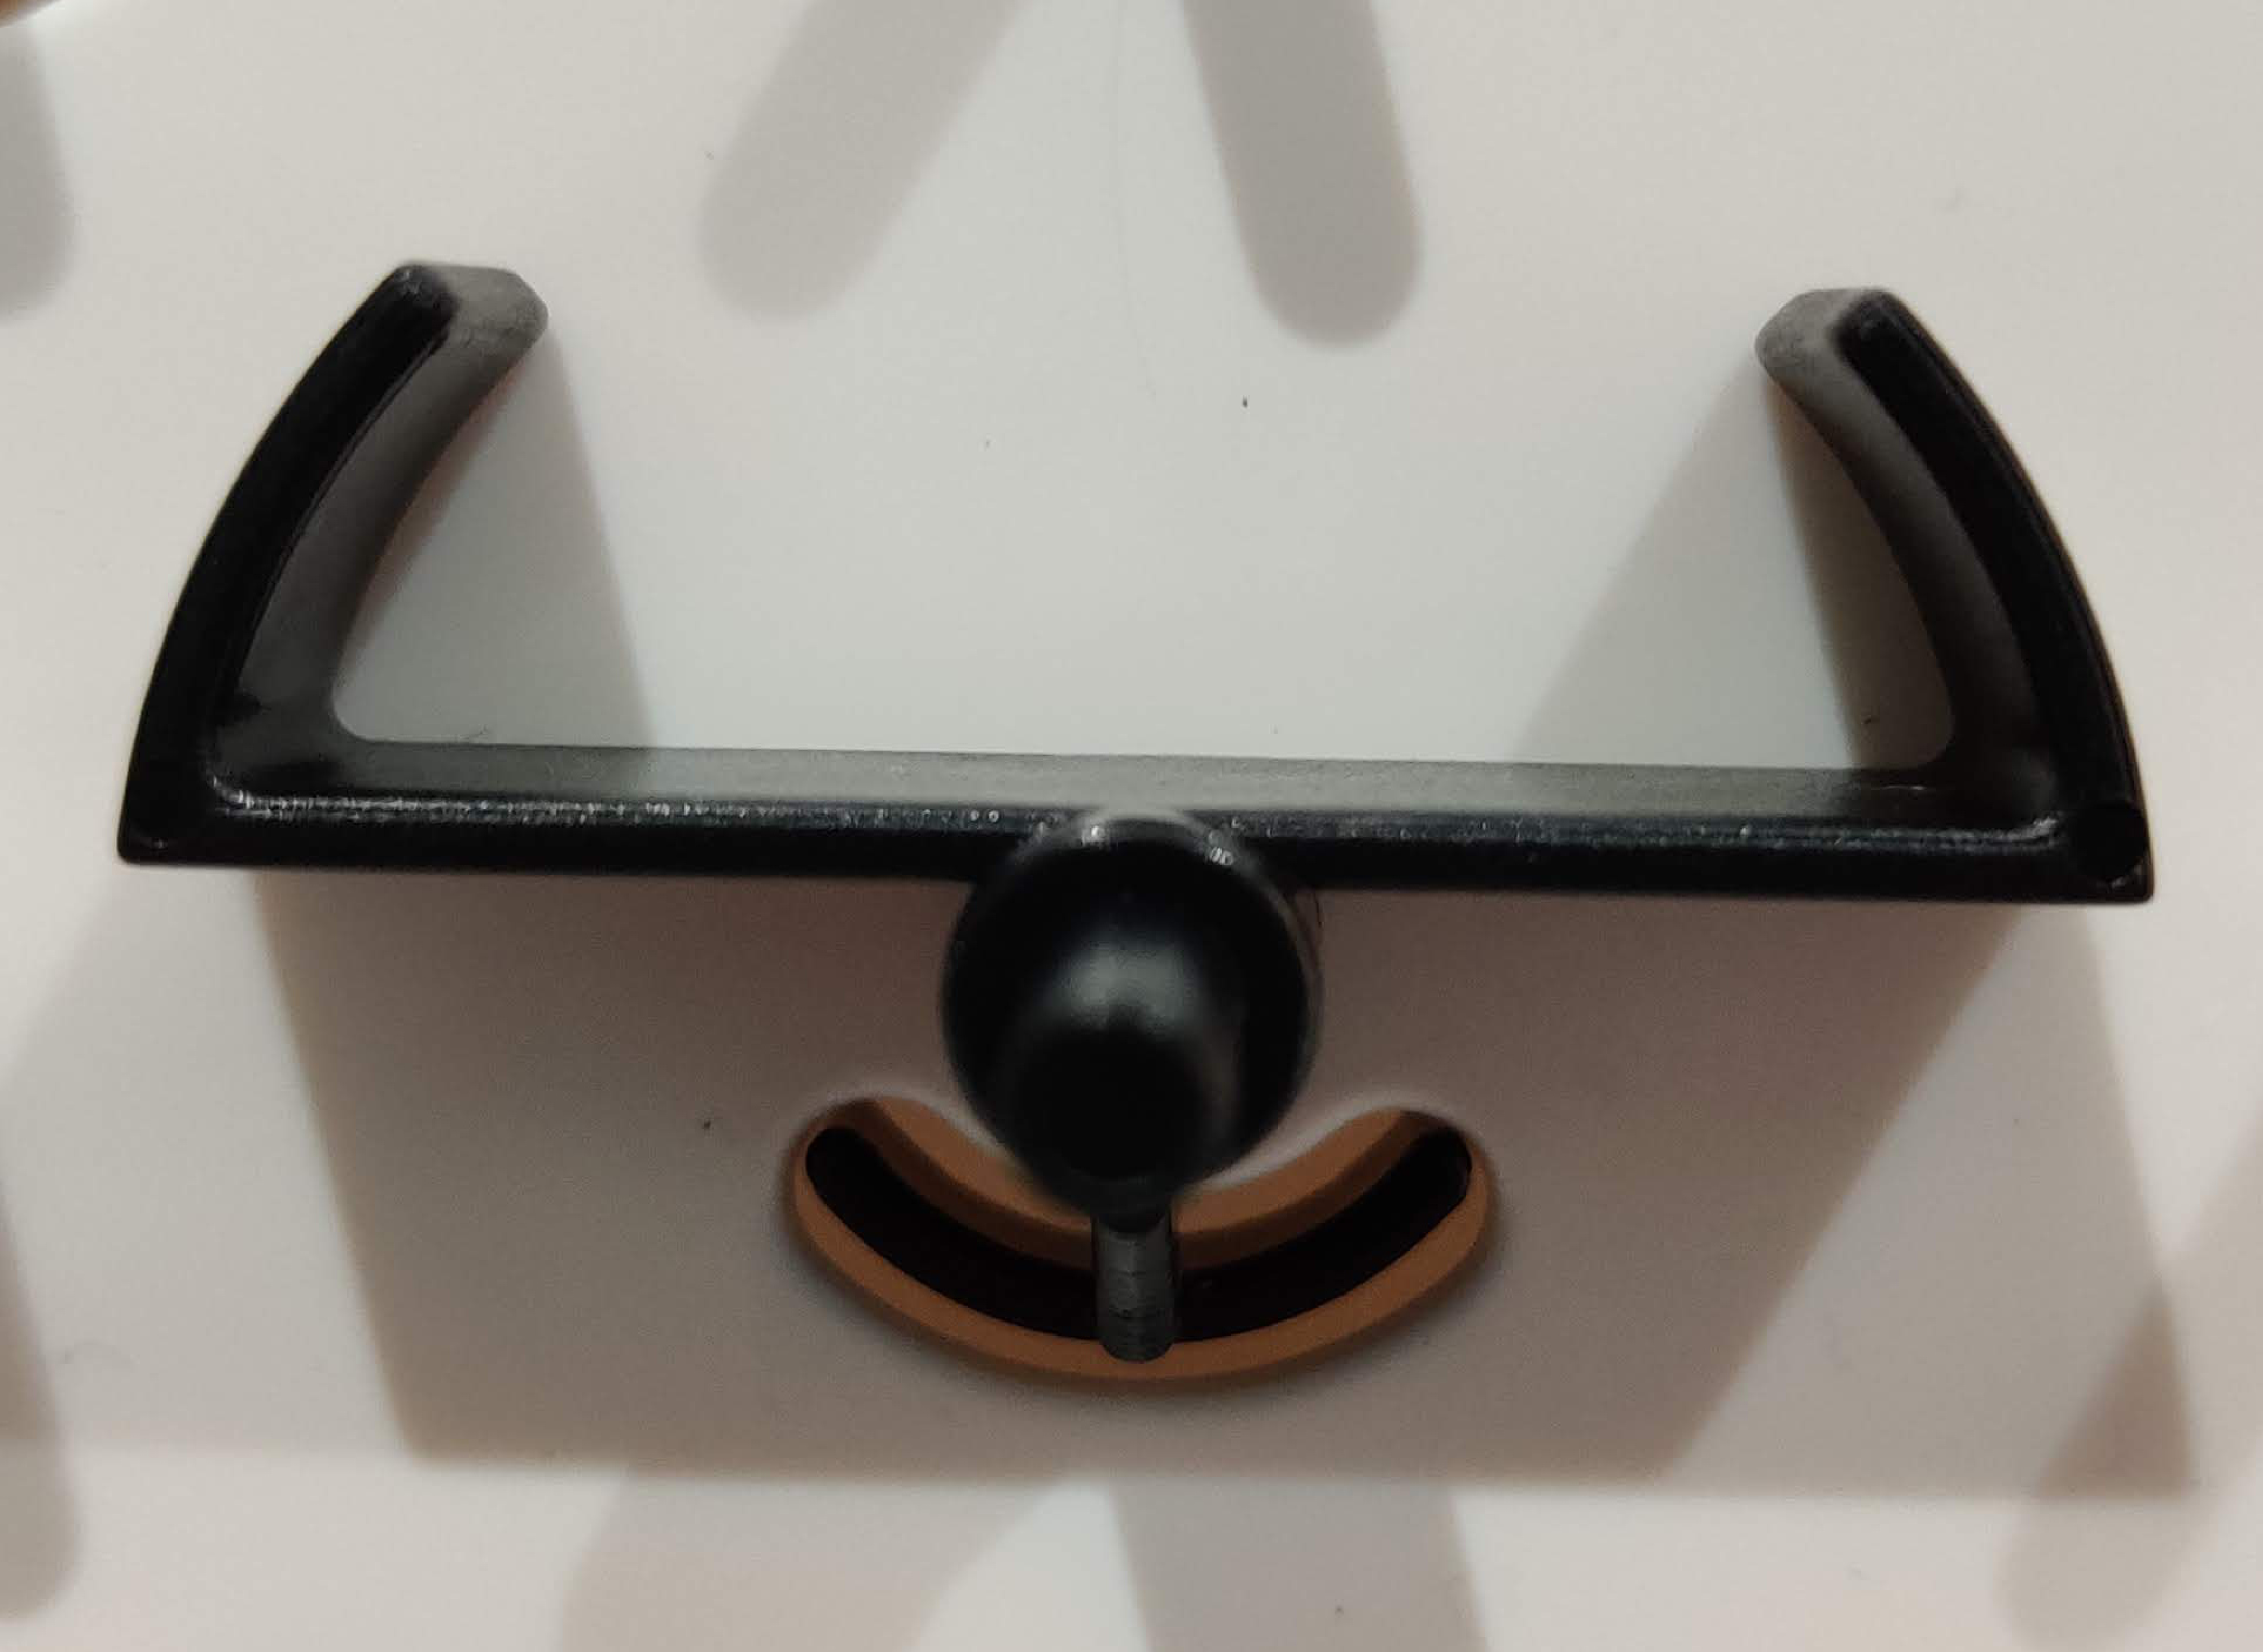
\includegraphics[width=\textwidth]{images/interceptor.pdf}
        \caption{An Interceptor piece \\}
        \label{fig:phyInterceptor}
    \end{subfigure}
    \begin{subfigure}[b]{0.20\textwidth}
        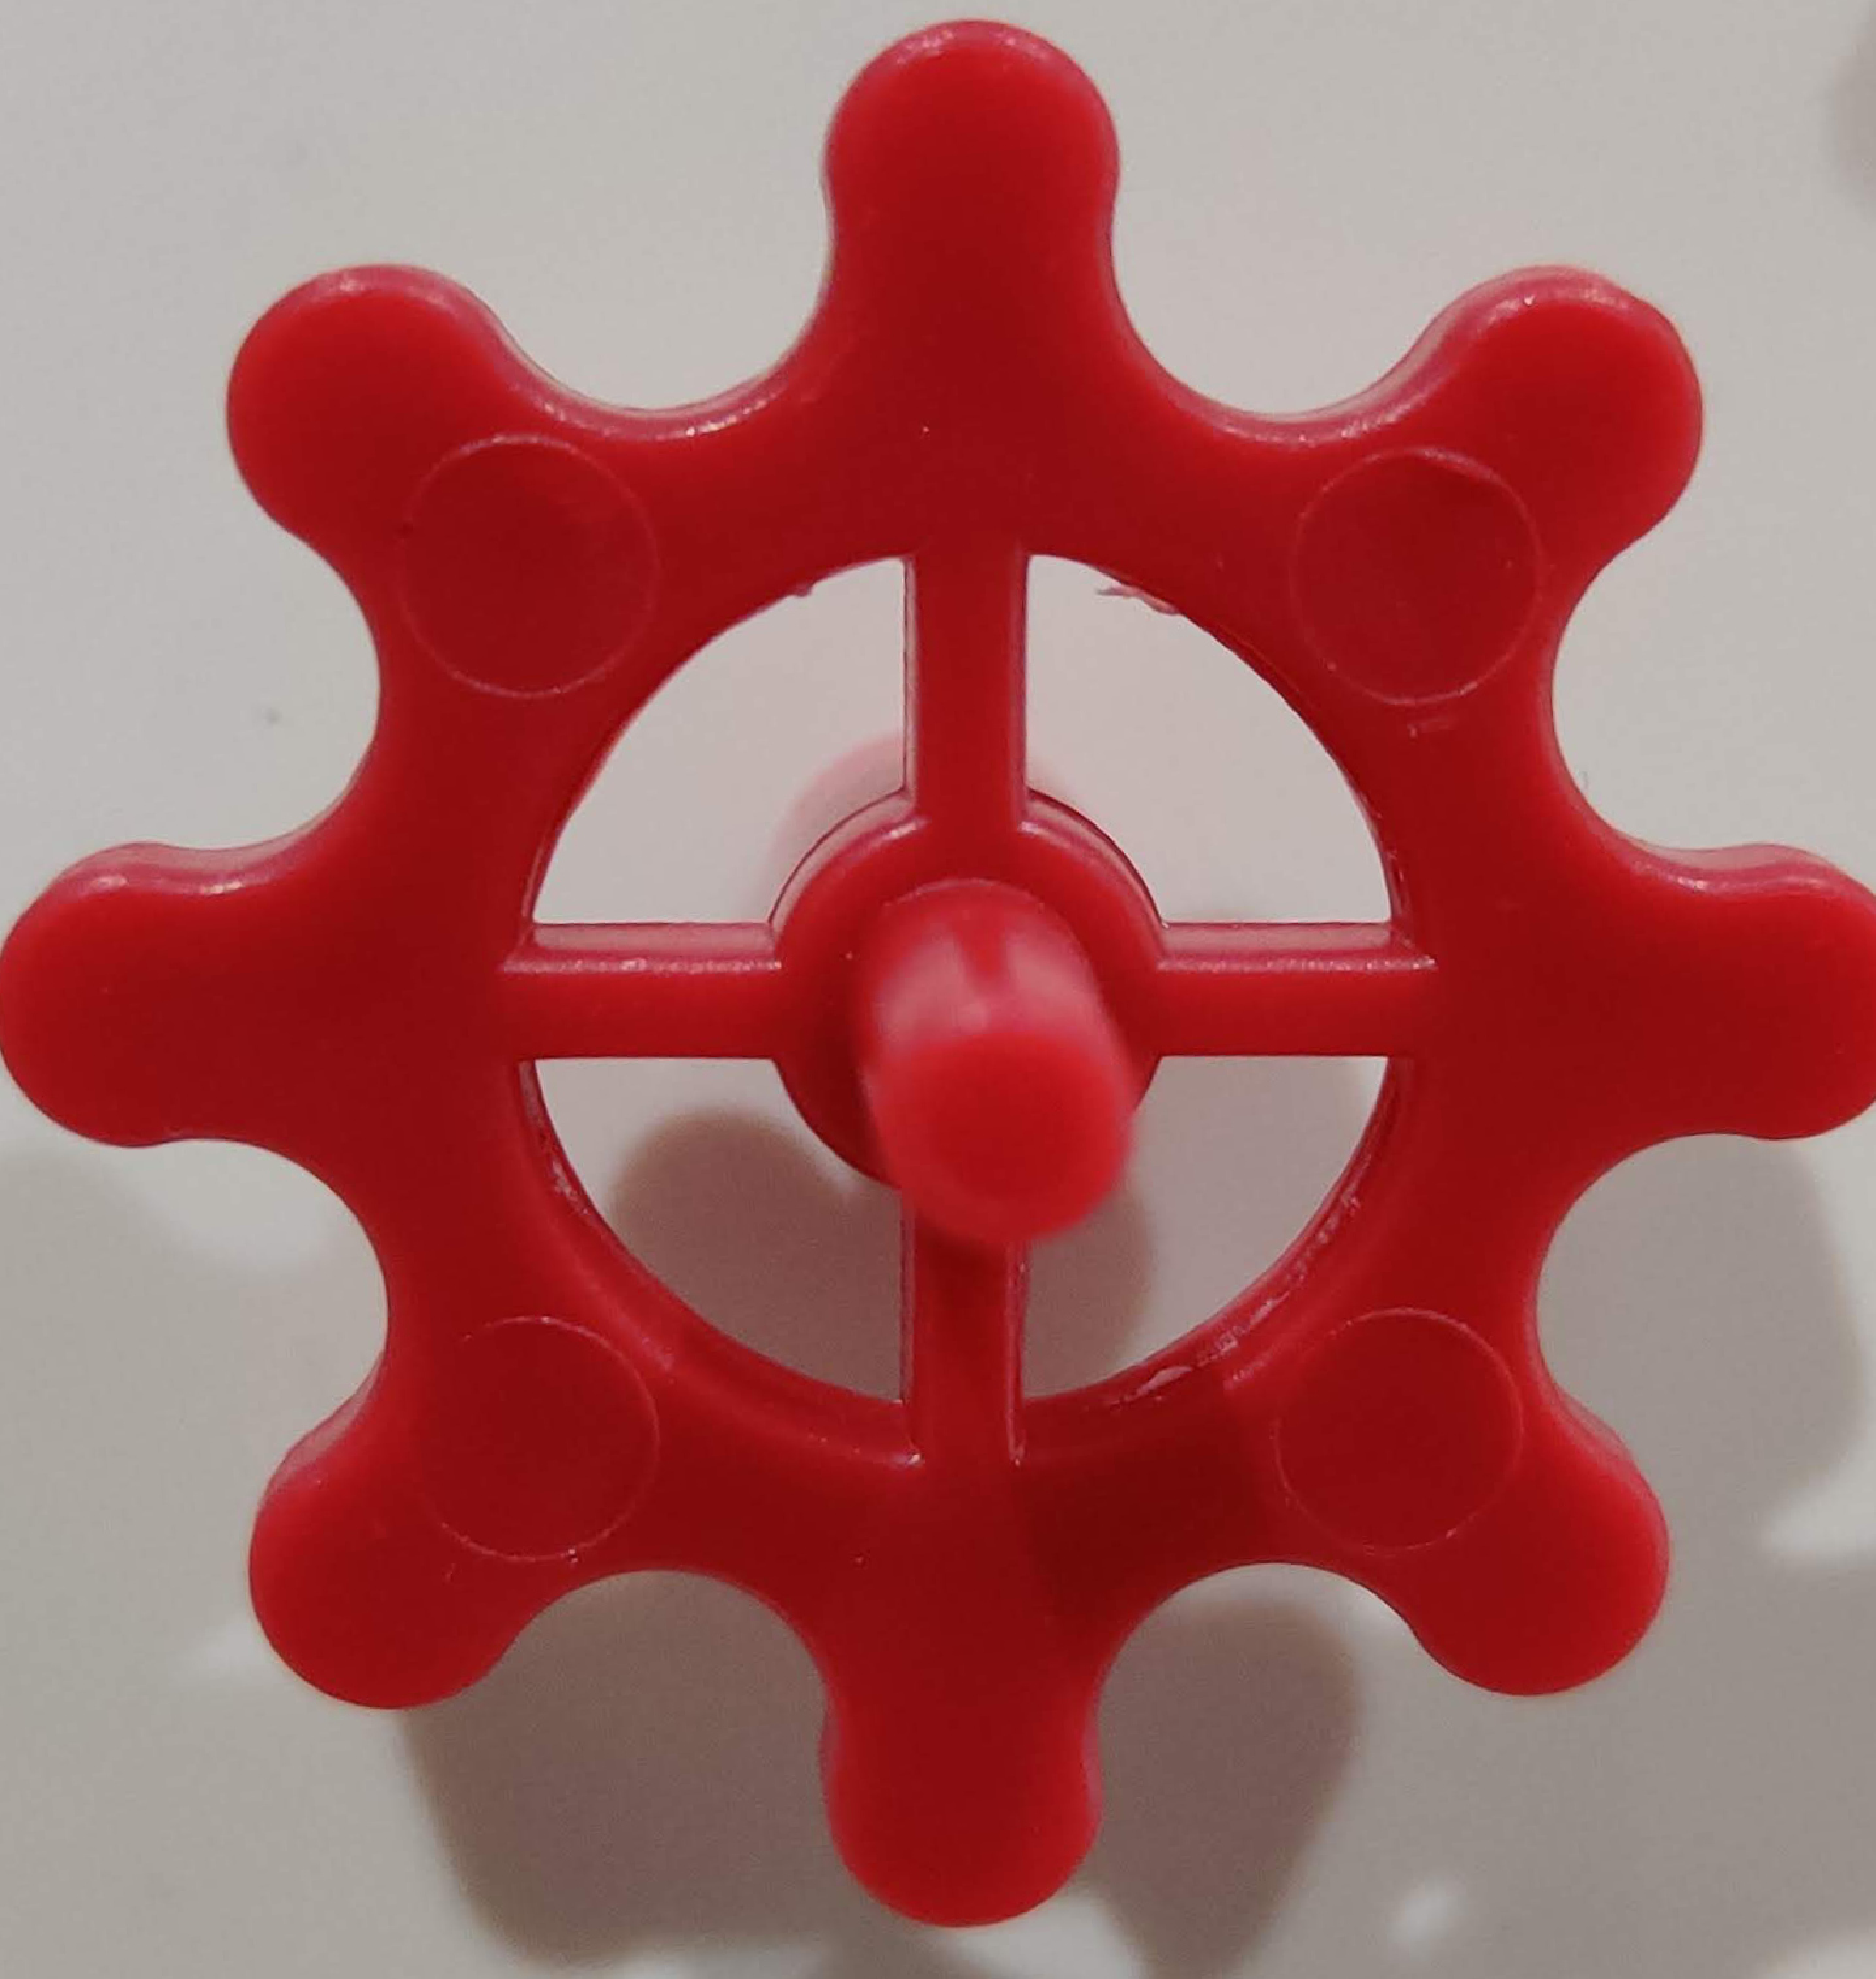
\includegraphics[width=\textwidth]{images/gear.pdf}
        \caption{A Gear piece \\}
        \label{fig:phyGear}
    \end{subfigure}
    \begin{subfigure}[b]{0.20\textwidth}
        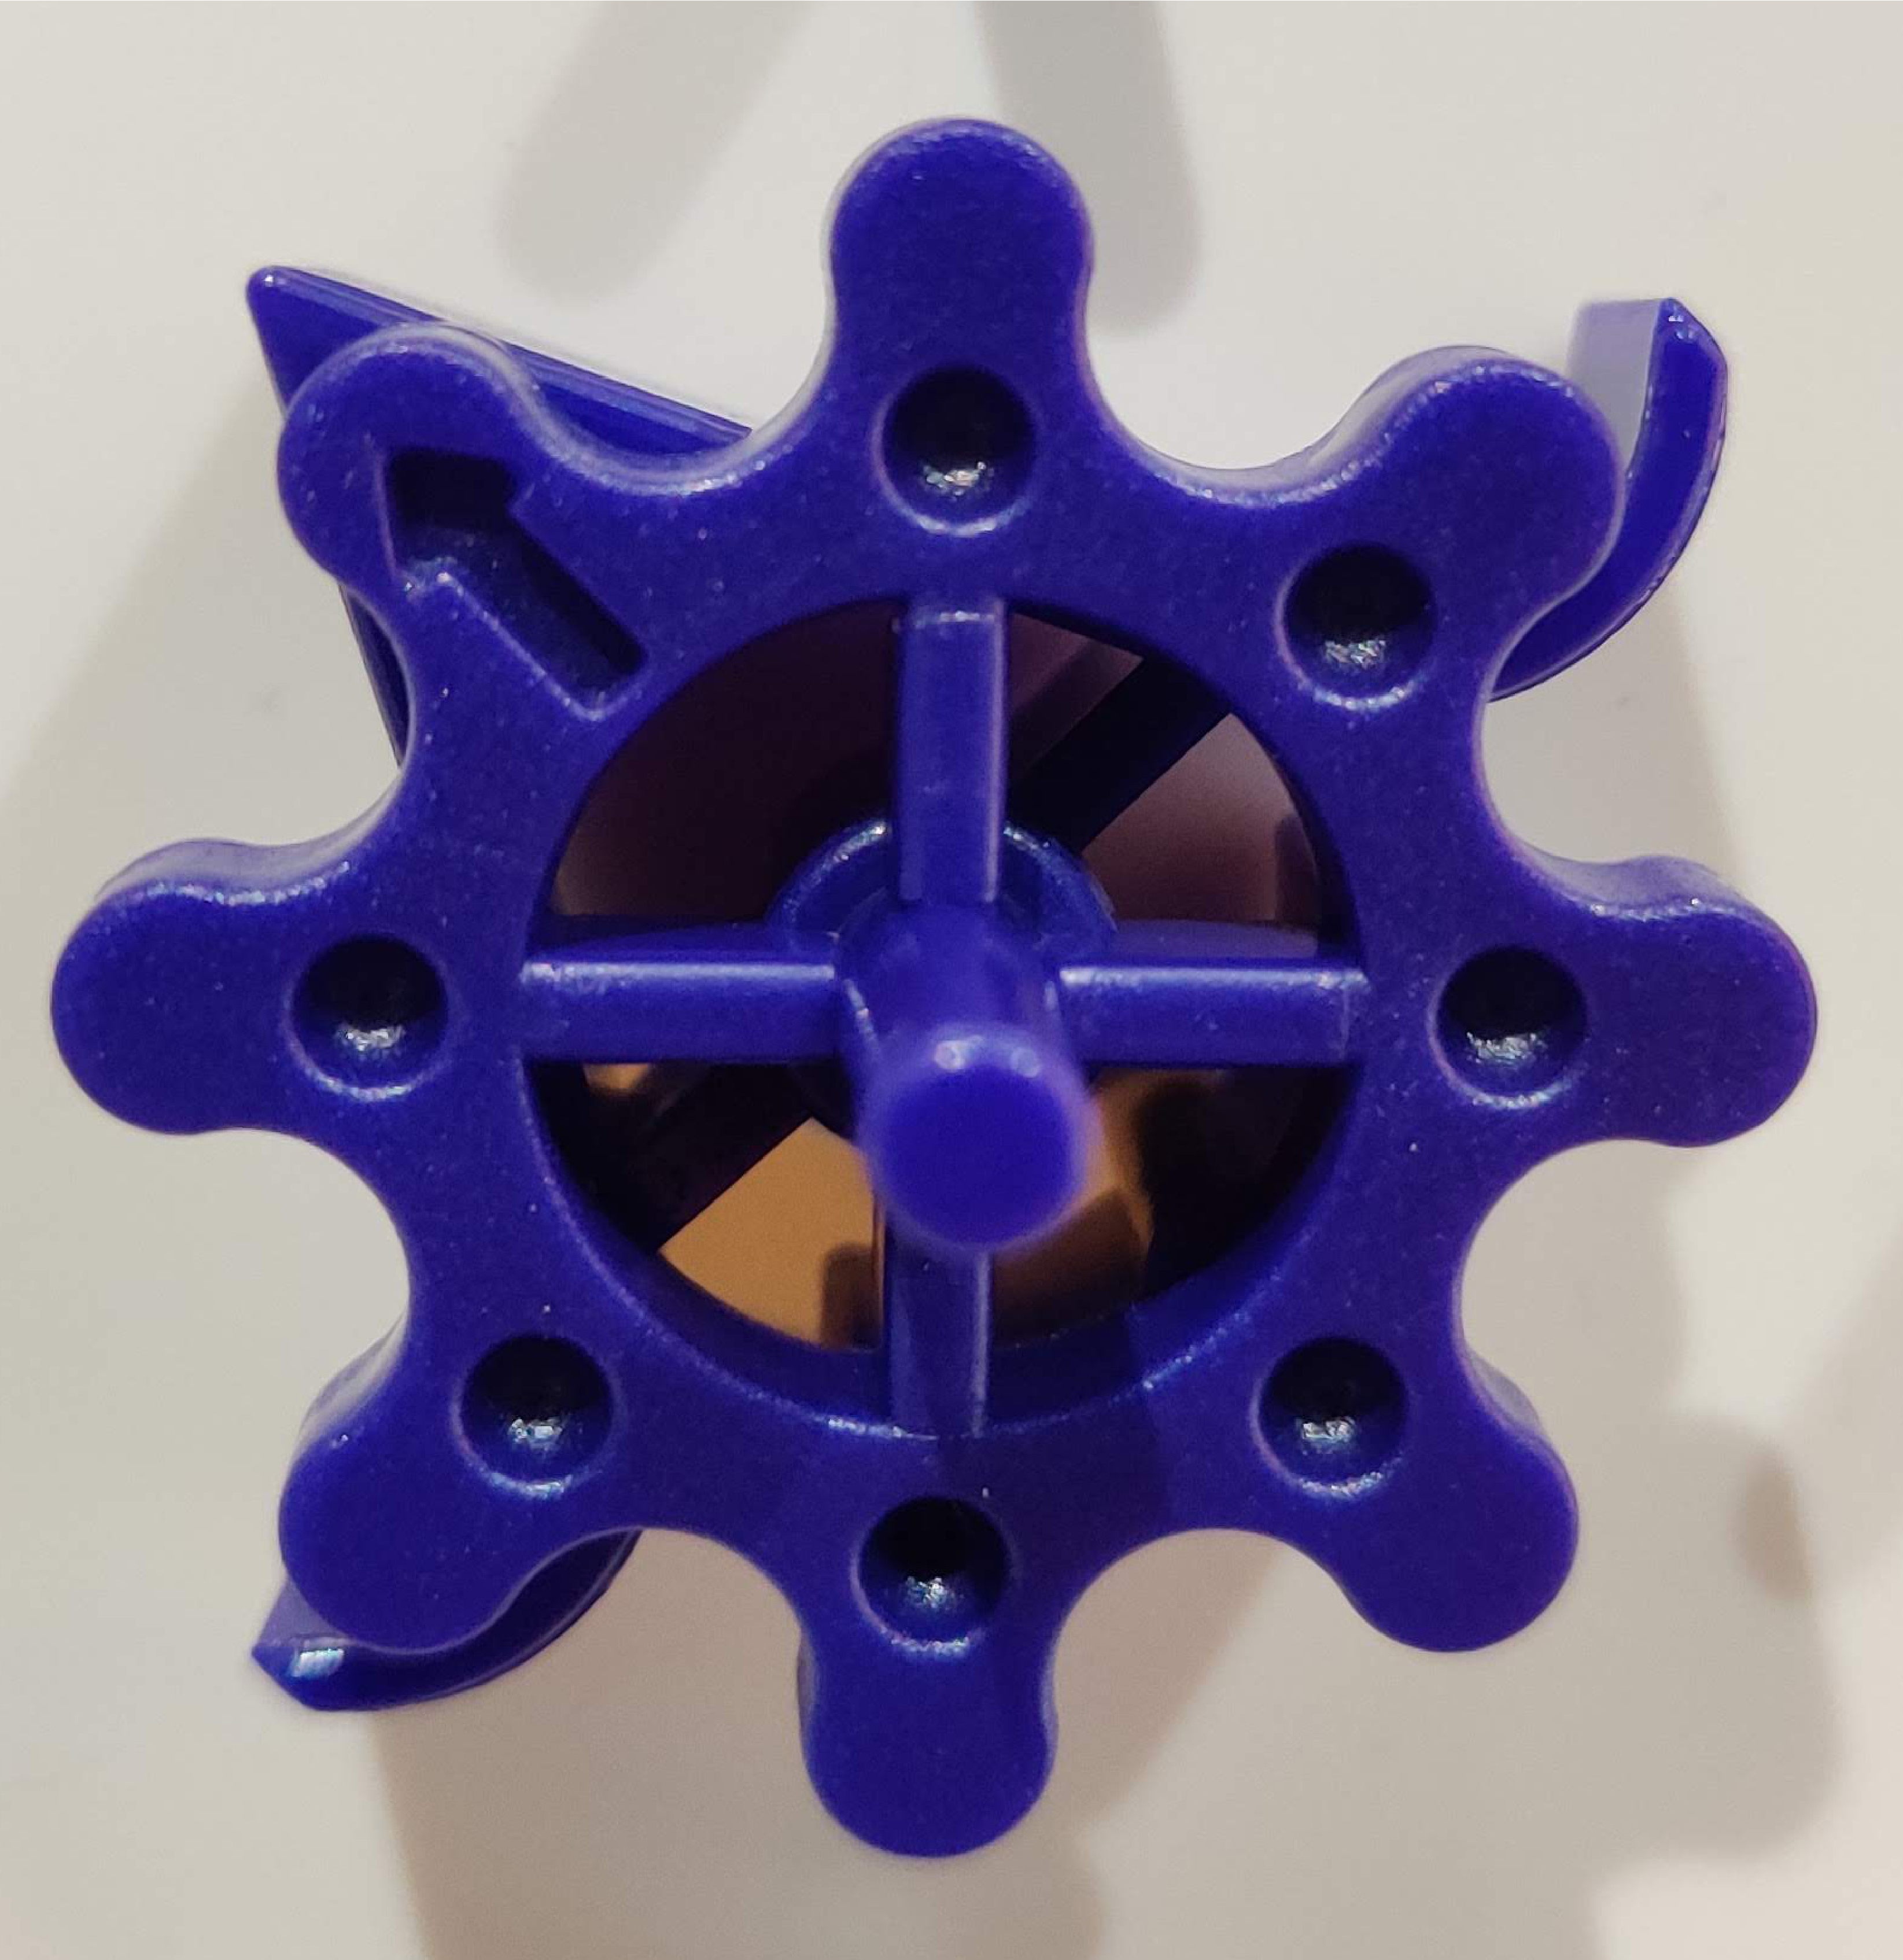
\includegraphics[width=\textwidth]{images/gearbit.pdf}
        \caption{A Gear Bit piece \\}
        \label{fig:phyGearbit}
    \end{subfigure}
    \caption{The 6 different component types (pieces) in the physical Turing Tumble.}
    \label{fig:physicalPieces}
\end{figure}

\begin{figure}
    \centering
    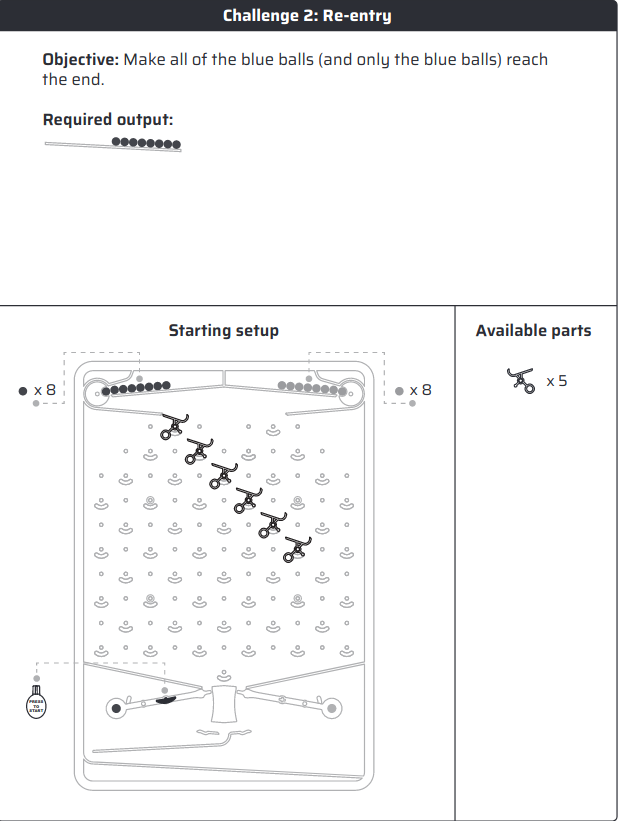
\includegraphics[width=0.5\linewidth]{images/puzzleExample.png}
    \caption{A Turning Tumble puzzle, with a title, description, required output, starting setup, and available parts. Image obtained from \cite{educator_resources}.}
    \label{fig:puzzleExample}
\end{figure}


\section{Existing Turing Tumble Simulators}
In this section we describe existing Turing Tumble simulators and analyse each of them.

\subsection{Overview}
Various Turing Tumble simulators exist online or as downloadable programs. Three such programs were explored and analysed. A paid version was found that implements the board in virtual reality but as this product and implementation style would be unaccessible for the majority of the target audience it was not evaluated. The products were analysed based on the goals set for the project and helped define the requirements for the program.

\subsection{Turing Tumble Simulator}
Turing Tumble Simulator is an open source simulator running in a web browser and hosted on Github pages. (\cite{turing_tumble_simulator}). It was created in Typescript using Javascript libraries for graphics and gravity simulation. 

\textbf{Advantages}
\begin{itemize}
    \item The gravity simulation is impressive and gives a clear and intuitive simulation of the logic of a physical Turing Tumble. Including when marbles fall and interact with the different pieces.
    \item Marbles are simulated correctly when falling down the board and allow complicated configurations to be simulated.
    % \item Extra marbles can be easily added to the dispensers and are collected at the bottom of the board. Unlike other simulators where the number of marbles is represented by numbers, in this implementation it is clearly represented by a graphic for each marble in the dispenser, similar to how it would look in the physical game.
    \item A tutorial page has been added to give clear descriptions of how the pieces and the application works.
    \item The board layout can be edited by adding new walls, slots, dispensers, and flippers giving a large amount of possible customisation options. This can allow users to fully explore the computational power of Turing Tumble by giving more space to add complex configurations.
    \item The board has different speed options to control the speed of the marble falling down the board, helpful to improve a users understanding of how the pieces are interacting with the marble.
    \item An option to change the graphical representation of the pieces can be activated to change the pieces into a simpler view, in which the pieces are represented by a simple graphic showing the direction the marble can go.
    \item Users can download a board as an image, which can later be uploaded to the site. This is an unusual implementation of saving boards where normally a text file is used but the image allows the saved version to be easily recognisable.
\end{itemize}

\textbf{Disadvantages}
\begin{itemize}
    % \item There are only two pages on the simulator, with no clear direction for a new user unfamiliar with a Turing Tumble. This can lead to some initial confusion to a user unfamiliar with Turing Tumble and why they should be interested.
    \item No puzzles can be played on the simulator. This can lead to a lack of an external motivator for users to play with the simulator instead relying on them needing an internal motivator of wanting to learn Turing Tumble without prompt.
    \item To change the direction of a piece, a user must first place a piece then select the 'hand' tool to click on this piece to change its direction. It is unclear why the hand tool would be necessary to change the direction of a piece while also being inefficient to change the direction of newly placed pieces.
    \item When too many marbles are collected at the bottom of the board, they are shown as being on top of each over. This reduces clarity in terms of the final marble pattern, which is the goal of the game.
    \item The tutorial page doesn't describe how Turing Tumble works and may be insufficient for a user unfamiliar with the game to understand.
    % \item Users can't step through a marble path or pause the marble going down the screen so users would need to use the slowest speed to aid understanding of the exact marble path.
    \item Marbles can drop from any height and reach the end of the board and trigger a new marble going against the rules of the physical Turing Tumble.
\end{itemize}

\textbf{Overall}
A very visually appealing simulator that very faithfully simulates how a physical game would play out by integrating complex gravity simulation. Users unfamiliar with Turing Tumble may struggle to understand how to play the game as no clear game instructions exist. There are no puzzles for users, meaning only an internal motivator of an interest in Turing Tumble can motivate users to use the simulator.

\subsection{JS Tumble}
JS Tumble is a Javascript emulator that simulates a Turing Tumble board and is available online \cite{jstumble}.

\textbf{Advantages}
\begin{itemize}
    \item The simulator correctly simulates all Turing Tumble pieces and has a clear graphic for all pieces.
    \item Pieces can be easily placed using a click and place system, with a held piece indicated by a red outline on the selection bar.
    \item A small tutorial text box can be obtained that gets a short description of the board and how to run the simulator. This tutorial is helpful in given users a brief understanding of how to use the various parts of the page.
    \item Users can send the current board configuration to others by sharing a URL with the current board set up. This is useful in helping to foster a community of people to share puzzles with.
    \item Tooltips appear when hovering over options to give a description of their use. Can help make options more clear to users without needing to reread the tutorial page.
    \item The user can temporally store a board in the current browser session to load back at another time. Useful when creating configurations to allow for some experimentation.
    \item The user can step forward and back in the execution of the marble, giving users a great sense of control which can aid understanding.
    \item Four Example boards can be loaded which can show users more complicated and sophisticated configurations helping them understand the computational power of the board.
\end{itemize}

\textbf{Disadvantages}
\begin{itemize}
    \item It has a simplistic user interface and does not react to changes in browser height or width. This may put some users off as it may appear more outdated than the other versions available.
    \item The user can't easily switch the direction of a piece on the board, they must click the piece with the correct direction on the selection board before placing. This can lead to a slower placement of pieces compared with other implementations.
    \item The collected marbles can go off the screen when too many are collected. This won't allow users to check the resulting output if they wish to experiment with more complicated configurations.
    \item No puzzles are available for users to play on the site. As puzzles are the main game element for the physical board, it would be helpful for users to play through puzzles to help learn the game.
    \item It is not clear which side of the board would release the next coloured marble. This may lead to confusion for users unfamiliar with the game.
\end{itemize}

\textbf{Overview}
An aesthetically simple but complex simulator that has a variety of useful features for users familiar with Turing Tumble, including the sharing of boards, and examples of more complex configurations. However it doesn't contain puzzles for users to play through and learn the game with and could also lead to some confusion for users unfamiliar with Turing Tumble.

%  Cut this
\subsection{Emtumble}
This simulator written in c++ is a desktop application that can create and simulate Turing Tumble boards of varying sizes. \cite{tomita_oudonemtumble_2020}.

\textbf{Advantages}
\begin{itemize}
    \item The simulator correctly models the board logic and pieces needed to mimic a Turing Tumble board.
    \item All pieces can easily be placed and added via clicking and placing the pieces. This can allow users to easily place the pieces needed for a configuration.
    \item An icon is added at the bottom of the board to indicate that a marble reaching that location would spawn a new marble of this colour. This makes it intuitive for a new user. These icons can also be placed in new locations to custom the behaviour of Turing Tumble.
    \item A speed slider is available for users to choose how quickly the marble falls down the screen as compared to analogue choices in the other implementations.
    \item The size of the board can be increased and edited for greater customisation. This will allow more complicated configurations to be created, allowing the full computation power of Turing Tumble to be explored.
    \item There are very clear and distinctive icons for the different component types. This makes it easy to identify the pieces and increase understanding of how they differ from the others.
\end{itemize}

\textbf{Disadvantages}
\begin{itemize}
    \item There is no tutorial so may be difficult for new users to understand how to use the program and what Turing Tumble is about.
    \item It requires the user to download the program and to have an install library to run the program. This can an issue for some users if they are unable to install new software onto their machines, for example school pupils on school lab machines.
    \item There is no puzzles to help encourage users to play the game and learn the variety of board pieces and the computational power it can achieve.
    \item A user must use the side selection bar to select the direction of the piece they wish to place. This was found to be an inefficient way to place multiple pieces of different directions.
\end{itemize}

\textbf{Overview}
A complex and well made simulator of Turing Tumble that may be unaccessible by some users by requiring an install of the program. The ability to edit the size of the board can lead to higher user customisation and greater possibility of unique and computationally interesting boards. 
%==================================================================================================================================
\chapter{Analysis/Requirements}
\label{section:reqs}
% Talk about how the requirements were split into reqs needed be to be meet to match existing projects and then the reqs added to imrpove upon these projects 


% Talk about adding puzzles as the external motivator to encourage people to use the app, therefore increasing the possiblit that it could be useful in a learning concept

The main goal of this project was to create a virtual simulator of the Turing Tumble game. As stated in the background multiple versions of the game exist so another major goal was to include features to distinguish this program from existing implementations while focusing on features helpful for learning. The problem was researched by studying Turing Tumble and the existing simulators to develop a set of functional and non-functional requirements. New requirements were later added after user evaluations in which useful suggestions were given that would improve the program for the target audience.

\section{Requirements}
To meet the main goals as described in the introduction, a list of requirements were created which are listed below with their MoSCoW \citep{noauthor_moscow_nodate} prioritization tier. The first main set of requirements were created to match some of the functionality found in other implementations. The second set of requirements were added to include functionality to distinguish this program from the existing simulators and aid learning using the program. Puzzle playing and creation within the simulator were added to met this. The idea was inspired from the physical game which uses puzzles as the main way to play while also helping to teach children how to use the board and create powerful configurations. The set of requirements are split depending on if they required to match the existing simulators or to add new functionality.

The following list of requirements uses the MoSCoW prioritization method to distinguish which features were most important within the scope of the project. 
\begin{itemize}
    \item Must Have (\textbf{M}) - The set of requirements needed for the minimum viable program that can meet the brief.
    \item Should Have (\textbf{S}) - The set of requirements that should be focused on to add value to the program without its success wholly reliant on it.
    \item Could Have (\textbf{C}) - A desirable extra requirement that shouldn't affect the existing project if not achieved.
    \item Would Like (\textbf{W}) - A requirement that won't be delivered due to the scope of the project but are stated for future work considerations.
\end{itemize}

\subsection{Functional Requirements}
\textbf{Simulator Requirements}
\begin{itemize}
    \item (M) Allow users to view, place, and delete pieces on a virtual Turing Tumble board. This should include the 6 piece types present within the physical version as well as the two slot types they are placed in. This will allow a user to build any configuration possible that can be built on the physical Turing Tumble.
    \item (M) Ensure pieces match the logic present in the physical Turing Tumble. The pieces placed by the user should directly match the logic of the pieces in the physical game. This allows the configurations created by a user to directly simulate the physical game.
    \item (M) Correctly simulate the Gear Bit and Gear pieces. These two pieces are required to add Turing completeness to Turing Tumble and should be able to interact with other connected Gear Bits. This will allow the user to create more complicated configurations and puzzles.
    \item (M) Allow users to simulate a valid board. This allows users to play through a Turing Tumble board and understand how the various pieces influence a passing marble.
    \item (M) Add playback features to the simulator. Including a pause / play, speed slider, and a step forward feature. This will allow the user to play at their preferred speed aiding their understanding of the path the marble is taking.
    \item (M) Marbles should be clear and visible on the board. This includes the amount of marbles in the 2 coloured marble dispensers, the marble in play, and the collected marbles at the bottom of the board.
    \item (S) Allow users to save and upload boards as text. The user should also be able to edit this txt file if they wish to edit the board before uploading. This will users to create configurations then save them for future visits to the site.
    \item (S) Create a tutorial page to describe the game and the application. This should allow a user to understand how the application works and how Turing Tumble plays.
    \item (C) Clearly display where a piece can be placed using an opaque piece image before placement. This will help aid understanding of how to place the pieces onto the board. This was a suggestion given during evaluation.
    \item (C) Add a description to each piece type to increase understandability. This will greater improve the usability of the pieces and allow users to learn how the piece works without needing to check the tutorial page.
    \item (C) A user should be able to change the theme of the program. This will add accessibility to the site and allow the user to choose a theme they prefer.
    \item (C) Add a selection of example board configurations to show more complicated configurations and functionality of the game. For example an addition configuration could be added to show how Turing Tumble can use Bit pieces to add two binary numbers together.
          % \item (W) Full gravity simulator for the board. This would greatly improve the visual appeal of the game and be a very faithful recreation of the physical game. It would also add to user enjoyment, encouraging greater use of the site and possible learning effects.
    \item (W) Allow a user to edit the size and dimensions of the board. This would allow users to create more complicated configurations and puzzles to fully simulate the computational power of Turing Tumble.
\end{itemize}

\textbf{Unique Requirements related to learning}
\begin{itemize}
    \item (M) Allow users to play puzzles. This includes adding the main descriptors required to understand what the puzzle is about, as discussed in Section \ref{section:puzzle-background}. This will allow a user to learn more about Turing Tumble while providing a fun way to improve logic based problem solving skills.
    \item (M) Allow users to create puzzles. This will allow users to create new puzzles that other users can play. Creating an environment of puzzles that can be played over time.
    \item (S) Users should be able to login to the site. This will allow the site to monitor which user created the puzzle and display the author name on created puzzles.
    \item (S) Have a list of default puzzles for users to play. This will allow users to have a set to play through without needing the online puzzle environment to be very active.
    \item (S) Create a home page. Should give an brief overview to the site and the different pages a user can access.
    \item (C) Allow users to filter puzzles using a difficulty filter. This will give the user greater control of which puzzles they view and allow a greater ease of learning by giving the option to start with simpler puzzles before moving onto more complicated ones.
    \item (C) Allow users to create custom patterns of pieces and save these configurations. This would allow users to create more complicated Gear Bit patterns that they could use in other parts of the program.
    \item (C) Allow users to comment on and rate other puzzles. This will help create a more active puzzle environment where users can encourage each other to create more elaborate puzzles.
          % \item (W) A leaderboard where users completion time for puzzles can be views. This will give an extra environment aspect to complete puzzles for users.
    \item (W) A user page where users can delete or edit their published puzzles. This will encourage users to create puzzles and update older puzzles with any possible fixes or edits.
\end{itemize}

\subsection{Non-functional Requirements}
\begin{itemize}
    \item (M) No existing knowledge of Turing Tumble should be required to understand and use the program. As this program is decided to introduce people to Turing Tumble, it must be easy to use for this target audience.
    \item (M) Should be intuitive from the outset without the need to keep going back to a tutorial to understand how to use it. After the first read of the tutorial the User Interface (UI) elements shouldn't need more explanation and should be easy to understand.
    \item (M) Should be runnable on browsers with no software install required. This will allow school pupils and Computer Science students to use it without the need to install software, which may be unavailable.
    \item (C) Should be quick and efficient to use on most modern desktop devices. Users will be unlikely to return to a website if it is slow and inefficient, keeping the user experience as enjoyable as possible will increase the possible uptake of the site.
    \item (W) Should be runnable on mobile devices. Some users may not have access to a desktop or laptop so making sure the program can run on more common mobile devices could increase the number of users of the program.
\end{itemize}

\subsection{Requirements Discussion}
The requirements and their MoSCoW priorities were updated during the implementation of the project based on the development effort required and its value to the overall project. All Must Have simulator requirements had to be met first to ensure that base functionality of the program was present. More emphasis was placed on puzzle functionality once the main simulation section of the program was completed. Not all functionality found in other simulators were given high priority as the effort required to implement them was deemed too high given the time constraints, so emphasis was placed on adding functionality not found within existing programs. The functionality found in other simulators which hasn't been met has been added to the future work section.

%==================================================================================================================================
\chapter{Design}
% Doesn't need to be in this order, just possible headings
\section{Application Logic}
\label{section:design}
% \subsection{Component design and architecture}
% One important design decision made was to focus on using a component design philosophy to group together related user facing UI code, backend functionality, and styling rules into modular Components that can be called in different locations and can be sent different input values to display different data to the user using the same repeated internal functionality code. This allows for example, a single component to represent the various board pieces, this component can then be given an exact piece as a parameter and represent this to the user but the component can abstract way the exact information of which piece it needs to display.

\subsection{Piece Interface}
The first design decision was how to represent the 6 piece types of Turing Tumble. Each piece would need individual logic in which it would process a marble, changing its direction and updating any internal state, while containing no more information than it requires. It was important to abstract away the logic of the pieces so the board execution algorithm wouldn't need to check the underlying functionality of pieces when executing. A board piece abstract class was designed to contain the properties required to model a piece while containing any methods that would be repeated across all 6 piece types. This included the pieces position on the board, its method to process a marble, and its type. This abstraction of pieces allows the main execution to not require details of the pieces stored in the slots and only have the single responsibility of processing a marble falling down the board.

\subsection{Board design}
A large design consideration involved the representation of the Turing Tumble board. It was decided that a class should be created to store all data related to the board as well as any methods required to update its state, for example the number of held blue marbles. The internal logic of child classes was abstracted away while ensuring the board object had all the data necessary to made boardwide decisions. For example, Gear Bit pieces have internal functionality similar to Bit pieces while the board is responsible for turning any connecting Gears, this ensured that only one class would have this responsibility and a child class wasn't given functions to edit state of sibling or parent objects. The board is the most complex object to simulate so ensuring that there was a single source of truth for the data while making it the only object responsible for the game execution made it easier to design this algorithm and ensure validity of the board state. 

Slots were the main part of the board class that had to be modelled, these were contain the various pieces. An interface design was chosen such that component slots and pins could be abstracted away to ensure that the slots could be separated into the two distinct types without adding development overhead to the board class. A 2-dimensional array representation was chosen for the various slots on the board. The board pattern of 11 by 11 slots leads naturally to the use a 2d array with any slot access operations being easily carried out. 


% \subsection{Playback options}
% 3 main playback options were designed for the board, play / pause, step forward and speed increase / decrease. As a Turing Tumble can be quite confusing for new users, a speed value was designed to be changed by the user so that they could find a speed comfortable for their ability. Pausing execution allows the user to stop the execution of the board to greater understand the processes involved before continuing board execution. A step forward function was designed that would pause execution then move the marble to its next location, bypassing any speed constraint. This gives total control to a user in how quickly or slowly they wish to go through various parts of the board, allowing them to step forward the more trivial aspects or sped more carefully when interacting with a more complicated pattern. No step backwards function was designed as the development complexity of going back through the more complicated Turing compete Gear Bits wasn't seen as a high priority. 

\subsection{Main execution algorithm}
The algorithm responsible for simulating a marbles execution path was designed to loop through a function that calculates a marbles next position. By having a function for a single step, playback controls could then be designed to interact with the looping function rather than adding more responsibilities to the algorithm responsible with a marbles next position. This algorithm validates the marbles position and then uses the hidden internal logic of the current piece to update position and direction. It was decided that when a marble reached a slot that contained no piece it would be seen as an error and a user would need to release a new marble. This was to follow the rules in Turing Tumble where users are discouraged from dropping marbles a great distance between pieces. This would encourage users to skip complicated configurations in favour of dropping a marble to the bottom. It was therefore seen as a more faithful simulation if this was not allowed in this program. 

\begin{figure}
    \centering
    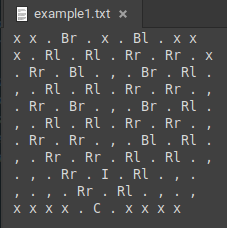
\includegraphics[width=0.5\linewidth]{images/savedBoard.png}
    \caption{An example of a board configuration saved as a txt file, with the pieces and slots represented by characters.}
    \label{fig:savedBoard}
\end{figure}

\subsection{Saved Boards}
To allow users to save copies of boards they create, a text file system was designed. This allowed the board to be represented by an 11 line file that contained a set of characters to represent the slots or pieces on the board, separated by spaces. An example of this can be seen in fig. \ref{fig:savedBoard}. This representation was designed to be easy to understand and edit for a user wishing to create the board using a text input. Each piece is represented by a capital letter with a lowercase letter denoting its direction. The file follows the board layout with its 11 by 11 output allowing an intuitive way to understand a pieces position on the board. While not the only way for users to edit a board in this simulator, it was seen as useful for a user wishing to save multiple copies of boards in an easy to read and edit format.

\subsection{Puzzle Board design}
The design of the puzzles was chosen to follow the puzzle design as discussed in Section \ref{section:puzzle-background}. As the focus of this program is to simulate a Turing Tumble board faithfully, by following the existing puzzle design, it would be recognisable for users already familiar with the game. A board to represent a puzzle was designed to extend the existing board class to ensure any user facing code could accept a puzzle board as data and still display the board to the user without updating the existing user interface. New properties and functions where added to this extended class including the starting set up of a puzzle and the available pieces. By having this new class extend the original, functionality designed for the board execution could be reused by this new puzzle board, saving development time and reducing the responsibilities of this new class. 

\subsection{Puzzle creation design}
The design of the puzzle creation followed the different aspects of a physical Turing Tumble puzzle. A phase system was designed where users would use the existing board and placement features to create the different aspects of the puzzle. The first phase required the user to set up the board with the starting set up that would be locked in place. The next phase was required to capture the solution for the puzzle, it was designed that a user would create a solution to their puzzle and then play through it to get the required output. 

One issue was to design a possible checking system that would ensure that any puzzle uploaded by a user could be completed and that the starting set up was a valid Turing Tumble board. To achieve this it was designed that users would place pieces on an existing board object, ensuring all logic related to board validity was already present and could be reused to ensure a valid starting setup. By asking a user to create the solution and run through it to get the desired output, it forces users to create a valid solution to a possible puzzle so no puzzle can be uploaded with impossible output given its constraints. This also allowed the users to create a puzzle using a system they were familiar with and removed the potentially challenging task of creating a Turing Tumble puzzle validator for a puzzle entered without checks. 

% \subsection{Piece placement}
% To allow users to place the pieces on the board, it was designed that a click and place feature would be implemented instead of the possibly more intuitive drag and drop. Click and place was chosen as it was seen to be more efficient for users after they learn how to use the feature. A Turing Tumble has 106 valid slots were pieces can be placed, click and place would be far more time efficient for users to place a large number of consecutive pieces of the same type. While drag and drop may be more intuitive initially it was decided that the time to drag and drop multiple pieces would be inefficient and demand too much time. To meet this click and place feature a selection bar was designed were a user could chose a piece, updating an internal value in the board object and then when a slot is clicked board would calculate if this piece was valid.


\section{User Interface}

%  Turing Tumbles board?
The UI was designed to meet the goal surrounding ease of use for new users. In this regard, the design process began by studying how existing programs lay out their simulators while taking inspiration from Turing Tumble itself.

\subsection{Internal Consistency}
The user should find the program easy to use and shouldn't have any difficulty navigating the site. To achieve this requirement, the site was designed with an internal consistency between all pages. In this regard all pages with a Turing Tumble board would use the same board UI and have an identical selection bar. The colours between the various pages is kept constant with a global style theme. The theme was designed to be changed from light to dark to meet the users preference while still having a clear and accessible appearance. A top title bar and side navigation bar was designed to be present in all pages with the change of page affecting the main view window only, keeping consistency between the pages.

\subsection{Board Design}
A wireframe was created for the main board design as shown in fig. \ref{fig:boardWireframe}, the design closely follows the design from the physical Turing Tumble, with the various slots placed at set distances from each other. Marble values were designed to be displayed as a single number at the top left and right corners to match the physical version where marbles are held in dispensers. A number was designed instead of a collection of images to allow for an quicker way to determine the number of marbles left while avoiding a large number of icons for large marble values. The collected marbles were designed to follow the physical board by being displayed in the bottom right corner but with the most recently collected colour marble sequence on the left to follow the natural queue order present in the physical board. By having the collected marbles as a sequence instead of a collection of images it allows users to quickly see how many marbles have been collected while saving space, an issue noted in other implementations.

\begin{figure}
    \centering
    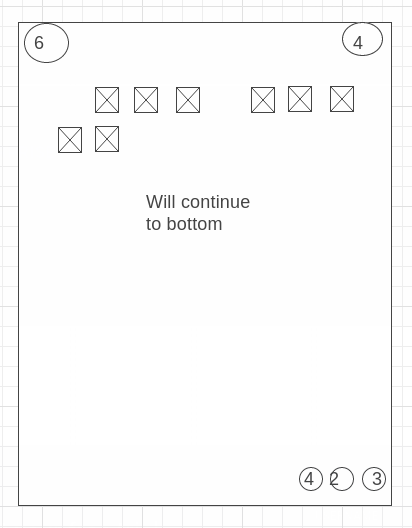
\includegraphics[width=0.7\linewidth]{images/boardWireframe.png}
    \caption{A board wireframe. Slots take up the majority of the board, following the design of the physical game while the marbles are collected in the bottom. This is not the final design as an iterative design process was carried during the implementation to improve ease of use.}
    \label{fig:boardWireframe}
\end{figure}

\subsection{Main Page Design}
The main user interface for the main simulator page was designed after examining other simulators as described in Section \ref{section:background}. Some design decisions to consider from these programs include
\begin{itemize}
    \item The board should be the largest element and in the centre of the page, giving the most clarity and visual weight.
    \item Piece selection should be on the left and include its graphical icon.
    \item Options related to the board could be on the left or right of the board.
    \item Triggering the marbles could be placed under the board. To be similar to the flippers in the physical game.
    \item Speed control could be a slider or a list of set speeds.
\end{itemize}

After examining these simulators three initial wireframes were created for possible page designs. By focusing the design on other implementations it allows users already familiar with these programs to understand this program more easily. The wireframes were created online using draw.io \citep{noauthor_flowchart_nodate}. Different design elements were considered in each with the final wireframe (shown in fig. \ref{fig:wireframe}) being the main design that was improved on during the implementation stage. In this design it was important to have strong emphasis on the board by placing it in the centre of the page. A side navigation bar was chosen to be less intrusive than a top navigation bar and was designed to be hidden or revealed by the user with a button toggle. It was designed that only options available to the user should be shown at any given time and that icons would be greyed out to signify unavailable options to reduce distraction.


\begin{figure}
    \centering
    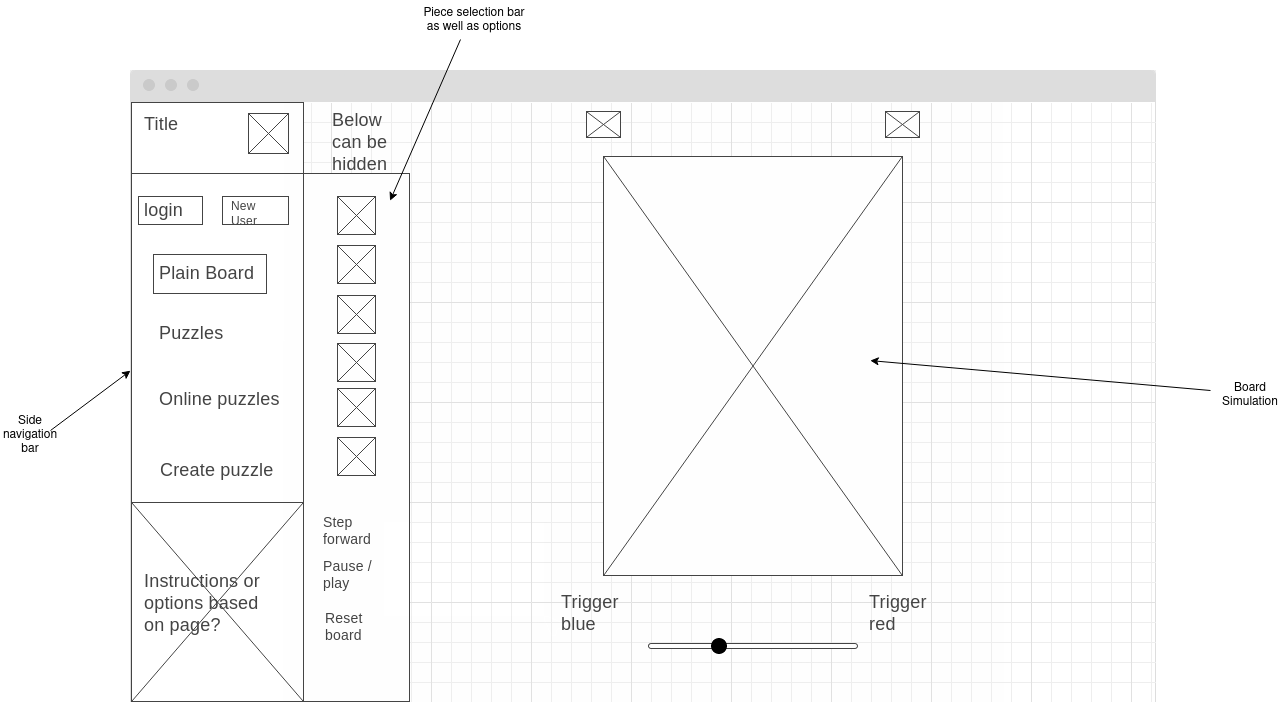
\includegraphics[width=0.8\linewidth]{images/wireframe.png}
    \caption{A wireframe created when designing the main board page. It shows the main position of the board, side selection bar, and side navigation bar with some options. The design was revised during implementation and is shown in the implementation section.}
    \label{fig:wireframe}
\end{figure}

\section{Technologies}
The following technologies were chosen to meet the specification and capture the functional requirements.

\subsection{Angular}
Angular (\cite{noauthor_angular_nodate-1}) was chosen as it is a fully component based Javascript (JS) framework with components split into a model, view, and controller. Typescript (\cite{noauthor_typed_nodate}) is the scripting language used in Angular that compiles down to native JS. It is a superscript of JS with static type checking and allows for greater control over the creation of classes and interfaces. The components in Angular are organised in a hierarchy and can help keep a strong modular design by passing data down to child components only when necessary. Angular comes prepackaged with some useful libraries including a testing framework, routing service, and forms. It is also very easy to add a wide variety of different JS libraries using Node Package Manager (\cite{noauthor_npm_nodate}) allowing more development time spent on implementing the functionality of the program instead of solving issues solved by external libraries.

\subsection{Material UI}
Material UI (\cite{material}) created by Google was chosen as a UI library to add high quality UI elements to the application. Material UI components are highly reliable and already tested to ensure that the UI in the program is easy to use and follows a standard seen in other sites. Material UI components are added to existing code by using a call to an individual component using Angular notation and editing the component using its API.

\subsection{Web Application}
This program was designed as a web application. One reason was the goal to have this program be easily accessible to the target audience so the high portability of a web application was desirable. Second is that the program was designed with user interaction in mind so a web application allows the storing of user data in a backend server that can then be displayed to other users. Lastly a web application is more accessible for users in a classroom environment, as desktop machines may have different hardware specifications across schools and may not allow external software to be installed easily.


%==================================================================================================================================
\chapter{Implementation}
\label{section:implementation}
\section{Angular Framework}
The Angular framework is designed with the model view controller (MVC) pattern as a core principle.  This principle is present in Components, the main building block of an Angular application. 

\subsection{Typescript Classes - Model}
Typescript classes were created to model and contain the domain logic of the application, e.g. 'Board.ts' contains properties and functionality related to a Turing Tumble board. These classes are stored outwith the normal Angular Component file structure and are used to model complex data. A component file, which acts as the controller, can then store and call these models to access and use the models API to update the data.

\subsection{Angular Components}
Angular components are split into a template file, component class file, and an optional style sheet. With each file equivalent to a part in the MVC. A diagram showing this separation is shown here in fig. \ref{fig:angularComp}. 

\textbf{Template file - View}
A component's template file is made up of HTML and Angular template syntax and represents the View. This file will instruct Angular on how to render the component to the screen. This has multiple advantages to base HTML, including the use of template syntax to directly edit the Document Object Model at run time. For example a for loop can repeat a HTML template for every item in a list, e.g. use the same template for all Slots on a board. It also allows child components to be created multiple times with each call creating a new instance of a component with its own separate data. For example multiple calls to a Piece component where each piece has its own data but they are all created from a single definition.

% Template files deals with UI logic and different Angular syntax can updated the view in real time. For example, when displaying a ghost image as shown in \ref{fig:ghostPiece}, a conditional is used to only display the image if the piece can fit in the slot that the user is hoovering over. This makes use of template syntax to allow the same component to update it's view based on user events. 

% Most of the file is written in standard HTML but some important Angular template syntax used in the implementation include
% \begin{itemize}
%     \item \textbf{Angular Directive} - To ensure that templates created by the user are dynamic, angular uses \emph{directives} to transform the template based on the instructions they give. Components are examples of directives as Angular will replace a component selector tag (<app-component>) with the component template at runtime.
%     \item \textbf{<li *ngFor="let item of itemList">} - This is an an example of a \emph{structural Angular directive} which tells angular to repeat the HTML and the children it contains over a list of elements by adding the elements to the DOM multiple times.
%     \item \textbf{<app-example-component>} - This tag links to another user created component, making it a child of the current component. This allows user defined components to be easily mixed in between standard HTML allowing Angular to replace that tag with a call to a component and the template file it contains.
%     \item \textbf{ \{\{componentProperty\}\}} - This \emph{interpolation} syntax allows for data binding between the template file and the component class which contains and can edit the data. If the data were to be updated Angular would refresh the data displayed in the DOM.
%     \item \textbf{[property] = "value"} - This syntax when placed within a HTML or component tag is called \emph{property binding} which can set the data values of child components or set property values in a components API, used extensively for an external component library like material UI. A simple example is <img [src]="imgLink">. The value within the double quotes is a property held within the component class file, named z\emph{imgLink}, this allows the src property of an image tag to be updated dynamically.
%     \item \textbf{<button (click)="clickFunction()">} - The (click) value represents \emph{event binding} in which a DOM event, in this case a button click, can be bound to a response function. In this example a button when clicked by a user will call a \textbf{clickFunction()} held within the component class.
% \end{itemize}

% By allowing data binding in native HTML the responsibility of updating data values and ensuring user inputs are captured correctly is given to Angular and focus can be spent on developing the major functionality of the program without spending development time ensuring JS calls are made correctly. 

\textbf{Component class - Controller}
The component class file, written in Typescript, contains all the logic responsible with connecting the data models and views. These classes are used to contain data and functions to update the models based on user events.  An example would be a component class for a Turing Tumble piece, which contains the Piece object and functions to deal with a user actions, e.g. clicking the piece. They are also responsible with setting the templates state. For example, they contain functionality to edit the state when the component is created or model data changes. The file makes use of external Typescript models and use the models API to react to user events. A useful example of this class is the difficulty filter shown in fig. \ref{fig:puzzleList}. When a user updates the filter, the component class reacts to the user event, decides if the input is valid and then filters the list of puzzles that the template file then displays.

Angular design principles and best practices where used when implementing this program. Following a clear separation of concerns between the various files related to the MVC pattern. Details on best practices were found online (\cite{angular_practices}, \cite{freeman_pro_2017}) and focused on storing domain logic within classes, user event logic within component classes, and UI logic in templates.

\subsection{Angular Services}
A service is a class designed for non-UI functionality that can be inserted into multiple components at run time. For example a service was created that uploads and retrieves data from a backend server. This allowed one service to be created for this functionality that components can use when required. 



\begin{figure}
    \centering
    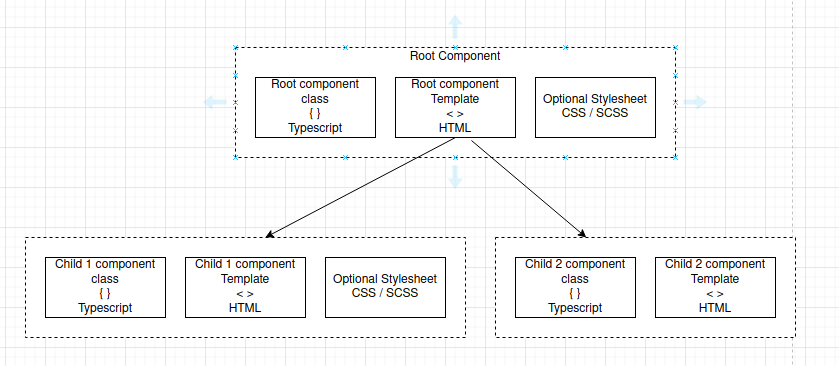
\includegraphics[width=1\linewidth]{images/componentDesign.png}
    \caption{A diagram showing the files included in each Angular component. Including the hierarchy that is created when calling multiple components. Diagram adapted from \cite{noauthor_angular_nodate-2}}
    \label{fig:angularComp}
\end{figure}

% \clearpage

\section{Aesthetics}
\subsection{Material UI}
This library was used to provide a user friendly and visually appealing standard across the program. Various packages were used including buttons, forms, prompt cards, and side navigation bars. This allowed more development time to be spent on functionality and while some development time was still spent arranging the various UI elements, time was saved by including high quality UI building blocks included in this library. It also allowed solutions to common UI problems to be provided by this library, for example the side navigation bar as shown fig. \ref{fig:homePage} was implemented using material UI side-nav component module.

% \subection{Program theme}
% 2 Themes were created, and a change theme button was added on the heading bar to allow users to switch between a 'dark' and 'light' theme as shown in the appendices \ref{fig:themes}, 'dark' theme is used in all other figures. By having 2 distinct themes it allowed users choose the theme they find the most accessible. The themes are stored in a SCSS file contained at the root of the component hierarchy. This theme change is possible due to material UI and applies to all material UI components, leading to a consistency among all UI elements.

\subsection{Piece aesthetics}
The 6 piece icons created for this program were strongly influenced by the design implemented in the physical Turing Tumble, they can be seen in fig. \ref{fig:pieces}. This consistency allows any user familiar with the physical game to be familiar with the pieces and their logic. The colours of the pieces were also influenced by the physical game and each have a distinct colour separate from any other pieces. This attribute and the unique shape of a piece helps improve the individual recognizability. This was found to be no issue in the user evaluation. The pieces icons were created using an online SVG creator \citep{noauthor_method_nodate} and saved as an SVG icon so machines of different resolutions could scale up the icons without losing quality. 

\begin{figure}
    \centering
    \begin{subfigure}[b]{0.20\textwidth}
        
\includegraphics[width=\textwidth]{images/ramp.png}
        \caption{A Ramp piece \\}
        \label{fig:ramp}
    \end{subfigure}
    \begin{subfigure}[b]{0.20\textwidth}
        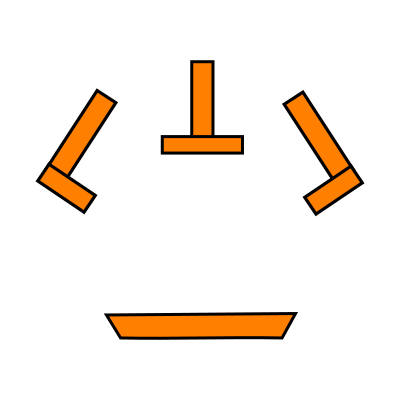
\includegraphics[width=\textwidth]{images/crossover.png}
        \caption{A Crossover piece \\}
        \label{fig:crossover}
    \end{subfigure}
    \begin{subfigure}[b]{0.20\textwidth}
        
\includegraphics[width=\textwidth]{images/bit.png}
        \caption{A Bit piece \\}
        \label{fig:bit}
    \end{subfigure}
    \begin{subfigure}[b]{0.20\textwidth}
        
\includegraphics[width=\textwidth]{images/interceptor.png}
        \caption{An Interceptor piece \\}
        \label{fig:interceptor}
    \end{subfigure}
    \begin{subfigure}[b]{0.20\textwidth}
        \includegraphics[width=\textwidth]{images/Gear.png}
        \caption{A Gear piece \\}
        \label{fig:Gear}
    \end{subfigure}
    \begin{subfigure}[b]{0.20\textwidth}
        \includegraphics[width=\textwidth]{images/Gear-bit.png}
        \caption{A Gear Bit piece \\}
        \label{fig:gearbit}
    \end{subfigure}
    % \begin{subfigure}[b]{0.17\textwidth}
    %     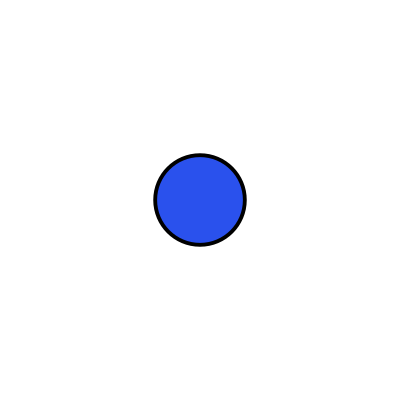
\includegraphics[width=\textwidth]{images/blue-marble.png}
    %     \caption{A blue marble \\}
    %     \label{fig:blueMarble}
    % \end{subfigure}
    % \begin{subfigure}[b]{0.17\textwidth}
    %     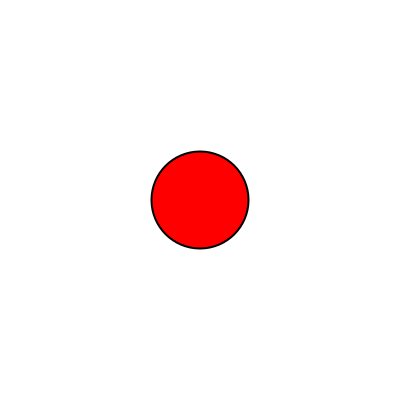
\includegraphics[width=\textwidth]{images/red-marble.png}
    %     \caption{A red marble \\}
    %     \label{fig:redMarble}
    % \end{subfigure}
    \begin{subfigure}[b]{0.20\textwidth}
        
\includegraphics[width=\textwidth]{images/blue-marble-fall.png}
        \caption{A marble falling \\}
        \label{fig:marbleFall}
    \end{subfigure}
    % \begin{subfigure}[b]{0.17\textwidth}
    %     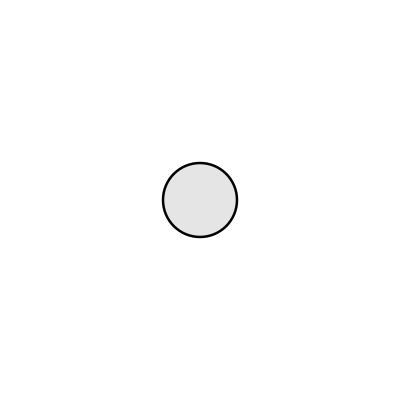
\includegraphics[width=\textwidth]{images/pin.png}
    %     \caption{A Pin}
    %     \label{fig:pin}
    % \end{subfigure}
    % \begin{subfigure}[b]{0.17\textwidth}
    %     
\includegraphics[width=\textwidth]{images/compslot.png}
    %     \caption{A Component Slot \\}
    %     \label{fig:compslot}
    % \end{subfigure}
    \caption{The SVG icons created using \cite{noauthor_method_nodate} for all 6 pieces as well as a marble falling when it reaches no pieces}
    \label{fig:pieces}
\end{figure}

% \subsection{Board aesthetics}
% The aesthetics for the a plain Turing Tumble board as shown in \ref{fig:marbleInPlay} was designed to mimic a physical board as much as possible without adding unnecessary details such as marble dispensers or walls. This minimalist design was chosen to reduce visual clutter and match the design followed by the rest of the program. By having the background a light grey-blue, each piece was designed to contrast with the board background in both themes. The background was also chosen to help give the width and height of the board and ensure that slots didn't appear to 'float'. Two coloured arrows were added at the top of the board to make it easier for users to understand which slot the 2 coloured marbles would enter when first released. The two slot types were chosen to be white to aid contrast with the board background. A blue and red coloured line was added to the bottom of the board to improve understanding of which area are marble would need to be directed towards to trigger the next coloured marble. 


\section{Simulator Features}
This section lists the features implemented to meet the main set of functional requirements concerned with matching the existing Turing Tumble simulators.
% Each feature should start off at the high level and then more information can be added to describe how it was implemented 

\subsection{Board Creation}
Board creation is important to ensure users can create their own (possibly intricate) Turing Tumble boards to simulate and learn with. Users can select the pieces they wish to place from a selection bar at the side of the page. This selection bar contains the list of pieces including its graphic icon as shown on the left in fig. \ref{fig:puzzle}. Once a piece has been selected , a user can then place it in a valid slot. When a user hovers over a slot holding a piece, a 'ghost image' is displayed to give an intuition that a piece can be placed, an example can be seen in fig. \ref{fig:ghostPiece}. This was a suggestion given by multiple users during the evaluation stage to make it clearer where and how pieces can be placed. Users can delete pieces can selecting the delete piece option and selecting the piece they wish to remove.

Unlike other simulators, users don't need to use a different piece for each orientation (e.g. a Bit pointing left or right). Instead if they are holding a reversible piece and click on the same type of piece on the board, it will flip its direction. This was implemented to be more efficient for users to reverse piece direction, this was found to be intuitive in the user evaluations. 

The board and selection bar components were kept separate to improve modularity and single responsibility. When a user clicks a piece on the selection bar this event is captured and sent to the parent component where it then updates the board object. When a user holds a piece, its corresponding icon on the selection bar changes colour to aid understanding of which piece is being held, this is also aided by the ghost image. After clicking a slot on the board, the individual slot will release an event telling its parent board component that it has been clicked, detailing its location. The board will check that a valid slot was clicked before adding this piece to the slot. Within the board component template every slot is created using a separate \emph{Slot component} that is given a unique slot object using an input property which uses Angular data binding to act as parameter for components. This also ensures that when a slot property is updated, the corresponding component updates its view in the DOM, instantly showing this piece to the user in real time.



\begin{figure}
    \centering
    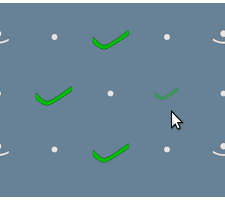
\includegraphics[width=0.4\linewidth]{images/ghostImage.png}
    \caption{A 'ghost image' showing a user where they can place the piece they are holding}
    \label{fig:ghostPiece}
\end{figure}


\subsection{Piece logic}
Each piece available in a physical Turing Tumble board requires its own logical functionality. To allow every piece to be abstracted within the board class, an abstract board piece class was created that contained piece properties. The logic of every piece was created to follow the logic described in the background (Section \ref{section:background}). Each piece would be sent a marble to 'process' and would edit the marbles direction based on its properties and call any internal functions to update its state. By having each piece represented by a class, it allows multiple unique pieces to be created that each have their own state on the board. This is necessary to ensure that pieces placed by users follow the logic found in the physical game such as Bit components each with individual direction.  

% By having each piece extend an abstract class. A single component representing any piece could be created. This component would receive a piece as a parameter and display the necessary graphics to user. By using Angular data binding, this piece would be updated instantly if its state where to change. For example this would ensure that a Bit piece that had processed a marble, displays this in real time before changing the rotation of its graphic. By having real time updates of pieces state, it gives users greater understanding of the boards state at any one time.

\subsection{Gear Bit logic}
% Easier to refer back to logic that is held in the background section
Gear Bits and Gears as follow the logic as described in Section \ref{section:background-pieces}. Users can connect Gear Bits by placing the Gear piece into Pins separating Gear Bits. Once the Gear Bits have been connected the direction of all Gear Bits are updated to be the same, this ensures that the board enforces the rule found within the physical game. When a user clicks on a Gear Bit to change its direction, it will also update any connected Gear Bits. When a marble passes through a Gear Bit, the board will also change the direction of any connected Gear Bits.

To reduce the complexity of a Gear Bits class, the functionality required to simulate this logic was held in the parent board class. When a user places a Gear Bit piece or it processes a marble a function is called to find all neighboring Gear Bits and update their state. This function made use of a breadth first style search where Gears acted liked edges and Gear Bits like vertices. This allowed the Gear Bit pieces to have no knowledge of their sibling pieces and reduce the responsibility its class contained. By pushing this functionality to the parent class, it avoids a complex implementation where each Gear Bit would require the location of any siblings, disrupting the classes abstraction.

\subsection{Marble simulation}
A user must be able to simulate the path a marble would take following the pieces on the board. This is required for a user to understand the effect the configuration of pieces would have on the marble. A button can be clicked to release a red or blue marble. The marble will be released at the top of the board and will then move down having its direction changed by interacting with the pieces. If a a marble reaches a empty slot, a 'falling' icon, shown in fig. \ref{fig:marbleFall}, is displayed to indicate the marble has been reset. This ensures that a user is given feedback to why a marble path was not valid. Each piece has an icon of a marble interacting with the piece, this was created to give the illusion of the marble falling through each piece while ensuring the marbles position is always visible.

A marble has its own state which is updated by each piece it visits. The marble is held by the board object and ensures new marbles are released when it reaches the end of a valid path. Keeping the marble class simple allowed for an easier implementation of marble simulation by leaving the responsibility of updating a marbles position to the board class. 

% Marble validity is achieved by the design of the Turing Tumble board. Pieces can only send marbles to another Component Slot so will always follow a valid set of pieces if present. The walls of a Turing Tumble were implemented by constraining a marbles position if it is sent outside the board width, this allows the fallen marble to appear before it is reset. Ensuring a marbles position is always visible to a user when in execution.

% Two marble dispenser components were created to be displayed above the board. These components had the logic responsible for displaying the amount of marbles available to be released onto the board, it also included 2 buttons to increase or decrease the amount of marbles available. 
In order to reduce the space required by captured marbles which caused issues in other implementations, a collected marbles class was created that only stored the coloured marble sequence collected by a board. This can be seen at the bottom of fig. \ref{fig:marbleInPlay} in which 5 collected marbles are only represented by 3 icons to reduce visual clutter displayed to the user.

\begin{figure}
    \centering
    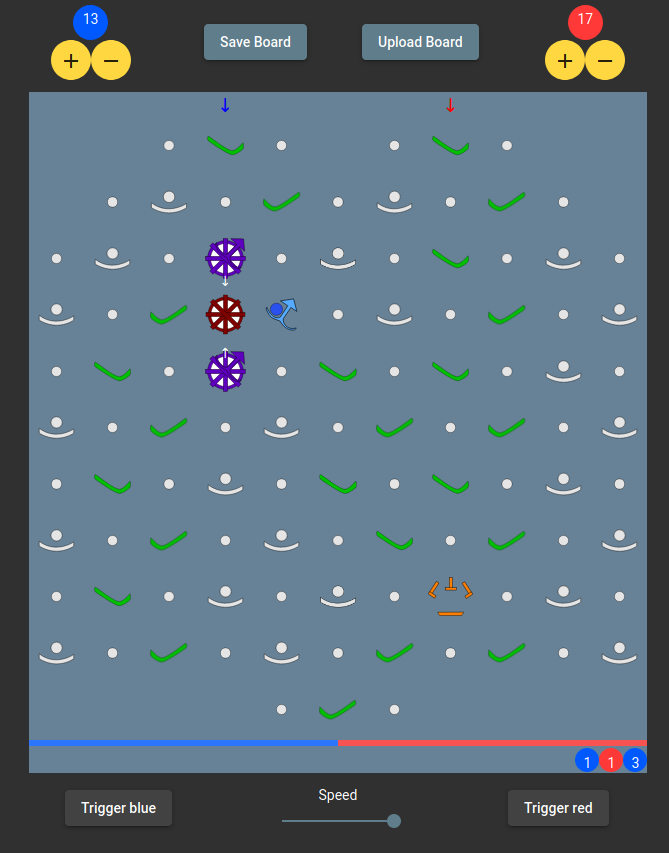
\includegraphics[width=0.5\linewidth]{images/marbleInPlay.png}
    \caption{A view of the board while a marble is currently in play and is displayed to the user. Collected marbles can also be seen at the bottom section of the board}
    \label{fig:marbleInPlay}
\end{figure}

\subsection{Playback features}
An important requirement of the program was to provide execution control. A function was created to implement a single iteration of the marble travelling down the board. Playback functions were then implemented that dealt with calling this function in different sleep intervals to mimic the physical time required by a marble to travel. A pause / play feature was added to allow users to pause execution when required. A speed slider was added below the board to allow users to change the amount of time the execution loop would wait. A slider was added for more accurate execution control compared to a list of presets as found in other simulators. A step forward function was implemented that allows user to click a button to pause the current execution and jump to the next location without waiting. 

\subsection{Board options}
4 separate options were added to aid user control over the board. A user can reset the board removing all pieces, collected marbles, and the in play marble. This gives the user a quick reset function without requiring excessive time spent deleting the individual pieces. A similar reset marbles option was also added to allow users to remove the in play marble and collected marbles, useful to slightly edit the board configuration while resetting the output.

4 example boards were taken from the Turing Tumble site (\cite{turing_tumble_site}), with inspiration from JSTumble (\cite{jstumble}). These examples can be accessed by a button press on the plain board page. It will add the selected piece layout to the board and allows the user to work through more complicated examples of Turing Tumble. This was added to improve users awareness of the computational capabilities of Turing Tumble without requiring them to create the configurations from scratch. 

\subsection{Save and upload configurations}
\label{section:save-upload}
A save and upload board feature was implemented following the design discussed in Section \ref{section:design}. Functions were created to convert an array of slots into a string and vice versa. The implementation allows for an efficient way to represent and store a boards patten that users can then easily understand and edit. The functionality is stored in an external class so it can be used by both components and services requiring the convert functions.

\section{Puzzle Features}
The most important features implemented in this program was the addition of puzzles. Allowing users to play through the set of default Turing Tumble puzzles found in the educator guide (\cite{educator_resources}), gives users a fun external motivator to use the simulator. Puzzle creation was also implemented to allow for the creation of a puzzle environment in which users can create new puzzles for others to play.

\subsection{Puzzle List}
A user can find puzzles in two pages. 'Original Puzzles' which will list the puzzles provided in the Turing Tumble educator guide, and 'Online Puzzles' which will list the puzzles created by other users of the site.

For each page, a list of puzzle card components is displayed on the screen. The list of puzzles has been limited to 10 cards per page, with a paginator added to the bottom. Each puzzle card component as shown in fig. \ref{fig:puzzleList} lists the 6 descriptive properties as described in Section \ref{section:puzzle-background} used to describe the puzzle.  
% \begin{itemize}
%     \item Title - The name given to the puzzle
%     \item Description - The description of a puzzle contains a one or two line summary as to the purpose of the puzzle and what a user should expect to achieve or learn.
%     \item Difficulty Rating - The difficulty rating of a puzzle is used to categorize the puzzles into 5 distinct groups based on a 5 star difficulty scale.
%     \item Starting Set up - The starting set up attribute displays a board with the starting pieces which cannot be replaced or deleted by the user. These pieces constrain the puzzle and the way the user must meet the expected output.
%     \item List of Pieces available - The challenge of Turing Tumble puzzles come with the restriction of pieces available to reach the expected output of the puzzle. This restriction ensures users follow a set pattern of computation to meet the expected output and can create a variety of different challenging puzzles even if they share the same expected output.
%     \item Expected output - This lists the collected marble output that the board should receive to complete the puzzle.
% \end{itemize}

A difficulty filter has been implemented allowing users to filter the list of puzzles by a set of difficulties. This gives the users greater control as to which puzzles they wish to view without having to go through multiple pages of puzzles that may not interest them. This filter was also implemented to help organise the list of user created puzzles. The filter updates the list instantly and doesn't require the page to be reloaded when a new set of difficulties is selected, this adds to usability and avoids unnecessary load times for users.


% \textbf{MAYBE ADD TO DESIGN SECTION INSTEAD?}
% The list using a material UI expansion panel to only show the title and difficulty of a puzzle until a user clicks the puzzle bar. Upon clicking, the user is given a set of tabs they can use to view more information about the puzzle, including its starting set up and list of pieces available. This expanded view also gives the user a button to launch the puzzle. This ensures the list is clean and compact until the user clicks a puzzle they are interested in.  

\begin{figure}
    \centering
    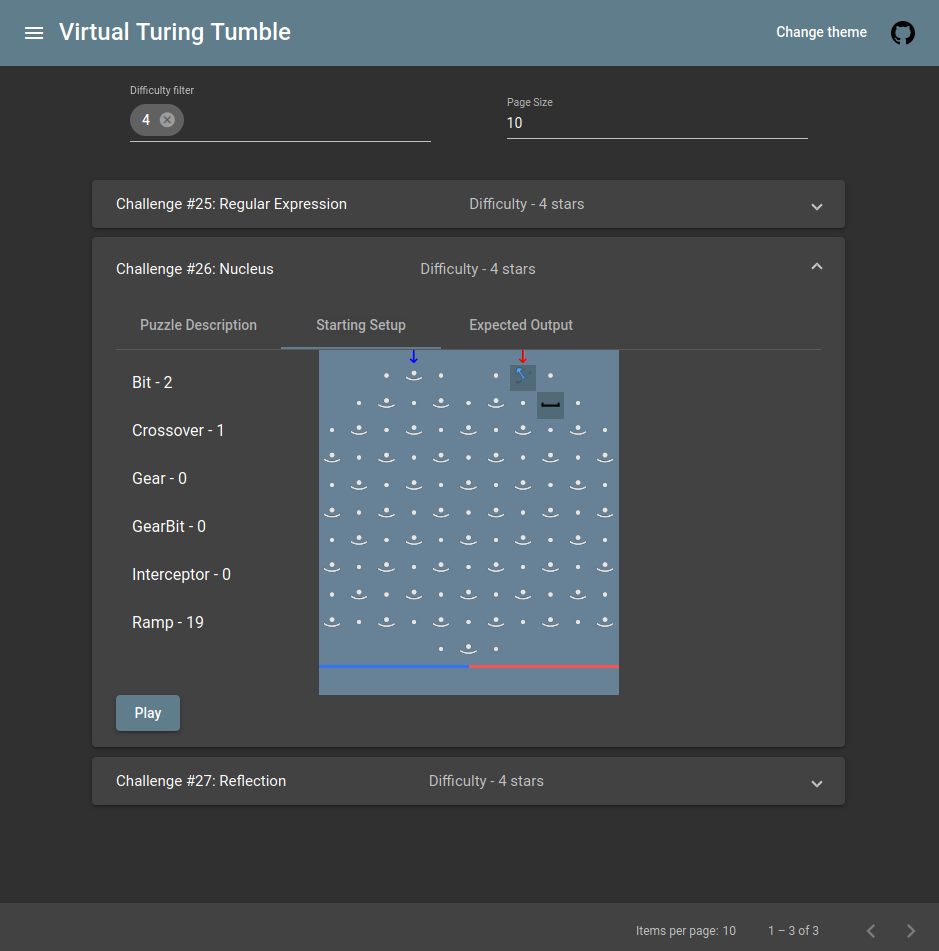
\includegraphics[width=0.65\linewidth]{images/puzzleList.png}
    \caption{A view of the puzzle list used in both the original puzzles and online puzzle pages. One puzzle card has been expanded after clicking, displaying more information about the puzzle}
    \label{fig:puzzleList}
\end{figure}

\subsection{Playing a Puzzle}
A user is presented a board view which uses the same component found in other parts of the program. The user is also given a puzzle title and description above to ensure the user understands the puzzles objective. An example of playing a puzzle is shown in fig. \ref{fig:puzzle}.

A puzzle limits the number of pieces available to a user. This is given by a number next to the pieces icon on the selection bar component. This number is updated dynamically when user places and deletes pieces. The button to select a piece is disabled when the user has no pieces to place. This ensures users understand the number of pieces available to them to complete the puzzle. 

The pieces contained within a puzzles starting setup are highlighted with a darker background. These pieces are 'locked' meaning users can't edit them. This background highlight helps distinguish the starting setup from the slots that users can place pieces. 

% The normal marble buttons used to increase the number of marbles available have been removed as the number of marbles available to complete the puzzle are set as part of the challenge. This ensures the users understand the options aren't available.

A next puzzle button has been added above the selection bar as suggested by a user during evaluations. This will start the next puzzle by updating the data in the component without requiring a reload from the user. The next puzzle is taken from the list that has been filtered by the user, ensuring they only play the next puzzle they are interested in.

\begin{figure}
    \centering
    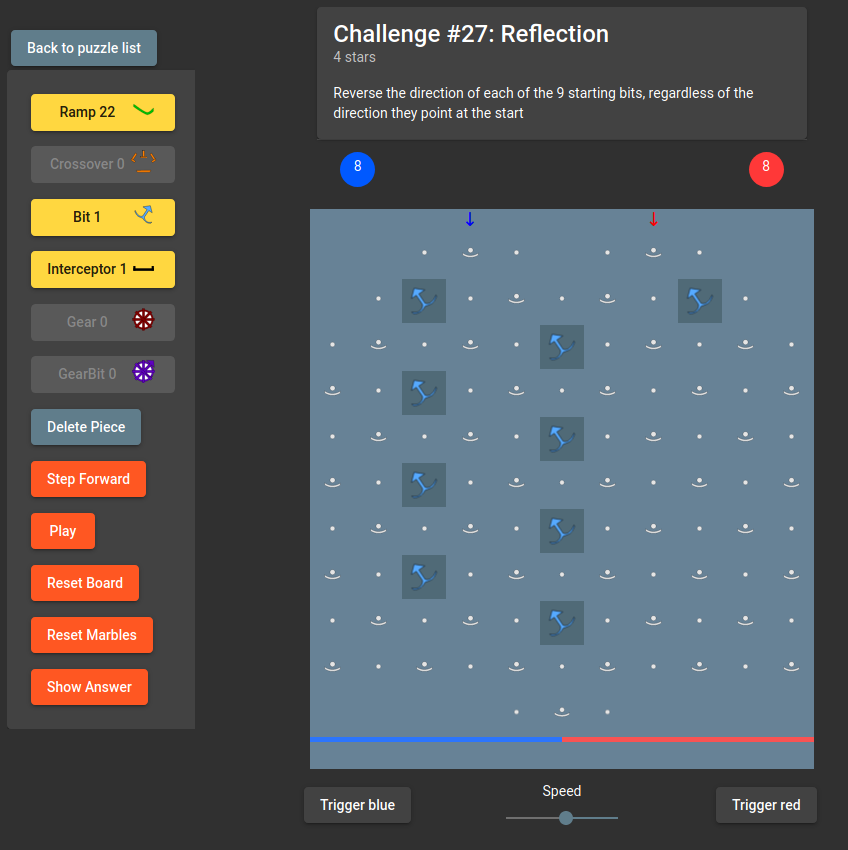
\includegraphics[width=0.65\linewidth]{images/puzzle.png}
    \caption{The view displayed when playing through a puzzle, including the number of pieces available to a user in the selection bar}
    \label{fig:puzzle}
\end{figure}

\subsection{Puzzle Board Class}
\label{section:puzzle-board-class}
To implement and store details of puzzles, a new Puzzle Board class was created which extends the existing board class. This extension allowed all functionality used in simulating, placing, and deleting pieces to be reused when playing a puzzle. By reusing the functionality found in other sections of the site, code duplication is avoided and the user can use the knowledge gained by using the plain board to play through a puzzle. Major extensions of functionality include the puzzle board using the board class' piece placement functionality and checking if a slot had been changed by this function. It then uses this to determine if the piece placement was successful, then updating any piece constraints required by the puzzle. By reusing this functionality, any changes to how users could place pieces will automatically be available for puzzles as well. This was useful for the possibility of future work, if a drag and drop feature were to be implemented. 

The Puzzle Board class also contains new properties to represent parts of a puzzle. Including a \emph{starting slots} property to contain the starting setup of a puzzle, and a \emph{solution slots} property for the puzzle solution.
% Another important piece of functionality that had to be replaced was the reset board option. In the puzzle implementation it was required that resetting the board didn't break the piece amount constraints so the amount of pieces available to the user had to correctly reset.  

\textbf{Puzzle validity}
It was important to ensure any user playing the puzzle couldn't complete it by cheating. While the completion of a puzzle is only for self satisfaction, future work could add leaderboards or user statistics detailing the number of puzzles users complete. This requires a set of functions that ensure puzzles can't be completed by cheating. 

This was met by not allowing extra marbles to be added or removed by the user, so a single execution of the board would be the only way to reach the expected output. A user can only reset the available marbles by using the reset marbles function which also removes the marbles collected by the board. This ensures users can't send down one marble correctly, reset the marbles, and send down the next correct coloured marble.

The amount of pieces users have to complete the puzzle is enforced and checked before a piece can be placed, this ensures no puzzles can be completed outwith the puzzle constraints. 

% \subsection{Puzzle Component}
% The puzzle playing component reuses components already created for other parts of the site. This ensures internal consistency between the different sections of the app. For example the selection bar component is used in multiple pages that allows placement of pieces on the board is present here with different parameters given to this component as part of its created API. This allows the selection bar to update the options and piece information it displays while keeping the same structure and view between two separate pages. 

% The puzzle playing component also makes use of a prompt card component which uses data interpolation to display the different puzzle attributes in the same format for any puzzle that is played. This abstraction is handled by Angular and allows heavy reuse of this component.

\subsection{Creating puzzles}
A puzzle creation system was implemented to meet one of the major goals of the project. This was implemented using a phase system where underlying functions would have different logic depending on the phase a user was in. 

Puzzle creation was implemented using the existing board functionality. This allowed for efficient code reuse but also ensured that the users would already be familiar with how to place and create a configuration on a board so reduced the barrier of entry for a user to create puzzles.

An authentication system was added where users could login to the site either anonymously or using Google login. This would allow created puzzles to display the authors name. This feature was added when a user page was still a main requirement but due to time constraints this was reduced in importance. However authentication is present to ease implementation of any future work requiring it.

\textbf{First phase}
The first phase is the starting set up. This asks the user to place the pieces that will act as the puzzles starting setup. Users only have the option to place the pieces needed for a starting set up, and other unavailable options have been hidden to ensure the user isn't given distracting visual clutter. The user is given details of what is expected of them in a prompt component at the top of the board. After making the starting setup, a button can be clicked to move to the next phase. 

\textbf{Second phase}
Once the puzzles starting setup has been confirmed the user is asked to places the pieces required to solve the puzzle. When placing pieces, the selection bar will take note of how many pieces have been placed. This will store the available pieces a user will have when they play this puzzle. Once the solution has been placed a user then adds the marbles needed and then plays the board using the triggers. Once the collected marbles match the target puzzles result the user clicks a button to confirm the required output of the puzzle. The second phase is shown in fig. \ref{fig:puzzleCreation}. At any time a user can return to the previous set up if they made an error. This was a suggestion given by a user during evaluations to improve the puzzle creation process.


\begin{figure}
    \centering
    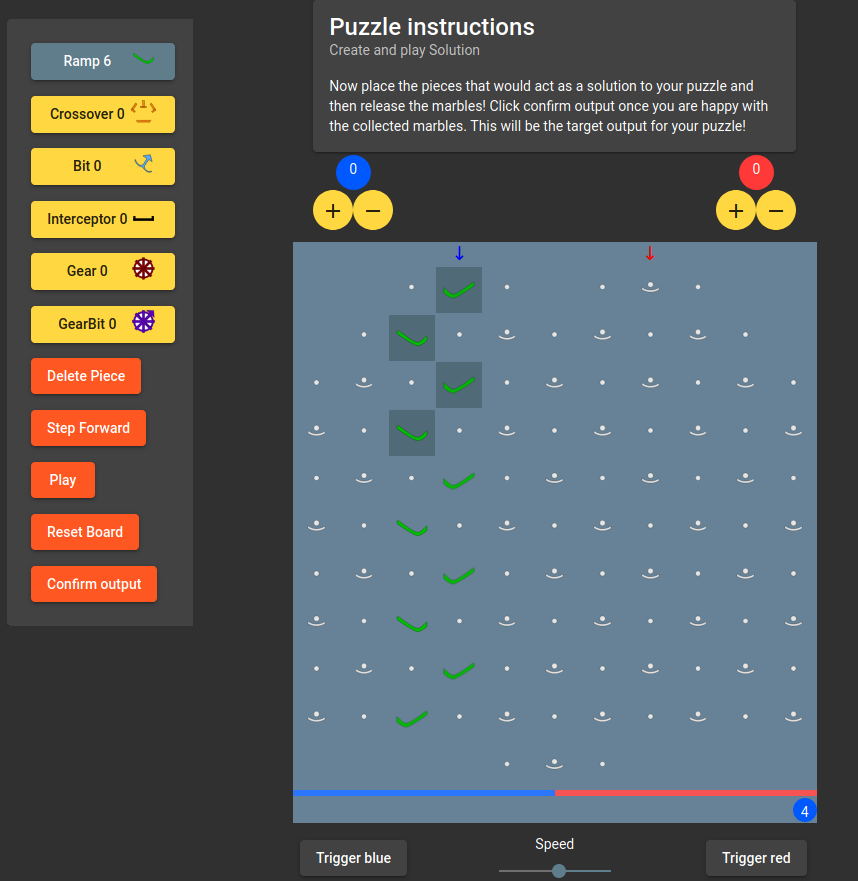
\includegraphics[width=0.65\linewidth]{images/puzzleCreation.png}
    \caption{The second phase of puzzle creation where users must adding the pieces needed to create a solution to the puzzle}
    \label{fig:puzzleCreation}
\end{figure}

\textbf{Final phase}
The final phase gives the user a simple Material UI form to input the title, description, and difficulty for this puzzle. After ensuring the values are valid the puzzle is then submitted by a user click.

\subsection{Puzzle Creation Functionality}
The Puzzle Board class (described in Section \ref{section:puzzle-board-class}) that is used to play puzzles is made during this puzzle creation process. It has functionality extended from the Board class and holds a property related to the phase a user is in. Depending on the phase, different functions will store values related to the puzzle, including the starting setup of the board and the number of pieces required for a solution. After confirming the puzzle in the third phase the descriptive attributes are stored in a \emph{Puzzle Object} which stores these attributes plus a Puzzle Board object that represents the puzzle. An external service is then used to upload the puzzle to the backend Firebase (\cite{firebase}) server.

\textbf{Puzzle Creation Validity}
To ensure a user creates a puzzle which can be solved by an another user. Validity was implemented based on the design described in Section \ref{section:design}.

To ensure a valid starting setup, when a user creates the setup in phase one and moves to the next phase. The slots held by the board are saved and stored in the puzzle boards \emph{starting slots} property which can then be retrieved when someone plays this puzzle. 

The available pieces of a puzzle is not set using an input form. It is calculated during the second phase where a creator places the pieces required for a working solution. This ensures the puzzle creator can not incorrectly set the amount of available pieces such that a player couldn't correctly solve the puzzle. 

The amount of marbles available to a player is calculated by updating the puzzle board object whenever the creator increases or decreases the amount of marbles they use in the second phase. This ensures that a puzzle creator can not set an incorrect amount of marbles such that it would be impossible to complete the puzzle. 

A puzzle creator, can only set the puzzles required output by making a solution to the puzzle and playing through it. This ensures that the puzzle created is feasible and can be completed by at least one user, the creator. This was implemented instead of a possible creation form where users could could create puzzles that were either impossible or harder than the creator could solve.

By implementing built in validity through the creation phase, any puzzles uploaded to the backend server are by design valid and solvable. This is important for future work where more emphasis can be placed on nurturing a puzzle environment for a large number of users. It also adds to user enjoyment by ensuring that a user couldn't play a broken puzzle in the online puzzle list.

% \textbf{Puzzle Creation Component}
% The puzzle creation page makes use of the selection bar, board component, and a information card. The selection bar is given input for the puzzle that is being created and as the current creation phase changes with the user creating the puzzle. The selection bar updates which options it will show or hide to the user. The board component works identically to other parts of the site, but ensures that the users starting set up pieces update to the their locked state once confirmed. A information card component is added to the top of the page to give the user more information on the stages of the puzzle information. This was to give easier instructions to a creator without requiring them to reread the tutorial. 

% The final phase puzzle creation uses a simple material UI form view. Giving the user text fields for text and description, as well as a 5 point ratio box list to enforce difficulty is constrained without the range. The form fields are stored in the external service and enforce all fields are filled before submission.
\section{Backend Service}
A service was created containing the relevant functionality to upload and download data from the backend Firebase server. The Firebase server was easy to use and required simple API calls to interact with. This approach was taken to minimize time needed to be spent on a backend implementation, focusing instead on the puzzle features. 

% This service is injected into the different components. The puzzle creation component uses this service to set and then upload the puzzle created by the user. The puzzle list component, used by both the default puzzles and online puzzles, uses this service to download the specific list of puzzles stored. By injecting this service in multiple components, functionality is reused when required, instead of explicitly rewriting this functionality within components requiring it.

When uploading a puzzle, the details of a puzzle are converted into a smaller more data efficient object. The starting and solution slot properties of the puzzle board are converted into their string representations using the converter functions discussed in Section \ref{section:save-upload}. The puzzle is then converted into JSON and uploaded as a string. This allowed for a simple upload of the puzzle details to the server while maintaining a small file size. It was important to optimise the size of the puzzle to ensure that download times for users remain small. 

% The form used to add puzzle details is also stored within the service. It ensures that all entered by the user is required and a difficulty validator was created to ensure no values outwith the range could be entered.

\section{Usability}
A key goal of the program was to ensure strong ease of use for all users but especially those unfamiliar with Turing Tumble. 

\subsection{Home page}
A home page was created to give users an access point to enter the program that gives details about the simulator, a section detailing the tutorial page, and a brief description about Turing Tumble with a link to its website. It was important that users had a clear understanding of what the program was about as well as giving them direction to the tutorial page. The section on Turing Tumble is designed to get users interested the game, providing motivation to use the site. The home page also includes four boards at the bottom representing the example configurations users can open in the main board page. This gives users some examples of how the board is represented on this program and shows them more complicated configurations to capture interest. The home page can be seen in fig. \ref{fig:homePage}.

\begin{figure}
    \centering
    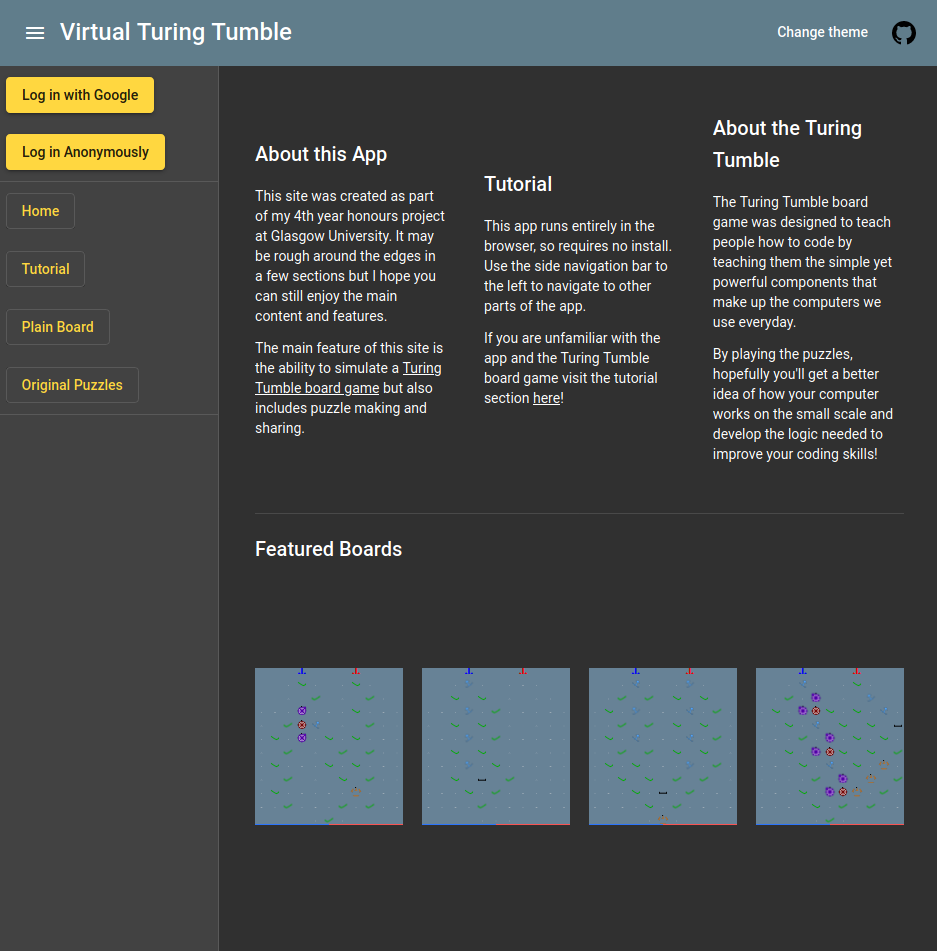
\includegraphics[width=0.65\linewidth]{images/darkTheme.png}
    \caption{A view of the home page of the program, with three paragraphs detailing what the site is about, the tutorial page, and what Turing Tumble is.}
    \label{fig:homePage}
\end{figure}

\subsection{Tutorial}
A tutorial page was created to give users information on different parts of the program. Three sections were created detailing the following information.
\begin{itemize}
    \item It lists information about each page in the program and how to reach these pages using the side navigation bar.
    \item It gives a brief description into the concepts and gameplay of a Turing Tumble and how it is represented in the program.
    \item It contains a description of the options available while simulating a board.
    \item It contains a table detailing the name, image, description, and what every piece is metaphorically like.
    \item It gives details on how to access, choose, and play a puzzle.
    \item It underlines the three phases needed for a user to create their own puzzle.
\end{itemize}

It was important to include a page with detailed instructional information so users would have an understanding of how Turing Tumble works and how it is simulated in this program. The main target audience of the program are users unfamiliar with Turing Tumble so a description of the game was required to give context to the simulator. Detailed information is available on how each individual piece works to ensure users understand why each piece is useful. This can be seen in fig. \ref{fig:tutorial}

\begin{figure}
    \centering
    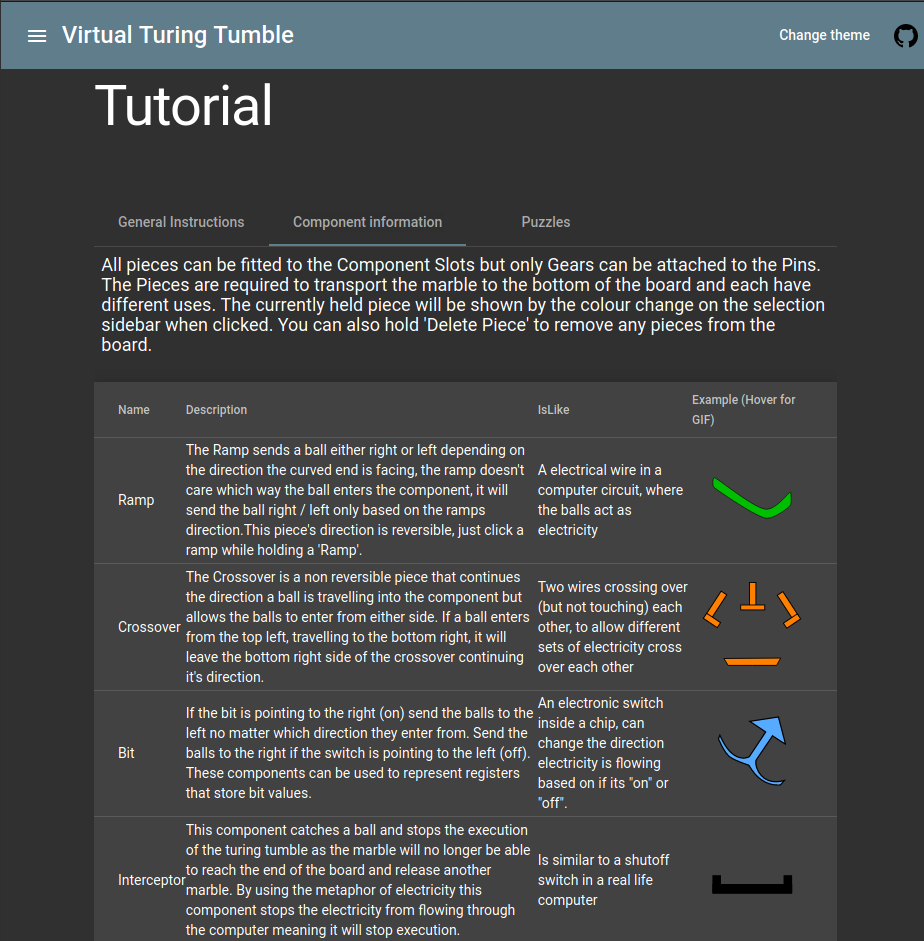
\includegraphics[width=0.65\linewidth]{images/tutorial.png}
    \caption{A view of the tutorial page of the site, including the three separate tabs users can use to access different information sections.}
    \label{fig:tutorial}
\end{figure}


 

\section{Component Benefits}
Angular encourages a modular component approach when developing. This design principle was followed when creating abstract and interactive components. By focusing on creating small compact components, many pages would utilise a set list already used in different sections of the site. As shown by the component diagram (shown in fig. \ref{fig:homeComponent}) for the Home page. The same Board component is created 4 times with each containing a set of slot and piece child components. This allowed all components to follow one source of truth and lead to high reuse of existing code. 

An Input tag can be added to any property in a component class to allow this property to have a value passed to it as parameter. This allowed components to abstract exact details of what data they were displaying to users and allow components to be created for interfaces or abstract classes. One example where this was used was the Piece component. This component has a property where a Board Piece can be passed as a parameter. This allows any of the six pieces to be passed and utilized in this component class. Ensuring that a consistent design and reuse of code was implemented. 

An output property can be added to a component to allow data to be sent 'up' to the parent component by creating an event emitter. The parent component can then capture this event sent by the child component and handle it via functions. This is used in the selection bar component which contains output properties to signify when a button is pressed by the user, the parent component will then capture this event and update the board. This allowed the selection component to not have direct access to the board object and not be given details on the implementation of the options it presents to the user. 

As each created component holds its own independent data, multiple components can be created without data being shared. This is most useful when creating the slots on the board object. Over 106 separate slot components are created to handle the data and any user events for each individual slot. This allowed the functionality for a single slot to be implemented then repeated for every slot on the board.

\begin{figure}
    \centering
    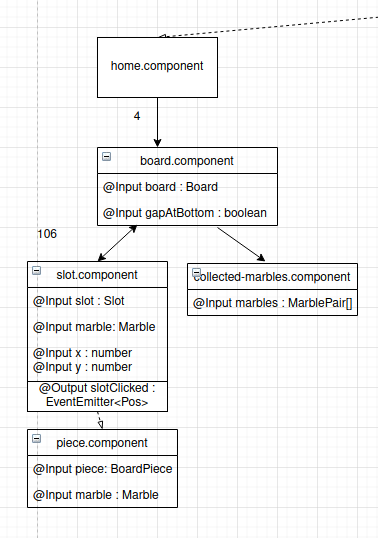
\includegraphics[width=0.45\linewidth]{images/homeComponent.png}
    \caption{A view component hierarchy including the number of child components this page reuses.}
    \label{fig:homeComponent}
\end{figure}

\section{Deployment}
The site was deployed using Github pages (\cite{github_pages}). This allowed easy deployment to a free and always online platform. It was decided that the site would be deployed to ensure that the target audiences of the program can access the program without downloading or installing the necessary files or libraries required to run this program on their own computer. This project can be found at \url{https://lukegall.github.io/Level-4-Solo-Project/home}.

\section{Documentation}
Documentation has been created to provide guidance to other developers on how to install and run this program on their machine. Extensive code documentation was created detailing ever major class and component. This documentation will help other future developers edit and add new features to the program, improving the overall maintainability.

% Maybe cut?
% \section{Issues experienced during implementation}
% \subsection{Passing Router parameters}
% \label{section:issues}
% Routing between different views in Angular is implemented via a 'Router Outlet' component. This component is placed at the root of the web page and then a 'Router Link' can be created between a URL and a component to display. Originally the 'Original Puzzles' and 'Online Puzzles' pages used the same component but depending on the link clicked by the user a puzzle destination was passed as a parameter to obtain the specific list of puzzles. This allowed a link to 'Original Puzzles' to access a generic puzzle list component while passing the path to this list of default created puzzles. The same would have been repeated for Online Puzzles, however when passing this parameter to the router it would display the correct list initially, but if a user was to navigate from 'Original puzzles' to 'Online puzzles' the Router Outlet would not detect a change of component, so would therefore not call the component creation function which pulled the exact data from the Firebase server, leading to no change in view for the user. This was fixed by creating 2 separate components for 'Original Puzzles' and 'Online Puzzles' that had a child component of the abstracted puzzle list component passing the list path using property binding. This allowed an abstract component to be used for both lists of puzzles while ensuring all routing to these components worked as expected.  

% \subsection{Converting data pulled from backend server}

% The program was designed with a focus on an Object Oriented approach, it was decided to have Typescript classes to represent the various objects used in the program, for example a Board and Ramp class. This allowed development to focus on keeping data and methods contained within the objects requiring them. This allowed a separation of concerns between each individual class and reduced the reliance on external services to update board state as originally designed. One issue arose when uploading puzzle data to the firebase server. The data stored in the Firebase server would lose its type information. This caused puzzles downloaded to not correctly execute as the data held had no references to the class methods required to update state. 

% To ensure that data downloaded from the server contained the correct type data, a converter function was created within the external 'make puzzle' service. This converter function would loop through all properties of the data downloaded and assign each property to a new instance of the object required. This fix allowed puzzles uploaded to be downloaded with no data or type loss. Future work can be spent making this function more efficient which would reduce load times for users.

% \subsection{New GearBit when turned}
% The most complex and interesting piece in Turing Tumble is the Gear Bit and the relationship they have with Gears. The original implementation of this feature had the GearBit object calling a function in an external board service which would check if it needed to change its direction by inspecting the state of the board and if the piece was connected to any other Gear Bits. This implementation bypassed the Angular component child relationship and caused warnings to appear and Gear Bits to render incorrectly. This was because a board component would finish rendering to the screen and then a child component would then edit its view bypassing the parent. This goes against Angular best practice so a new implementation had to be designed. Refactoring was undertaking and the functionality required to move sets of Gear Bits was moved to the board object instead of being in the individual GearBit objects. This allowed the view hierarchy to be preserved as the board component contains a board object which would edit its Gear Bit child. This ensured that the child component's data, the Gear Bit, was only edited by the parent so could be rendered in teh correct order by the Angular framework. 

% \subsection{Sets not checking objects}
% For the implementation of GearBit functionality, a breadth first style search function was created to discover the set of all Gear Bits connected via Gear objects. The function required a set of visited Gear and GearBits. An issue was found using the built in Javascript (JS) Set object. The project was written in Typescript, the superset of JS that adds type checking and custom classes. Custom class was created to store the position of each visited Gear or Gear Bit. It was then discovered that the set object in JS doesn't contain type information so any position object added to this set was unique, even if two position objects contained the same x and y property. This lead to issues when clicking a GearBit as it wouldn't exit the loop trying to find all connected pieces, as the base case would never be met, so would search infinitely.  To fix this issue a built in library was used to convert this position object into a string JSON representation, this could then be stored in the set as expected for the breadth first algorithm. 


%==================================================================================================================================
\chapter{Evaluation}
\label{section:evaluation}
Evaluation was carried to out to analyse how well the program meets the functional and non-functional requirements discussed in Section \ref{section:reqs}. Various improvements and suggestions for new features were found with some being added as described in the implementation Section \ref{section:implementation} while others have been added as future work. 

\section{Unit Testing}
% Either talk about the diagram or don't
Unit tests were created to ensure that underlying code met the functional requirements including correctly simulating the logic of Turing Tumble. These tests also ensured refactoring had a safety net to ensure that no internal functionality was accidentally changed. Tests were made using the Jasmine testing framework (\cite{jasmine}). 

% The diagram shows the statistics of the testing coverage provided by the unit tests. Classes were given the most comprehensive tests as they focused more on the underlying logic of the program and included aspects of the program that should never change. For example the logic of the pieces should always match the physical Turing Tumble. The test coverage for components was lower as the tests created did not cover all the elements in the components HTML file. This was seen as acceptable as focus was given to testing the functionality of the program and less on visual elements, that was manually tested or with UI tests. An overall statement coverage of 69\% was achieved showing that most aspects of the program were inspected and tested for correct functionality.

Important features that were tested include:
\begin{itemize}
    \item Ensuring connected Gear Bit pieces will have the same direction and all change when one is clicked.
    \item A user should be able to select a piece from the sidebar and place it in a slot.
    \item A user should be able to delete a piece on the board.
    \item All pieces should have the same logic as the physical Turing Tumble.
    \item A user should be able to turn a board into a text representation and back again without loss of data.
    \item A user should be able to correctly update the number of marbles held by a board.
    \item The program should not allow users to edit the starting set up of a puzzle.
    \item The board should allow a marble to reach the bottom and then trigger the next coloured marble based to the location that it lands.
    % \item Puzzle Boards should lock the starting pieces of a created puzzle when confirmed.
    % \item The amount of marbles in a puzzle should only be increased if in the creation phase.
    \item Puzzles should update the number of pieces available when a user places or deletes pieces.
\end{itemize}

\section{UI Testing}
UI tests were created using the built in end to end testing framework Protractor (\cite{protractor}). This framework would allow certain DOM element's visibility to be tested and could allow simple button presses and router navigation. These tests would launch an instance of the site and travel through various pages by mimicking button presses. These tests ensured that the elements were displayed correctly even when underlying component logic was changed or updated, for example the tutorial page information was still visible after adding a tab system. 

Important UI features tested include:
\begin{itemize}
    \item A welcome message should be displayed to the user on the Home page.
    \item The side navigation bar should be opened and closed when the hamburger icon is clicked.
    \item A user should be able to select a piece on the selection bar to hold it.
    \item The user should be able to navigate to the Tutorial page using the side navigation bar.
    \item The three separate tutorial sub sections should be visible.
    \item The theme of the program should change when a user clicks a button.
    \item A set of puzzles should be viewable when navigating to the Original Puzzles page.
\end{itemize}

\section{Monitored User Tests}
Monitored user tests were carried out to ensure that users could complete the tasks while having the option to ask for help or explanation. The users were encouraged to give suggestions and improvements while working through the tasks. This allowed the user to give feedback on any aspect of the site, including those that were omitted from the evaluation form. These tests also allowed a users approach to be captured, including how they tried to solve a puzzle. 

Five 4th year Computer Science students were chosen for this test, they were expected to find Turing Tumble intuitive so would focus on the websites ease of use instead of the games logic. The meetings were recorded so points made by the users can be recovered at a later date. The task sheet given to the users included four tasks and did not included a lot of explanation on how to complete the tasks, for example they were asked to create a board configuration without instruction on how to use the selection bar. This allowed for analysis to focus on the ease of use a user would have if they were to access the site separately and only have the tutorial. The notes from these meetings can be found in Appendix \ref{section:monitored-eval-notes}.

\subsection{Task Explanation}
\label{taskExplanation}
Users were given an initial set up task followed by 4 tasks, one of which was optional. The full task sheet can be found in the Appendix \ref{section:monitored-tasks}. 

\begin{itemize}
    \item \textbf{Task 0} asked the users the navigate to the tutorial and spend some time reading the page including the basic details of Turing Tumble and the site functionality.
    \item \textbf{Task 1} asked the user to navigate to the plain board, add pieces, and then walk through a basic Ramp configuration. They were then asked to experiment with the Bit and Gear Bit pieces. This allowed users to experience placing pieces and playing Turing Tumble. It also gave an opportunity to give the user an experience with the two of the more complicated pieces and focus on why they are important for the games complexity.
    \item \textbf{Task 2} asked the user open up one of the example boards and observe the addition ability of the board while experimenting with the playback features. This gave the users the opportunity to see one of the more complicated configurations plus experience the playback options.
    \item \textbf{Task 3} asked the user to navigate to the Original Puzzles page, experiment with the difficulty filter, and then to play a puzzle. This allowed users to view the puzzle options on the site and evaluate playing through a puzzle.
    \item \textbf{Task 4} was an optional task that asked users to create their own puzzle using the create puzzle feature. This was given as optional as it could be difficult for people to come up with a puzzle for a game they have just learnt.
\end{itemize}

\subsection{Monitoring Session}
The user was asked to share their screen over a recorded Zoom call. They were told at the start of the meeting what was expected of them, including the ethics brief and how to contact me after the experiment. Notes were taken when a user asked questions or gave any suggestions. The number of times the user needed help was also recorded, for example one user didn't know how to change the direction of a piece. Other notes were taken of issues the user had, for example one user didn't understand which part of the board would release the specific coloured marble.

\subsection{Evaluation Questions}
\label{section:monitored-questions}
The initial question asked if they were familiar with Turing Tumble. Users were then given a variety of questions for each task. These questions were related to the ease of use of different features, with the answer to be given on a numerical five point scale with '5' being 'very positive' and '1' being 'very negative'. These questions are included in the averaged results table (\ref{tab:monitoredResults}). Other questions included how useful puzzles are in learning Turing Tumble, with answers being either 'no', 'somewhat yes' and 'yes'. During the evaluation form, users were also asked for any suggestions that could improve the ease of use of the program. The full question list can be found in Appendix \ref{section:mon-questions}.


\subsection{Results}
Three of the five users surveyed had heard of Turing Tumble before, these users would be expected to find the program more intuitive than their peers as they have an idea of how the game works. The average number of times users asked for help was 2.8. This suggests that overall most users wouldn't require a large amount of outside help to use the program. This is further suggested by the results of the ease of use questions. A table detailing all ease of use questions with the average responses can be found in Table \ref{tab:monitoredResults}.

\begin{table}[]
    \caption{The table of averaged monitored evaluation responses. Only questions with a five point scale were averaged.}\label{tab:monitoredResults}
    \resizebox{\textwidth}{!}{%
    \rowcolors{2}{}{gray!3}
    \begin{tabular}{@{}lll@{}}
        \textbf{Question}                                                                  & \textbf{Average Response} & \textbf{Standard Deviation} \\
        How easy was it to select and place pieces onto the board?                & 4.4              & 0.55               \\
        How easy was it to understand when a marble 'fell' based on the icon?     & 4.4              & 0.55               \\
        How easy was it to change the direction of a piece that was on the board? & 4                & 1.2                \\
        How intuitive was it that two Gear Bits were connected?                   & 2.8              & 0.45               \\
        How easy are the piece icons to uniquely identify?                        & 5                & 0                  \\
        How easy was it to understand the different playback options available?   & 4                & 1                  \\
        How clear was the puzzle list?                                            & 4                & 0.7                \\
        Was the information provided relevant in choosing a puzzle?               & 4.8              & 0.4                \\
        How useful was the difficulty filter?                                     & 4.2              & 1.1                \\
        How clear was it that some pieces couldn't be changed or deleted?         & 4                & 0.7                \\
        How clear was it that you only had a certain number of pieces to complete the puzzle? & 4.8 & 0.4 \\
        How clear was the create starting set up phase?                           & 4.8              & 0.4                \\
        Was it easy to come up with a puzzle by thinking of the solution?         & 4                & 1.2                \\ 
    \end{tabular}%
    }
    \end{table}


\textbf{Task 1}
All users found it easy to select and place pieces onto the board with an average response of 4.4, this suggests that even though drag and drop may initially appear to be more intuitive, the users still found clicking and placing the pieces easy to use. Users had no issues understanding that when a marble had 'fallen' off the board, with an average response of 4.4. This is likely due to the specific marble falling icon displayed. When asked how intuitive it was that two Gear Bits were connected, the average response was 2.8. This is likely as there is no visible UI change when Gear Bits are connected which all users suggested as an improvement and has been added to future work. 
% One user noted that the screen can be visually overwhelming and that a connection between the connected Gear Bits can give a stronger intuition that they influence each other. 

\textbf{Task 2}
When asked how useful this task was in improving understanding of how bits and registers work, four users gave 'Somewhat yes' and one gave 'yes', the users are unsurprisingly familiar with the concepts but the results do help suggest it could have use in teaching. Playback features were overall understood, with an average response of 4, but a couple of the users suggested making them more clear and grouped together with the speed slider. 

\textbf{Task 3}
All users agreed that the puzzle card displayed enough relevant information to help choose a puzzle, with an average response of 4.8. An average response of 4 was given when asked about how clear it was that some pieces were locked, this suggestions that the background colour chance was suitable in conveying the starting setup of a puzzle. 4.8 was the average response when asked how clear it was that a puzzle only had a certain number of pieces to complete the configuration, this suggestions that the number next to the piece icon and locking the button was effective in conveying the piece constraints. All users responded 'Yes' when asked if they think puzzles could be helpful in learning the game. Suggesting that the puzzles were the correct feature to add to this simulator to improve the possible learning capabilities.

\textbf{Task 4}
All users completed this extra task. They all found the starting phase easy to understand, with an average response of 4.8, this was likely due to the specific prompt for each phase of puzzle creation.  

\textbf{Suggestions given during tasks and in evaluation response}
\label{suggestions}
\begin{itemize}
    \item The ability to reset the starting setup when creating a puzzle. This was later implemented as described in Section \ref{section:implementation}.
    \item Add an interactive tutorial to the program.
    \item Let the user choose how many puzzles are displayed per page.
    \item Add a ghost image of a piece when hovering over a slot it can be placed in. Was implemented as described in Section \ref{section:implementation}.
    \item Add a filter to show which direction each piece will send a marble.
    \item Add graphics to show when two or more Gear Bits are connected via Gears.
    \item Add a small clip to explain what each piece does to a marble.
    \item Add a completed filter to the puzzle list to only show puzzles that haven't been attempted.
    \item Allow the puzzles to be filtered by author.
    % \item All the puzzles to be filtered by the type of concept it implements.
\end{itemize}

\textbf{Notes taken while observing users}
\begin{itemize}
    \item One user wasn't sure on the use of the reset marbles button compared to the reset board button. This is likely due to the buttons being very close in functionality, tooltips could be added to give exact definitions.
    \item Multiple users were confused with which marble would be triggered when it reached the bottom. A colour bar was added to help this but it doesn't seem to have helped make it more intuitive. More emphasis in the tutorial could be given to this or add some graphics to show the marble hitting a 'trigger' for another coloured marble.
    \item Some users were unaware of the tooltips for the pieces when hovered over so asked questions based on what each piece does. Could maybe add more information in the tutorial explaining these tooltips or have the currently held piece display its tooltip in a prompt window. This would give the user clear instructions to what the piece does without the possibility of missing the information.
    % \item One user found it difficult to find the different playback options as they didn't assume they would be in the same place as the selection bar. This could be improved by moving the playback options into their own separate component.
    \item A few users didn't initially see that the puzzle page had a paginator at the bottom so assumed that the 5 initial puzzles shown where the only ones available. This can be improved by adding an infinite scroll to get around the paginator.
    % \item A user didn't initially known which side of the speed bar represented faster or slower. This could be made clearer by adding icons to represent an increase and decrease of speed.
    \item Some users tried to complete the puzzle by triggering a blue marble multiple times instead of letting the board spawn the next marbles. This could be improved by only letting the user trigger the marble once unless they reset the marbles or board.
    % \item One user was confused on how to change the direction of a piece and was looking for an option in the selection bar. This can be improved by their suggestion to add a over a piece to indicate it can change direction.
    \item One user made a mistake while creating the starting pieces for their puzzles and tried to go back but was unable. This was later added as a feature.
\end{itemize}

\subsection{Limitations}
While the users were given some time at the start of the study to read the tutorial it was noted by some that it was a lot of information to take in before starting the tasks. This lead to some users not understanding Turing Tumble as they struggled to remember all the rules from the tutorial. This caused some confusion with how various aspects of the game worked which slowed down progress and lead to some questions and suggestions being about the game rather than the program. Some ease of use responses were also low from users that missed explanations in the tutorial or certain tooltips, possibly reducing the accuracy of the average response.

% The main focus of this evaluation was to gain feedback on the ease of use of the program. Ideally the program could be used in multiple school sessions to analyse how useful the puzzles could be for a users motivation and possible learning opportunities. Given the inability to ask pupils to evaluate the site over a long period, only 2 questions were concerned with if the site could be useful for learning to gain a small insight into if future work could explore this further. 

Some users were more willing to ask for help than others. It was unclear if these users were more interested in learning the inner workings of the program rather than if they found the site easy to use. This may have led to the user asking for help when they didn't actually need it. Other users were more reluctant to ask for help even if it seemed like they needed it. For example, two users needed help when they were playing the puzzle incorrectly. It was likely they didn't want to appear to be struggling so were more reluctant to ask for help. Both of these factors may reduce the accuracy of the average number of times users asked for help.


\section{Unmonitored User Evaluations}
% The unmonitored user evaluations were given out after the user returned a sign consent form, which can be found in the appendices. The user was given the ethics brief and was then sent a task sheet giving the details of how to access the site, the task specifications plus a link to the Google form used for the evaluation questions.
Unmonitored user evaluation was carried out to find out how intuitive the program was for users that only had access to the tutorial (i.e. were not supervised). A mix of 4th year Computer Science students and school pupils (aged 16+) studying Computer Science were chosen as both groups are the target audience for this program. This task was seen as a more realistic evaluation of how users would use the site as they would only have the tutorial page to understand the functionality. The task sheet was designed to focus on giving only as much information as required to complete the tasks, with a focus on using the tutorial page, not the task sheet, to learn the program. 

\subsection{Task Specification}
The task specifications for the unmonitored user evaluation follow the tasks given in monitored evaluations (Section \nameref{taskExplanation}), with the only difference being the removal of the section using Gear Bits. This section of the task sheet was deemed too complex and was left in the monitored evaluation as more information could be given as to why the Gear Bits were important and could be used to make the board Turing complete. 

\subsection{Evaluation Questions}
The evaluation questions given were identical to the questions given to the monitored participants (Section \ref{section:monitored-questions}), without the question related to Gear Bits.   

\subsection{Results}
Of the eight responses given, only one user had previously heard of Turing Tumble. This lead to evaluations from users unfamiliar with Turing Tumble, the main target audience. A table detailing all ease of use questions with the average responses can be found in Table \ref{tab:unmonitoredResults}. 

% Please add the following required packages to your document preamble:
% \usepackage{booktabs}
% \usepackage{graphicx}
% \usepackage[normalem]{ulem}
% \useunder{\uline}{\ul}{}
\begin{table}[]
    \caption{The table of averaged unmonitored evaluation results. Only questions asked with a 5 point scale were averaged.}\label{tab:unmonitoredResults}
    \resizebox{\textwidth}{!}{%
    \rowcolors{2}{}{gray!3}
    \begin{tabular}{@{}lll@{}}
    \textbf{Question}                                                                  & \textbf{Average Response} & \textbf{Standard Deviation} \\ 
    How easy was it to select and place pieces onto the board?                & 4.5              & 0.53               \\
    How easy was it to understand when a marble 'fell' based on the icon?     & 3.875            & 1.46               \\
    How easy was it to change the direction of a piece that was on the board? & 4.5              & 0.93               \\
    How easy are the piece icons to uniquely identify?                        & 4.875            & 0.35               \\
    How easy was it to understand the different playback options available?   & 3.75             & 0.88               \\
    How clear was the puzzle list?                                            & 4.5              & 0.75               \\
    Was the information provided relevant in choosing a puzzle?               & 4.5              & 0.75               \\
    How useful was the difficulty filter?                                     & 4.375            & 0.74               \\
    How clear was it that some pieces couldn't be changed or deleted?         & 4                & 1.07               \\
    How clear was it that you only had a certain number of pieces to complete the puzzle? & 4.125 & 1.126 \\
    How clear was the create starting set up phase?                           & 4.2              & 0.83               \\
    Was it easy to come up with a puzzle by thinking of the solution?         & 3                & 1                  \\ 
    \end{tabular}%
    }
    \end{table}

\textbf{Ease of Use Results}
\textbf{Task 1}
The average response when asked how easy it was to understand when a marble 'fell', was 3.875 but with a high standard deviation of 1.46. So while most found it easy to understand, a few users did not. This suggestions that the icon given to the marble falling is suitable for some but not all, possible improvements to this could be deemed as future work. An average response of 4.5 was given when asked about the ease of changing a pieces direction. This suggests that users found it easy to change a pieces direction, but some users didn't find it as easy to understand so a tooltip could maybe be added to help this. When asked if the collected marble component was clear, five users responded 'yes' while three responded 'somewhat clear', this suggests that the collected marble representation is sufficiently intuitive for most users.

\textbf{Task 2}
When asked if the addition example helped improve their knowledge of bits and registers, half of the users responded with 'somewhat helpful', three responded 'yes', with one responding 'no'. This suggests that the simulator could be helpful in teaching some concepts of Computer Science but future work could be carried out to explore this in more depth. All users found it easy to uniquely identify the pieces, with an average response of 4.875, this suggests that they had no issues differentiating the pieces by their individual icons.

\textbf{Task 3 questions}
All users found the information given in the puzzle tabs relevant in choosing a puzzle, with an average response of 4.5. This suggests that the tab system gives enough relevant information to describe a puzzle. Most users found the difficulty filter useful, with an average response of 4.375, but suggestions were given for different filters that have been added as future work. When asked if they think puzzles could help assist in learning Turing Tumble, all users agreed they could, responding with 'Yes'. This suggests that puzzles were the correct feature to add to improve learning within the simulator.

\textbf{Task 4 questions}
Only half of the users chose to complete the final optional task. All users found it clear to create the starting set up, with an average response of 4.2. This suggests that the tutorial and the prompt given to the user was clear enough to understand what part they were creating. The users were split on if it was easy to come up with a puzzle by thinking of the solution, with an average response of 3 but a standard deviation of 1. This suggests that the design requiring a user to come up with a solution to the puzzle may not be the most intuitive when it comes to creation, future work can look to design a possible update to this process.

\textbf{Major unique suggestions given in unmonitored evaluation response}
\begin{itemize}
    \item Add a 'hint' attribute to a puzzle.
    \item Add the ability to create puzzles by using a coding style text input.
    \item Add an animation of the marble dropping out of the board to indicate when it falls.
\end{itemize}

% \emph{Minor suggestions given in unmonitored evaluation response}
% \begin{itemize}
%     \item Make the collected marbles component responsive to the screen size.
% \end{itemize}

Other suggestions were given but were previously covered by the monitored evaluation responses in Section \nameref{suggestions}.

\subsection{Limitations}
% One limitation of the unmonitored survey is that the number of responses given does equate to the number of signed consent forms returned so some users may have looked at the site and decided against the tasks possibly due to initial information overload that the tutorial may not have helped explain. These views would have been useful to gain when evaluating the program.

% The main focus of this evaluation was to gain feedback on the ease of use of the program. Ideally the program could be used in multiple school sessions to analyse how useful the puzzles could be for pupil motivation and learning. Given the inability to ask pupils to evaluate the site over a long period, only 2 questions were concerned with if the site could be useful for learning to gain a small insight into if future work could explore this further. 

Eight responses were gained from this evaluation survey. While valuable information was obtained the number of responses from school pupils was low (2), which is unavoidable given the current pandemic and the inability to go into a school. This feedback would have been insightful as possible future work could be focused on making the program easy to use and fun in a school environment.  

The survey took around 30 minutes to complete yet it still missed some features I would have liked to have tested given more time. I decided to keep the tasks shorter to ensure I didn't lose the attention of the participants. More tasks related to learning via the program would have been desireable but as 50\% of participants didn't complete the last optional task, it can be suggested that any more tasks would have likely reduced user retention and not have gathered useful information.

\section{Issues known about the program}
\label{section:issues}
The current program is not responsive on a mobile device, meaning that if a user was to open it on their phone, various elements would overlap and break. This was known during the design and implementation of the program. To make the program responsive on a mobile device, the front end code focusing on how the elements are displayed would require an external library. This would give different sizes to elements based on the type of device the program is currently displayed on. This was seen as something outwith the scope of the project during the design stage but could be an issue for any user wishing to open the site on their phone.
          % \item The program sends the puzzle data to the backend firebase server by converting the puzzle object to JSON representation then saving this file in the server. This method was chosen to focus on getting the data stored correctly and then spending more development time on the user facing features of puzzle creation and playing. A single default puzzle is 19.8 kB large when stored on the server. A fix to this would be remove the current implementation of sending up the entire puzzle object and instead only send up the details of changes and important data for example instead of sending up the list of slots for the set up and solution slot lists. A single JSON file can be made that details where pieces are located for each set up instead of sending up data about the board that is already known for example the number of Pin and Component Slots stored in a board object. This issue is something that would improve the backend performance for the site and would lead to a more efficient program.

        %   REWRITE
As noted by some users during the monitored evaluation, some aspects of the site are not fully responsive. This means they can reduce some parts of the UI brake when the screen size changes. For example if the user is playing a puzzle and then reduces the width of their browser, the selection bar overlaps the board, meaning they can't place pieces. This issue was known while creating the site but the development time required to fix this was not seen as valuable when compared to other features. As future work, responsive front end code should be added so that the board and selection bar don't overlap on each over, for example the selection bar could get hidden if the width reduces to a certain limit. This would improve ease of use for the user.
          % \item Full animation of the board involving gravity was explored as a possible avenue for implementation. It was decided early on that more focus should be given towards creating a puzzle environment for users rather than spending extra development time on full animation. Full animation is a desired to greatly improve user feedback and help aid understanding of the board while in play. One issue with the current design of the program is a focus on having a collection of small modular components each with its own HTML file. This doesn't lead naturally to the extension of using an external physics library as a lot of code would need to be changed to deal with the api calls and gravity logic. It will still be included in future work but it is important to evaluate the design of the program doesn't lead itself naturally to this new feature.


\section{Program efficiency via lighthouse}
\label{section:efficiency}
In order to evaluate the programs efficiency and performance, Lighthouse (\cite{noauthor_lighthouse_nodate}) was used to generate a report on the performance, accessibly, and best practices used on each page. The report also gave suggestions to why some metrics may be lower plus suggestions to improve them. The overall scores for 4 pages are shown in Table \ref{tab:lighthouse}.  

\begin{table}[]
    \caption{The table of lighthouse metric scores for 4 pages of the program.}\label{tab:lighthouse}
    \rowcolors{2}{}{gray!3}
    \begin{tabular}{llllll}
        \textbf{Page}            & \textbf{Performance} & \textbf{Accessibility} & \textbf{Best Practices} & \textbf{Speed Index} \\
        Home            & 48          & 100           & 93             & 3.7s                            \\
        Plain Board     & 55          & 87            & 93             & 4.1s                            \\
        Tutorial        & 72          & 96            & 93             & 3.5s                            \\
        Default Puzzles & 63          & 98            & 93             & 3.9s                           
    \end{tabular}
\end{table}

As shown in table \ref{tab:lighthouse} the performance was acceptable for most pages but not high enough overall to meet the non-functional requirement related to performance. Future work can set out to improve these performance metrics. More focus was spent on the features available for users rather than diverting development time towards performance metrics. Performance wasn't noted as an issue when users undertook the evaluation so while even though high scores were not met it is deemed suitable for the scope of the project. 

% The Home and Plain Board pages were shown to have the longest Largest Contentful Paint time, this metric describes the time taken to display the largest text or graphic content on the page. Both pages include large amounts of data to display the board with all its icons and Board parts i.e. 4 example boards on the Home page. Other suggestions to improve performance across all pages was to reduce the DOM size, this is down to the high modulation of components that was chosen for the design leading to large list of HTML components on most pages. This wss seen as an acceptable compromise as high component design reduced repeated code during development and allowed for greater abstraction. Future work can be given to explore avenues to improve these performance metrics across all pages taking note of the opportunities identify by lighthouse as well as focusing on minimise component size and cutting down on unnecessary DOM size.   

\section{Overall}
\subsection{Functional Requirement verification}

All 'must have' functional requirements described in Section \ref{section:reqs} were demonstrated to have been met by users in the evaluation tasks. Including users placing and deleting pieces, walking through more complex examples related to addition, and asking users to play through a puzzle. 9 users (70\% of total participants) completed task 4 showing that the 'create puzzle' feature was also met. Unit tests were created to show that the program meets requirements related to Turing Tumble logic.

All 'should have' requirements were met and demonstrated by users in the evaluation tasks and their responses. The only requirement not demonstrated by users involved the saving and uploading of the board configurations, however this feature was manually and unit tested to ensure it worked as expected. 

All but two of the 'could have' requirements were met. The difficulty filter was directly tested by the user task, while multiple users commented on the tooltips over pieces. The change theme feature was tested manually by the program developer so can be seen as having been met. One requirement not met was the ability for users to save complex configurations of pieces for later use, this can be seen as future work. The final requirement not met included an ability for users to comment and rate other puzzles. This can also be seen as future work. 

No 'would be nice to have' requirements were met and have all been noted as future work.

\subsection{Non-functional Requirement verification}
\textbf{No existing knowledge of Turing Tumble} should be required to use the program. 9 out of the 13 users that participated in the user experiments had not previously heard of Turing Tumble. As all users completed the first three tasks only using the tutorial to guide them, this satisfies the given requirement.

\textbf{Should be intuitive}. For all questions related to the ease of use, all but one of the average responses were deemed high enough for this requirement to be met. Only one feature, related to intuitiveness of Gear Bits had a low average and future work could improve this. 

\textbf{Should be runnable}. All users managed to run the program without issue, therefore this requirement has been met.

\textbf{Should be quick and efficient}. As shown by the section on efficiency (Section \ref{section:efficiency}), this hasn't been met. Future work can be to improve efficiency scores for the program. As this was a 'could have' requirement it was not deemed useful to divert development time towards this. 

\textbf{Runnable on Mobile devices}. As discussed in Section \ref{section:issues}, this was not met due to development time but as it was deemed a 'would be nice to have' requirement this is seen as acceptable. 

\section{Program Goals}

\textbf{Simulate a Turing Tumble board}. This goal was met as shown by the tasks users successfully carried out as well as the example boards stored on the site that follow the logic found in the physical game.

\textbf{Users can build their own Turing Tumble configurations}. This was goal was met as shown by the user evaluations in which users build configurations and puzzles.

\textbf{Increase learning via Puzzles}. Puzzles were successfully created and can be played as shown by task 3 of the user evaluations. Users also agreed that puzzles could be used to help teach Turing Tumble.

\textbf{Should be easy to use and understand}. The responses from the evaluations show that users found all aspects easy to understand. With all but one feature evaluated getting an average positive response on ease of use. 

\textbf{Puzzle environment to be created by users}. Task 4 of the user evaluation shows that this goal was implemented with users finding the puzzle creation system easy to use and understand. Users created puzzles as part of the task with more puzzles possible with higher user uptake. 


% Maybe a section comparing to features in other products?



%==================================================================================================================================
\chapter{Conclusion}
\section{Summary}
This project looked at creating software capable of simulating Turing Tumble and adding features to improve the learning possible through the game. The first main focus of the project was to create a faithful simulation of Turing Tumble, with the rules and logic present in the physical game being present within the program, allowing a user to build any complex configuration possible on the physical board within this simulator. This allows the program to be a faithful simulator in which users can learn skills that can be directly applied to a physical version. The program had a focus on ease of use for users unfamiliar with a Turing Tumble board, the addition of a clear tutorial, tooltips, and a clean aesthetic were added to meet this. Examples of complex board set ups were added to convey the computational power of the game to new users. 

It was decided that it was important to focus on features that could aid a user learning with the simulator. Therefore it was decided that adding puzzles would be the main focus of the program after successfully simulating the game. This would add a unique feature to this program while giving users a clear progression path and objectives to aid motivation for playing and learning with Turing Tumble. A puzzle creation feature was also added to allow users to create their own puzzles, creating an environment that can encourage more users to play with the simulator. 

Evaluation was carried out as listed in Section \ref{section:evaluation} that focused on usability on the two main sections of the program, simulation of  Turing Tumble and the puzzle features. All \emph{must have} functional and non-functional requirements were shown to have been met by the program through the use of user evaluations and unit tests. The main program goals were met by user evaluations and manual testing by the program developer. The main two goals of the project were to simulate a Turing Tumble correctly and provide a puzzle environment for users to learn. The main disadvantage of the program was the lack of some features found in other simulators including full gravity simulation and custom board set up, this is the first area covered in the future work section.

\section{Future Work}
\label{section:future-work}
\subsection{Full Animation}
An important non-functional requirement was to make the program easy to understand for users unfamiliar with the game. While the program does contain a form of animation with the marble travelling down the board in steps, time could be spent adding full gravity simulation as similar to other simulators. By adding ful animation, the user experience would be improved as a clearer simulation of the marble travelling down the board could help new users understand the exact logic of the pieces.

\subsection{Fix issues identified}
As stated in Section \ref{section:issues}, some issues are currently known about the program. These issues could be investigated and fixed to improve the overall program experience for the user and lead to a better learning environment. Full animation was previously mentioned, but other issues include the program not being responsive on mobile devices. Ensuring that the site is easy to access in a different environment would allow users to access the site with a device of their choosing.

\subsection{Custom Boards}
A feature available in some other simulators was the addition of allowing users to customise the dimensions and logical elements of the board itself. This includes adding new slots to the board to increase its size or to add new locations of marble dispensers or flippers. As Turing Tumble is designed to be Turing Complete, by allowing larger and more complex boards, users would be able to create more complicated configurations and in turn puzzles. New puzzle categories could then be added to accommodate these new boards, giving a higher difficulty level for users to play with.  

\subsection{Custom Pieces}
Gear Bits can be combined with Gears to produce more complicated logical components. They can be used to create flip flops, set switches, and fixed position switches. New features could be added to allow users to create their own combination of Gear Bits and Gears and save these combinations for later use. This could encourage users to experiment with more complicated piece configurations and better explore the computational power of Turing Tumble.

\subsection{Greater Focus on learning}
One area of future work would be to evaluate the usefulness of this simulator in a classroom environment. Turing Tumble is designed to be used in classrooms so more features could be added to improve this program for classroom use including custom boards as mentioned above or puzzle compilation statistics for pupils. Evaluation could be carried out in classrooms focusing on the programs ease of use for teachers and if the simulator has any possible learning benefits for pupils logic based problem solving skills. 

\subsection{Performance Increase}
As mentioned in Section \ref{section:efficiency}, the performance was deemed as too low to met the non-functional requirement related to performance. The classes modelling the board and puzzles could be refactored to improve data storage to increase program performance for future users. The home page could also be redesigned to reduce the initial high data load a user experiences when accessing the site. A more efficient site would improve the user experience increasing the likelihood of users wanting to use the program again. 

\subsection{User Suggestions}
Various user added suggestions during the evaluations. Time could be spent adding these suggestions to the program to improve the user experience, ease of use, and puzzle environment. Some important suggestions that should be focused on include: 
\begin{itemize}
    \item An interactive tutorial that could reduce the information overload some users experienced with the static tutorial as well as give exact examples on how pieces work.
    \item Add graphics to show when Gear Bits were connected. This addition could improve the least understood feature and improve the ease of use of the most complex and interesting piece within the game.
    \item Various search tools were suggested to narrow down the puzzle list to the users preference, including author search, concept the puzzle tests, pieces used, and if it was completed previously.
    \item Different methods to create puzzles were also suggested including using an input style similar to a programming language.
\end{itemize}


\subsection{Puzzle Ecosystem improvements}
Currently a user can login via a Google account or anonymously. If a user logs in via Google, any puzzle created by them is assigned name and is displayed to other users on the selection page. New features could be added to improve the environment of custom puzzles. Including allowing comments to be placed under puzzles, ratings, or more custom filters. By adding new features to improve the puzzle environment, it could encourage more puzzles to be created and in turn more opportunities for users to learn via Turing Tumble. Quality of life improvements for a logged in user could also be added, including the ability to edit or delete created puzzles as well as a user page to edit user specific site settings.

\section{Reflection}
On reflection, this project was an excellent learning opportunity especially when it came to learning how to design and implement a large scale software product. A clear abstraction found in Angular between a components user facing display and internal data was found to be very helpful in reducing the amount of code repeated across the various pages of the program. Useability of the program was explored during development and user evaluations were incredibly valuable in aiding the design of clear and easy to use interfaces while providing excellent suggestions for improvements that could be added to the project.

If I was to do this project again, more focus would have been spent learning different graphical libraries for displaying the Turing Tumble board. While the current implementation lead to great code reuse and abstraction, it would be difficult to implement full animation due to the reliance of small individual components. HTML canvas (\cite{html_canvas}) could have been used to draw the Turing Tumble board and update pieces when required. This could have allowed a more accurate representation of the board, while possibly increasing performance by reducing the number of components on the screen.

One suggestion I would give any new student embarking on a similar project would be to really spend the first weeks getting very familiar with the language of implementation. While being confident in Angular, more time could have been spent learning more about the framework as many hours were spent dealing with errors and issues caused by my lack of knowledge around the framework. These gaps of knowledge were later filled during implementation however the time spent dealing with these issues could have been spent adding more features. 

%==================================================================================================================================
%
% 
%==================================================================================================================================
%  APPENDICES  

\begin{appendices}

    \chapter{Appendices}

    
    
    % \section{Monitored response tables}
    % The table below lists a summary of ease of use question responses. 
    
    
    % \begin{table}[h]
    %     \resizebox{\textwidth}{!}{%
    %         \begin{tabular}{llllllll}
    %             Question                    & Responses &   &   &   &   & Average & Standard Deviation \\
    %             Place pieces                & 4         & 5 & 5 & 4 & 4 & 4.4     & 0.55               \\
    %             Marble falling              & 4         & 5 & 4 & 5 & 4 & 4.4     & 0.55               \\
    %             Change Direction            & 2         & 4 & 5 & 5 & 4 & 4       & 1.2                \\
    %             Gear Bits connected         & 3         & 3 & 3 & 2 & 3 & 2.8     & 0.45               \\
    %             Identify piece icons        & 5         & 5 & 5 & 5 & 5 & 5       & 0                  \\
    %             Playback options            & 5         & 4 & 3 & 3 & 5 & 4       & 1                  \\
    %             Puzzle list                 & 3         & 5 & 4 & 4 & 4 & 4       & 0.7                \\
    %             Relevant puzzle information & 4         & 5 & 5 & 5 & 5 & 4.8     & 0.4                \\
    %             Difficulty Filter           & 3         & 5 & 3 & 5 & 5 & 4.2     & 1.1                \\
    %             Locked pieces               & 5         & 4 & 4 & 4 & 3 & 4       & 0.7                \\
    %             Restricted number of pieces & 5         & 4 & 5 & 5 & 5 & 4.8     & 0.4                \\
    %             Starting set up phase       & 5         & 5 & 5 & 4 & 5 & 4.8     & 0.4                \\
    %             Ease of puzzle creation     & 2         & 4 & 5 & 4 & 5 & 4       & 1.2               
    %         \end{tabular}%
    %     }
    % \end{table}

%     \newpage
% \section{Unmonitored User Results}
% The table below lists a summary of ease of use question responses. 


% \begin{table}[h]
%     \resizebox{\textwidth}{!}{%
%     \begin{tabular}{lllllllllll}
%     Question                    & Responses &   &   &   &   &   &   &   & Average & Standard Deviation \\
%     Place pieces                & 5         & 4 & 5 & 5 & 4 & 4 & 5 & 4 & 4.5     & 0.53               \\
%     Marble falling              & 5         & 5 & 5 & 1 & 4 & 3 & 3 & 5 & 3.875   & 1.46               \\
%     Change Direction            & 5         & 5 & 3 & 5 & 5 & 5 & 5 & 3 & 4.5     & 0.93               \\
%     Identify piece icons        & 5         & 5 & 5 & 5 & 4 & 4 & 4 & 5 & 4.875   & 0.35               \\
%     Playback options            & 5         & 4 & 2 & 4 & 4 & 4 & 4 & 3 & 3.75    & 0.88               \\
%     Puzzle list                 & 5         & 3 & 5 & 5 & 5 & 4 & 5 & 4 & 4.5     & 0.75               \\
%     Relevant puzzle information & 5         & 5 & 5 & 5 & 4 & 4 & 5 & 3 & 4.5     & 0.75               \\
%     Difficulty Filter           & 4         & 5 & 5 & 5 & 4 & 3 & 5 & 4 & 4.375   & 0.74               \\
%     Locked pieces               & 4         & 5 & 5 & 2 & 5 & 3 & 4 & 4 & 4       & 1.07               \\
%     Restricted number of pieces & 5         & 4 & 4 & 5 & 5 & 3 & 5 & 2 & 4.125   & 1.126              \\
%     Starting set up phase       & 5         & 4 & 4 &   & 3 &   &   & 5 & 4.2     & 0.83               \\
%     Ease of puzzle creation     & 2         & 2 & 4 &   & 4 &   &   & 3 & 3       & 1                 
%     \end{tabular}%
%     }
%     \end{table}
%     \newpage

% \section{Unmonitored Consent Form}
% This was form was sent out to possible users. Once signed and returned they were sent the task sheet.

% 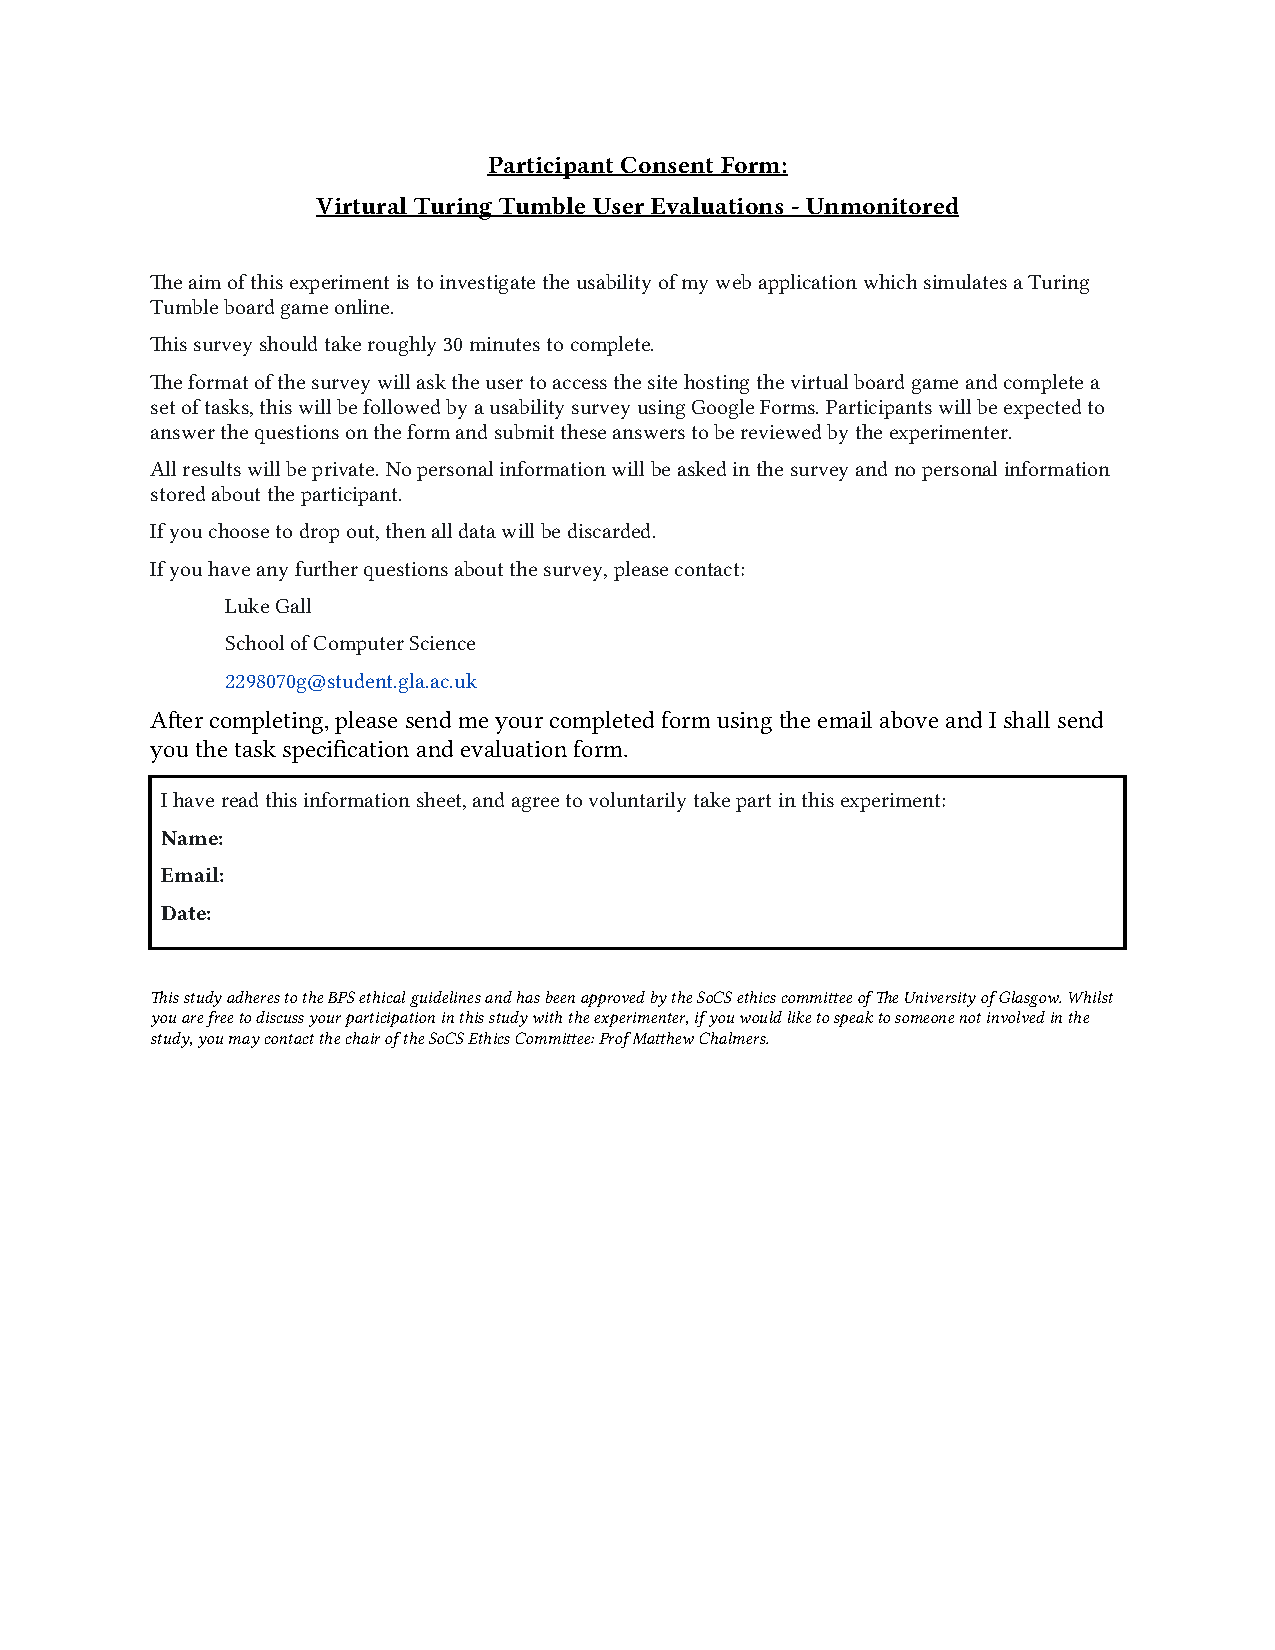
\includepdf{images/unmonitoredConsent.pdf}
% \section{Unmonitored Task Sheet}
% \label{section:unmon-task-sheet}
% 
\includepdf[pages=-]{images/taskSpecUnmonitored.pdf}
% \section{Unmonitored Evaluation Questions}
% 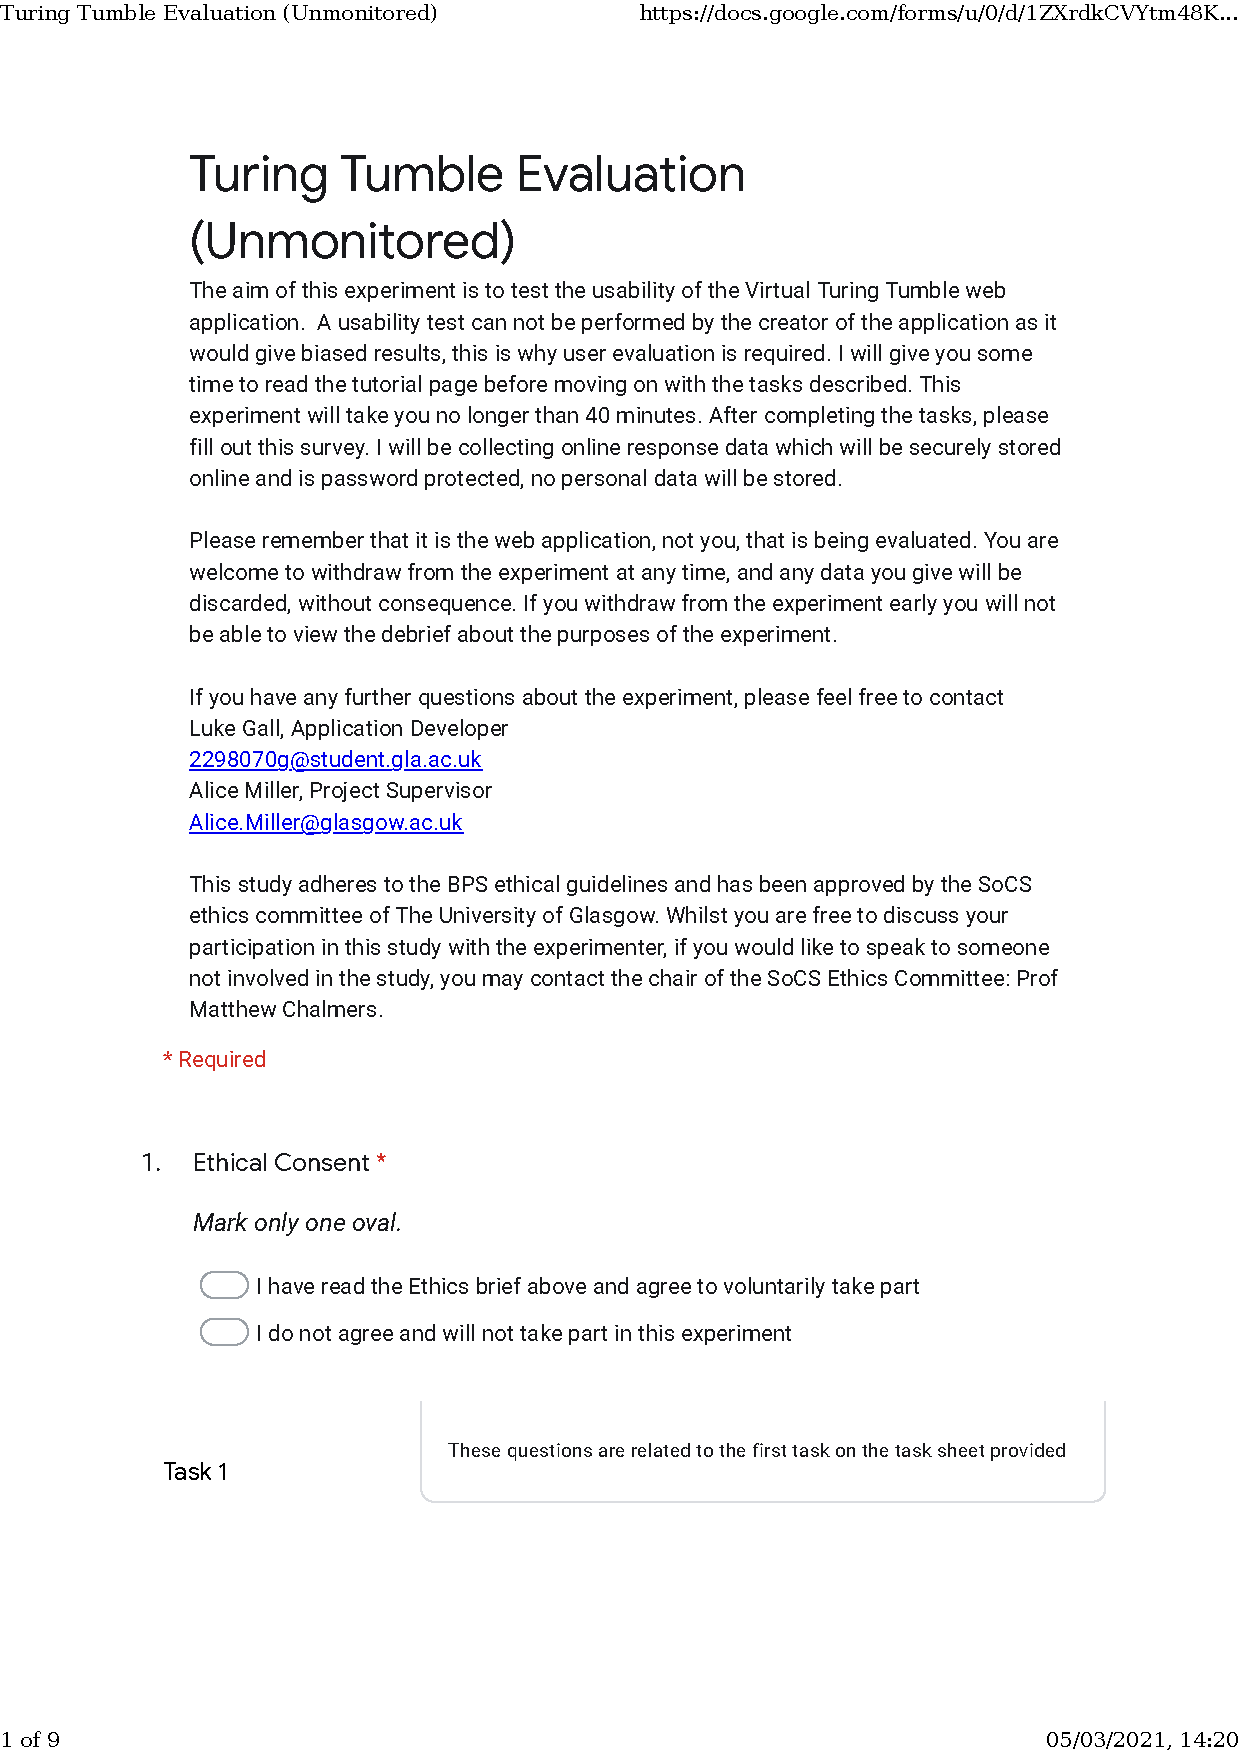
\includepdf[pages=-]{images/unmonitoredQuestions.pdf}
% \section{Unmonitored Evaluation Responses}
% 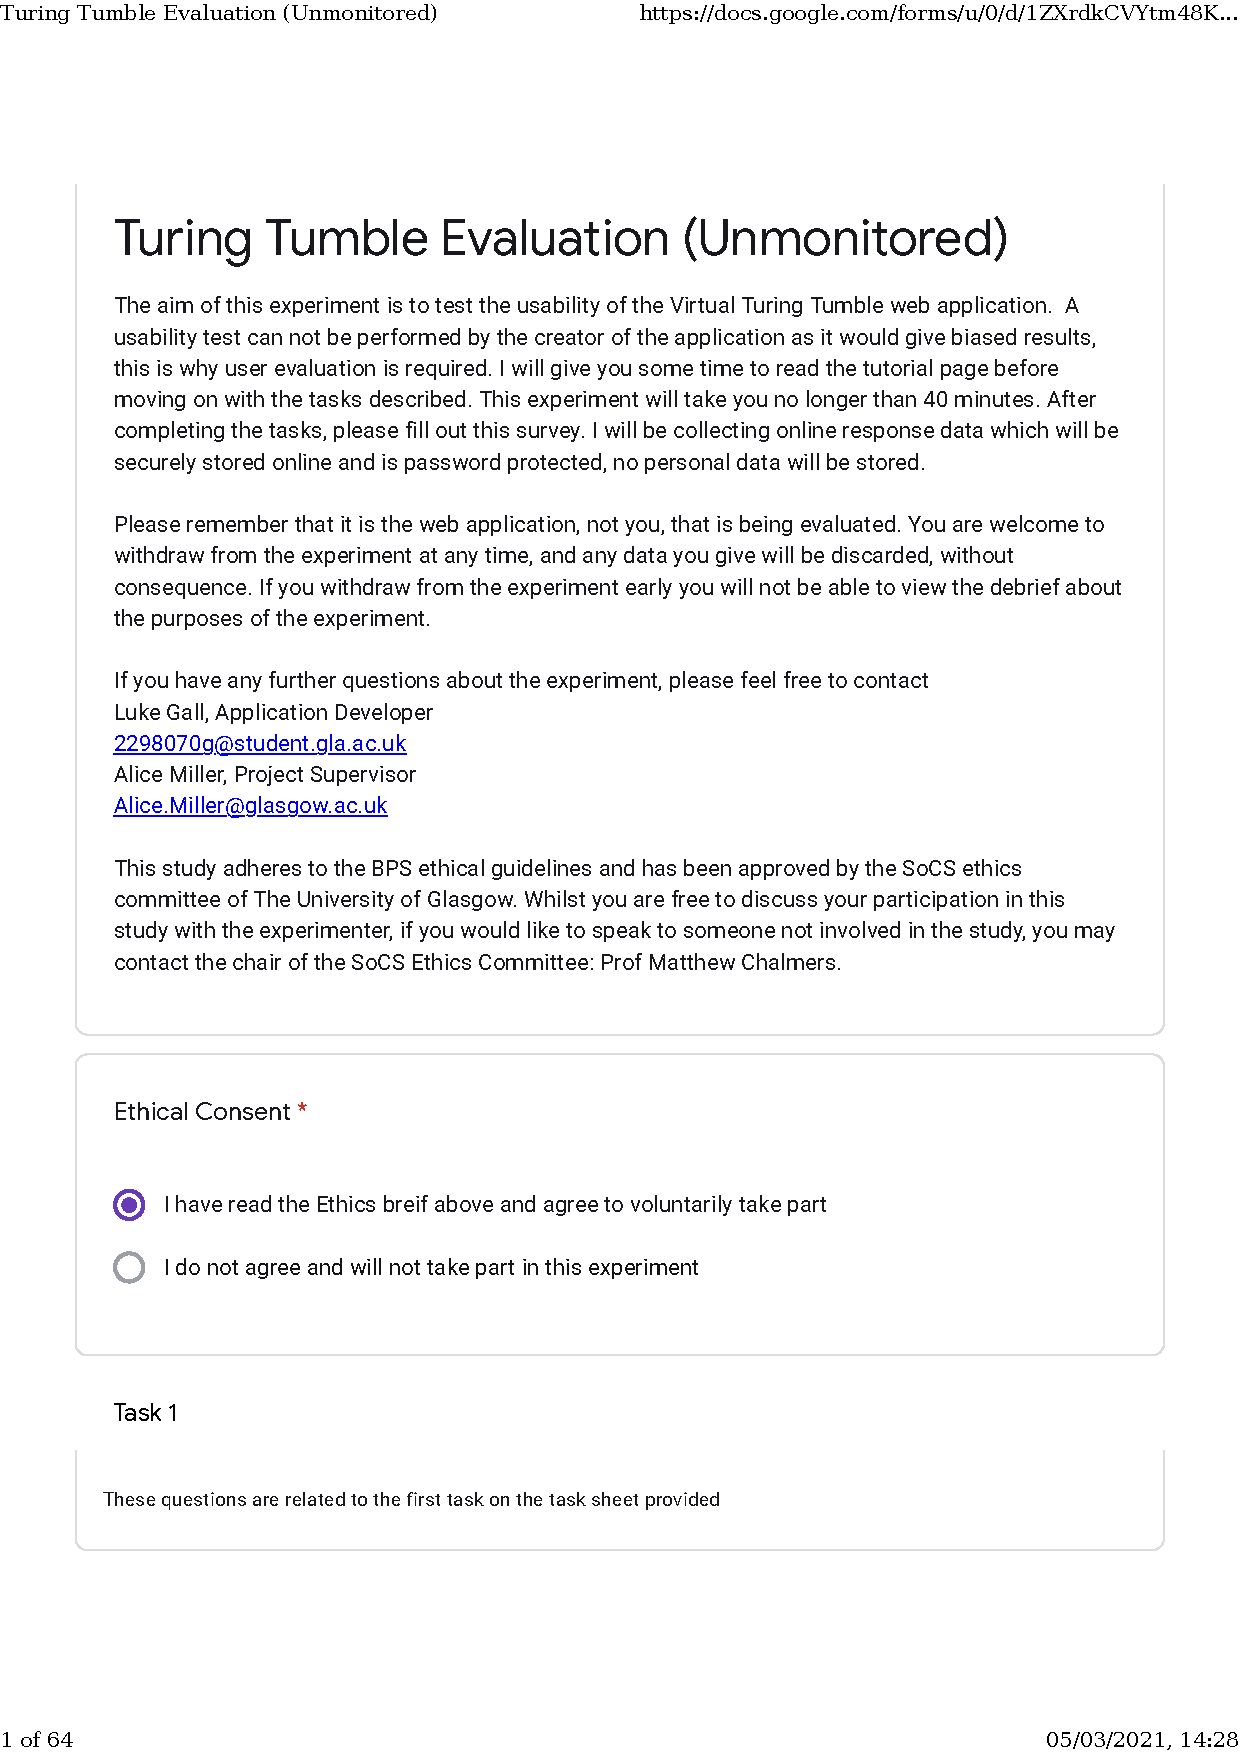
\includepdf[pages=-]{images/unmonitoredResponses1.pdf}
% 
\includepdf[pages=-]{images/unmonitoredResponses2.pdf}

% \section{Monitored Consent Form}
% This was form was sent out to possible users. Once signed and returned they were sent the task sheet.

% 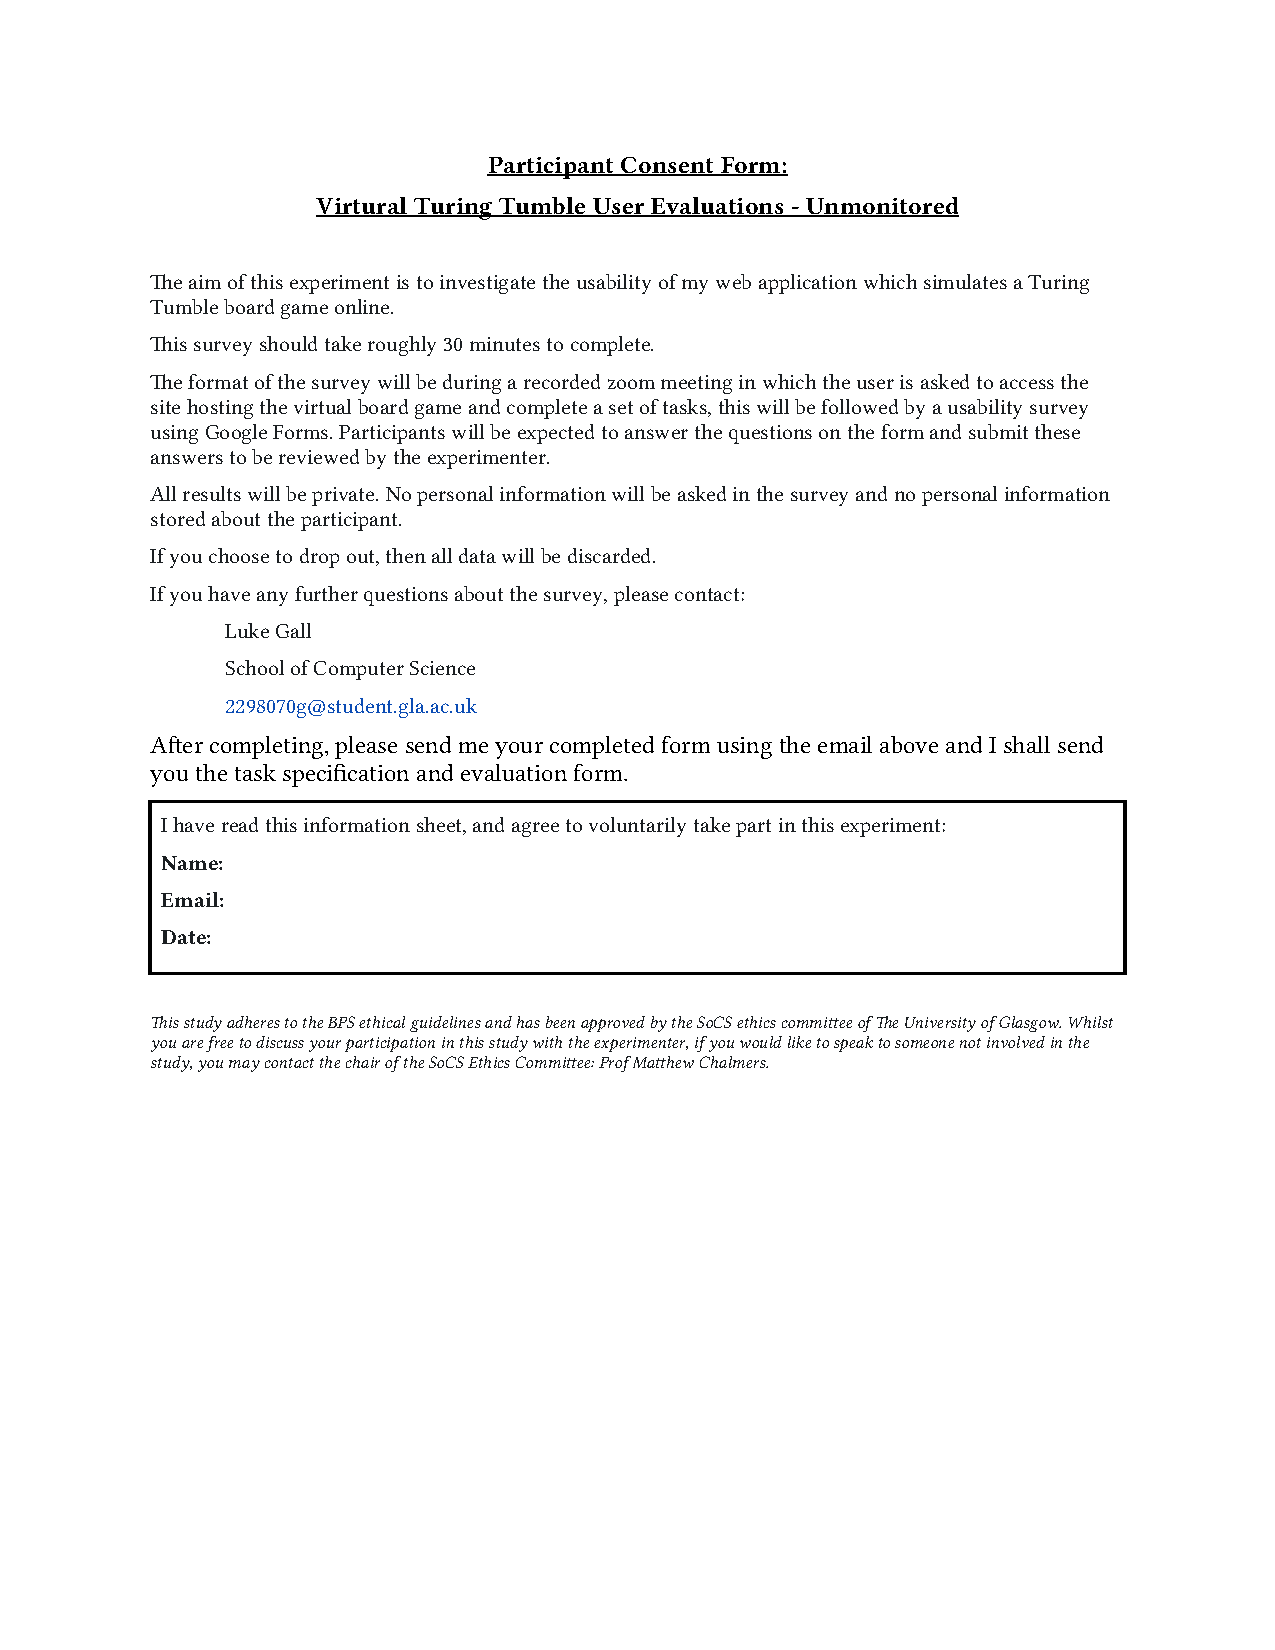
\includepdf{images/monitoredConsent.pdf}
\section{Monitored Task Sheet}
\label{section:monitored-tasks}

\includepdf[pages=-]{images/taskSpecMonitored.pdf}
\section{Monitored Evaluation Questions}
\label{section:mon-questions}
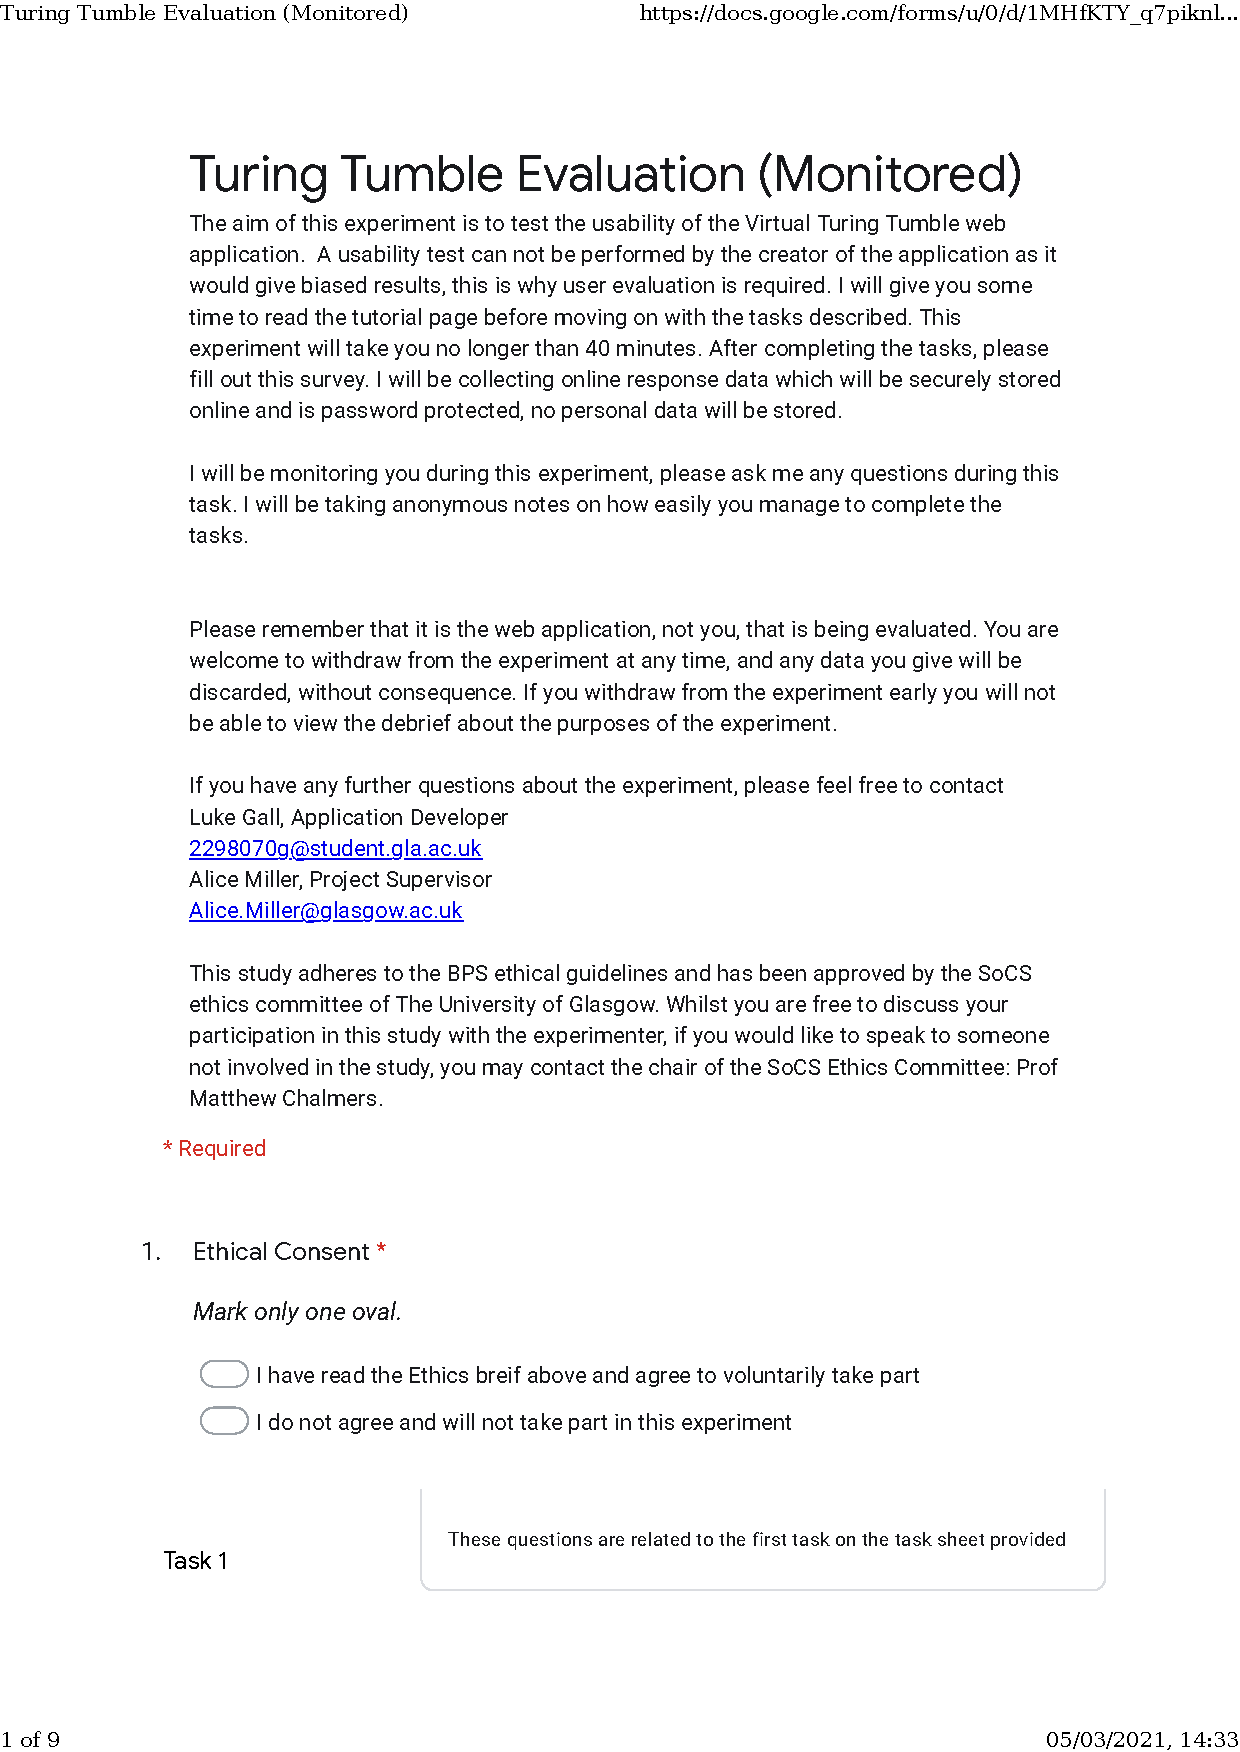
\includepdf[pages=-]{images/monitoredQuestions.pdf}
% \section{Monitored Evaluation Responses}
% 
\includepdf[pages=-]{images/monitoredResponses.pdf}
\section{Monitored Evaluation Notes}
\label{section:monitored-eval-notes}
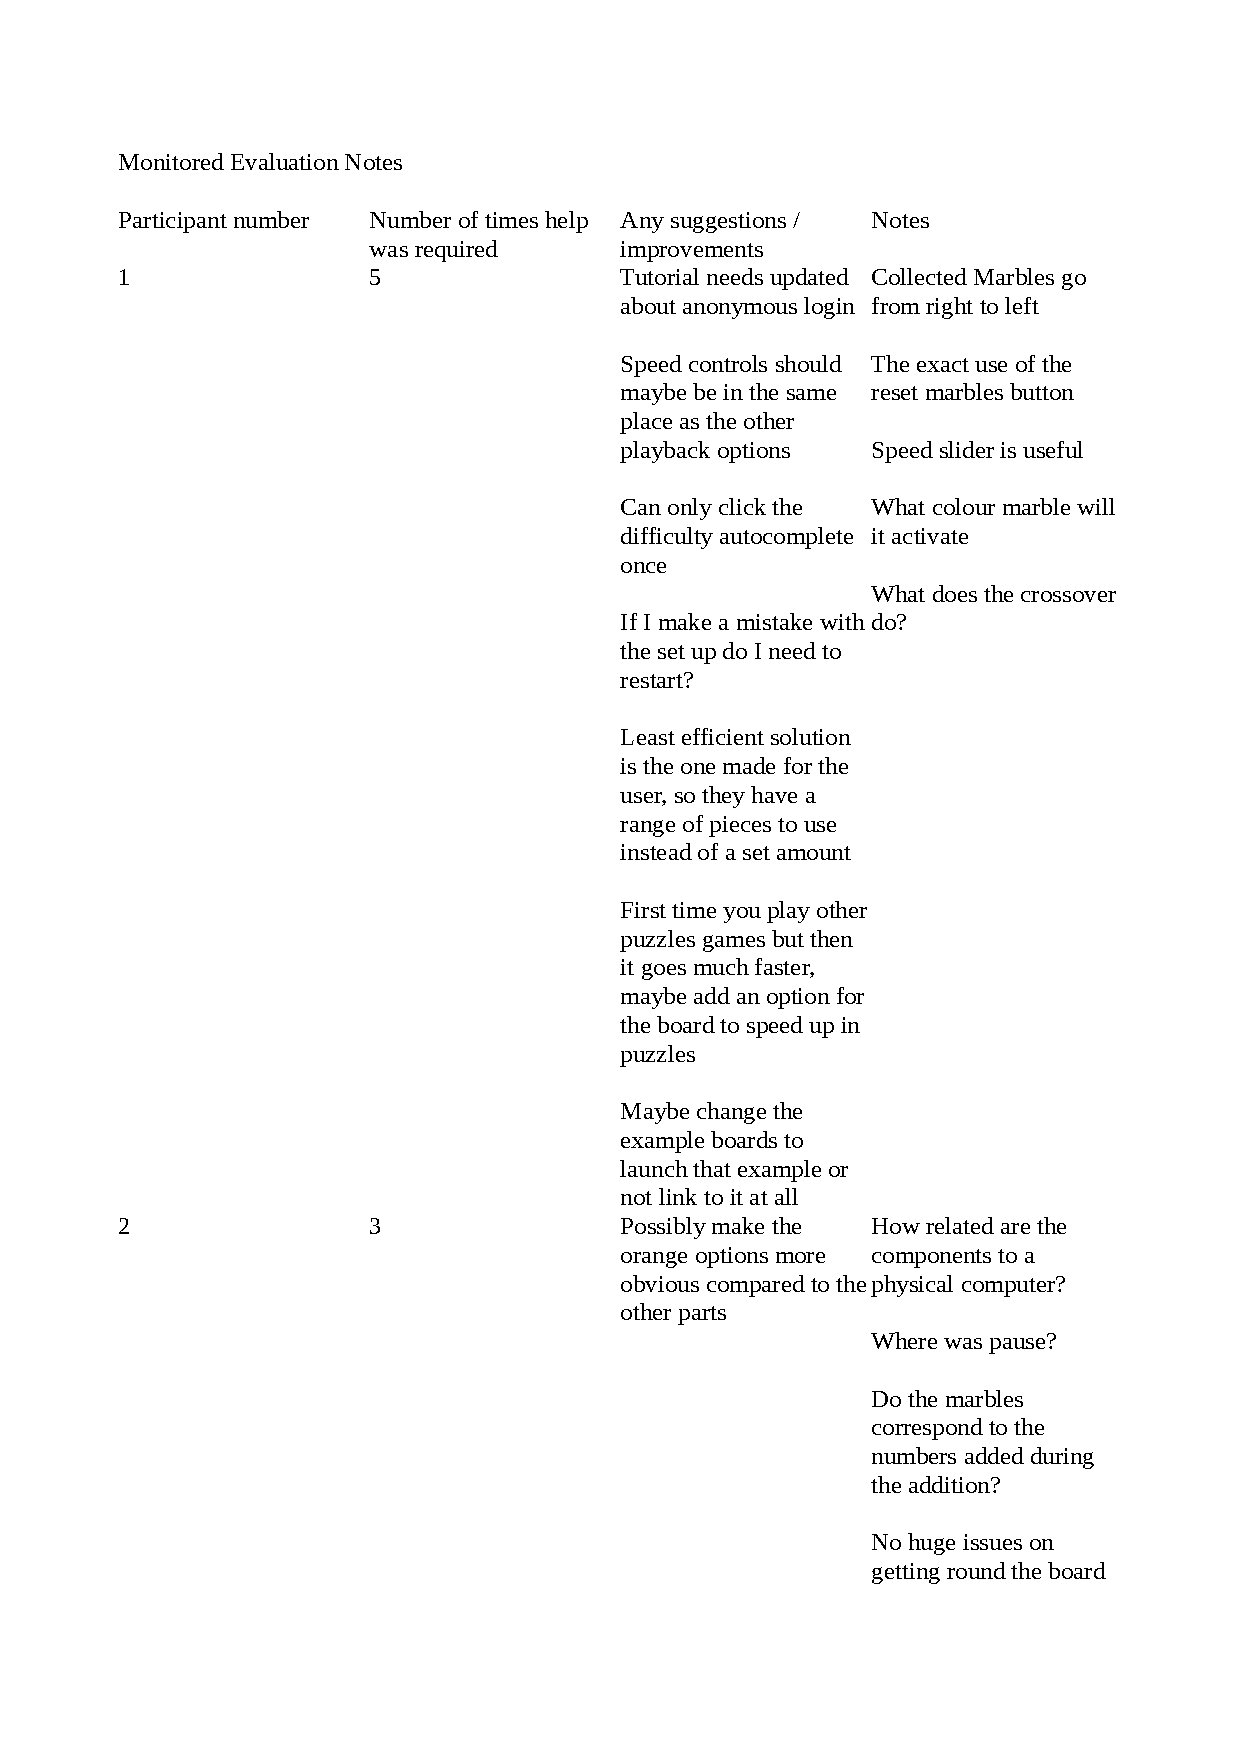
\includepdf[pages=-]{images/MonitoredEvalNotes.pdf}

\end{appendices}

%==================================================================================================================================
%   BIBLIOGRAPHY   

% The bibliography style is abbrvnat
% The bibliography always appears last, after the appendices.

\bibliographystyle{abbrvnat}

\bibliography{l4proj}

\end{document}
